% Options for packages loaded elsewhere
% Options for packages loaded elsewhere
\PassOptionsToPackage{unicode}{hyperref}
\PassOptionsToPackage{hyphens}{url}
\PassOptionsToPackage{dvipsnames,svgnames,x11names}{xcolor}
%
\documentclass[
  polish,
  letterpaper,
  DIV=11,
  numbers=noendperiod]{scrartcl}
\usepackage{xcolor}
\usepackage{amsmath,amssymb}
\setcounter{secnumdepth}{5}
\usepackage{iftex}
\ifPDFTeX
  \usepackage[T1]{fontenc}
  \usepackage[utf8]{inputenc}
  \usepackage{textcomp} % provide euro and other symbols
\else % if luatex or xetex
  \usepackage{unicode-math} % this also loads fontspec
  \defaultfontfeatures{Scale=MatchLowercase}
  \defaultfontfeatures[\rmfamily]{Ligatures=TeX,Scale=1}
\fi
\usepackage{lmodern}
\ifPDFTeX\else
  % xetex/luatex font selection
  \setmainfont[]{Times New Roman}
  \setsansfont[]{Times New Roman}
\fi
% Use upquote if available, for straight quotes in verbatim environments
\IfFileExists{upquote.sty}{\usepackage{upquote}}{}
\IfFileExists{microtype.sty}{% use microtype if available
  \usepackage[]{microtype}
  \UseMicrotypeSet[protrusion]{basicmath} % disable protrusion for tt fonts
}{}
\makeatletter
\@ifundefined{KOMAClassName}{% if non-KOMA class
  \IfFileExists{parskip.sty}{%
    \usepackage{parskip}
  }{% else
    \setlength{\parindent}{0pt}
    \setlength{\parskip}{6pt plus 2pt minus 1pt}}
}{% if KOMA class
  \KOMAoptions{parskip=half}}
\makeatother
% Make \paragraph and \subparagraph free-standing
\makeatletter
\ifx\paragraph\undefined\else
  \let\oldparagraph\paragraph
  \renewcommand{\paragraph}{
    \@ifstar
      \xxxParagraphStar
      \xxxParagraphNoStar
  }
  \newcommand{\xxxParagraphStar}[1]{\oldparagraph*{#1}\mbox{}}
  \newcommand{\xxxParagraphNoStar}[1]{\oldparagraph{#1}\mbox{}}
\fi
\ifx\subparagraph\undefined\else
  \let\oldsubparagraph\subparagraph
  \renewcommand{\subparagraph}{
    \@ifstar
      \xxxSubParagraphStar
      \xxxSubParagraphNoStar
  }
  \newcommand{\xxxSubParagraphStar}[1]{\oldsubparagraph*{#1}\mbox{}}
  \newcommand{\xxxSubParagraphNoStar}[1]{\oldsubparagraph{#1}\mbox{}}
\fi
\makeatother

\usepackage{color}
\usepackage{fancyvrb}
\newcommand{\VerbBar}{|}
\newcommand{\VERB}{\Verb[commandchars=\\\{\}]}
\DefineVerbatimEnvironment{Highlighting}{Verbatim}{commandchars=\\\{\}}
% Add ',fontsize=\small' for more characters per line
\usepackage{framed}
\definecolor{shadecolor}{RGB}{241,243,245}
\newenvironment{Shaded}{\begin{snugshade}}{\end{snugshade}}
\newcommand{\AlertTok}[1]{\textcolor[rgb]{0.68,0.00,0.00}{#1}}
\newcommand{\AnnotationTok}[1]{\textcolor[rgb]{0.37,0.37,0.37}{#1}}
\newcommand{\AttributeTok}[1]{\textcolor[rgb]{0.40,0.45,0.13}{#1}}
\newcommand{\BaseNTok}[1]{\textcolor[rgb]{0.68,0.00,0.00}{#1}}
\newcommand{\BuiltInTok}[1]{\textcolor[rgb]{0.00,0.23,0.31}{#1}}
\newcommand{\CharTok}[1]{\textcolor[rgb]{0.13,0.47,0.30}{#1}}
\newcommand{\CommentTok}[1]{\textcolor[rgb]{0.37,0.37,0.37}{#1}}
\newcommand{\CommentVarTok}[1]{\textcolor[rgb]{0.37,0.37,0.37}{\textit{#1}}}
\newcommand{\ConstantTok}[1]{\textcolor[rgb]{0.56,0.35,0.01}{#1}}
\newcommand{\ControlFlowTok}[1]{\textcolor[rgb]{0.00,0.23,0.31}{\textbf{#1}}}
\newcommand{\DataTypeTok}[1]{\textcolor[rgb]{0.68,0.00,0.00}{#1}}
\newcommand{\DecValTok}[1]{\textcolor[rgb]{0.68,0.00,0.00}{#1}}
\newcommand{\DocumentationTok}[1]{\textcolor[rgb]{0.37,0.37,0.37}{\textit{#1}}}
\newcommand{\ErrorTok}[1]{\textcolor[rgb]{0.68,0.00,0.00}{#1}}
\newcommand{\ExtensionTok}[1]{\textcolor[rgb]{0.00,0.23,0.31}{#1}}
\newcommand{\FloatTok}[1]{\textcolor[rgb]{0.68,0.00,0.00}{#1}}
\newcommand{\FunctionTok}[1]{\textcolor[rgb]{0.28,0.35,0.67}{#1}}
\newcommand{\ImportTok}[1]{\textcolor[rgb]{0.00,0.46,0.62}{#1}}
\newcommand{\InformationTok}[1]{\textcolor[rgb]{0.37,0.37,0.37}{#1}}
\newcommand{\KeywordTok}[1]{\textcolor[rgb]{0.00,0.23,0.31}{\textbf{#1}}}
\newcommand{\NormalTok}[1]{\textcolor[rgb]{0.00,0.23,0.31}{#1}}
\newcommand{\OperatorTok}[1]{\textcolor[rgb]{0.37,0.37,0.37}{#1}}
\newcommand{\OtherTok}[1]{\textcolor[rgb]{0.00,0.23,0.31}{#1}}
\newcommand{\PreprocessorTok}[1]{\textcolor[rgb]{0.68,0.00,0.00}{#1}}
\newcommand{\RegionMarkerTok}[1]{\textcolor[rgb]{0.00,0.23,0.31}{#1}}
\newcommand{\SpecialCharTok}[1]{\textcolor[rgb]{0.37,0.37,0.37}{#1}}
\newcommand{\SpecialStringTok}[1]{\textcolor[rgb]{0.13,0.47,0.30}{#1}}
\newcommand{\StringTok}[1]{\textcolor[rgb]{0.13,0.47,0.30}{#1}}
\newcommand{\VariableTok}[1]{\textcolor[rgb]{0.07,0.07,0.07}{#1}}
\newcommand{\VerbatimStringTok}[1]{\textcolor[rgb]{0.13,0.47,0.30}{#1}}
\newcommand{\WarningTok}[1]{\textcolor[rgb]{0.37,0.37,0.37}{\textit{#1}}}

\usepackage{longtable,booktabs,array}
\newcounter{none} % for unnumbered tables
\usepackage{calc} % for calculating minipage widths
% Correct order of tables after \paragraph or \subparagraph
\usepackage{etoolbox}
\makeatletter
\patchcmd\longtable{\par}{\if@noskipsec\mbox{}\fi\par}{}{}
\makeatother
% Allow footnotes in longtable head/foot
\IfFileExists{footnotehyper.sty}{\usepackage{footnotehyper}}{\usepackage{footnote}}
\makesavenoteenv{longtable}
\usepackage{graphicx}
\makeatletter
\newsavebox\pandoc@box
\newcommand*\pandocbounded[1]{% scales image to fit in text height/width
  \sbox\pandoc@box{#1}%
  \Gscale@div\@tempa{\textheight}{\dimexpr\ht\pandoc@box+\dp\pandoc@box\relax}%
  \Gscale@div\@tempb{\linewidth}{\wd\pandoc@box}%
  \ifdim\@tempb\p@<\@tempa\p@\let\@tempa\@tempb\fi% select the smaller of both
  \ifdim\@tempa\p@<\p@\scalebox{\@tempa}{\usebox\pandoc@box}%
  \else\usebox{\pandoc@box}%
  \fi%
}
% Set default figure placement to htbp
\def\fps@figure{htbp}
\makeatother


% definitions for citeproc citations
\NewDocumentCommand\citeproctext{}{}
\NewDocumentCommand\citeproc{mm}{%
  \begingroup\def\citeproctext{#2}\cite{#1}\endgroup}
\makeatletter
 % allow citations to break across lines
 \let\@cite@ofmt\@firstofone
 % avoid brackets around text for \cite:
 \def\@biblabel#1{}
 \def\@cite#1#2{{#1\if@tempswa , #2\fi}}
\makeatother
\newlength{\cslhangindent}
\setlength{\cslhangindent}{1.5em}
\newlength{\csllabelwidth}
\setlength{\csllabelwidth}{3em}
\newenvironment{CSLReferences}[2] % #1 hanging-indent, #2 entry-spacing
 {\begin{list}{}{%
  \setlength{\itemindent}{0pt}
  \setlength{\leftmargin}{0pt}
  \setlength{\parsep}{0pt}
  % turn on hanging indent if param 1 is 1
  \ifodd #1
   \setlength{\leftmargin}{\cslhangindent}
   \setlength{\itemindent}{-1\cslhangindent}
  \fi
  % set entry spacing
  \setlength{\itemsep}{#2\baselineskip}}}
 {\end{list}}
\usepackage{calc}
\newcommand{\CSLBlock}[1]{\hfill\break\parbox[t]{\linewidth}{\strut\ignorespaces#1\strut}}
\newcommand{\CSLLeftMargin}[1]{\parbox[t]{\csllabelwidth}{\strut#1\strut}}
\newcommand{\CSLRightInline}[1]{\parbox[t]{\linewidth - \csllabelwidth}{\strut#1\strut}}
\newcommand{\CSLIndent}[1]{\hspace{\cslhangindent}#1}

\ifLuaTeX
\usepackage[bidi=basic,shorthands=off]{babel}
\else
\usepackage[bidi=default,shorthands=off]{babel}
\fi
\ifPDFTeX
\else
\babelfont{rm}[]{Times New Roman}
\fi
\ifLuaTeX
  \usepackage{selnolig} % disable illegal ligatures
\fi


\setlength{\emergencystretch}{3em} % prevent overfull lines

\providecommand{\tightlist}{%
  \setlength{\itemsep}{0pt}\setlength{\parskip}{0pt}}



 


\KOMAoption{captions}{tableheading}
\addtokomafont{disposition}{\rmfamily}
\addtokomafont{caption}{\rmfamily}
\addtokomafont{captionlabel}{\rmfamily}
\usepackage{etoolbox}
\usepackage{fancyhdr}
\pretocmd{\section}{\clearpage}{}{}
\let\oldlistoffigures\listoffigures
\renewcommand{\listoffigures}{{\rmfamily\oldlistoffigures}}
\KOMAoptions{listof=totoc}
\usepackage{hyperref}
\hypersetup{linkcolor=black, urlcolor=black, citecolor=black}
\pagestyle{fancy}
\fancyhf{}
\fancyfoot[R]{\thepage}
\renewcommand{\headrulewidth}{0pt}
\fancypagestyle{plain}{\fancyhf{}\fancyfoot[R]{\thepage}\renewcommand{\headrulewidth}{0pt}}
\AtBeginDocument{\thispagestyle{empty}\setcounter{page}{0}}
\fancypagestyle{empty}{\fancyhf{}\renewcommand{\headrulewidth}{0pt}}
\fancypagestyle{plain}{\fancyhf{}\renewcommand{\headrulewidth}{0pt}}
\makeatletter
\@ifpackageloaded{caption}{}{\usepackage{caption}}
\AtBeginDocument{%
\ifdefined\contentsname
  \renewcommand*\contentsname{Spis treści}
\else
  \newcommand\contentsname{Spis treści}
\fi
\ifdefined\listfigurename
  \renewcommand*\listfigurename{Spis rycin}
\else
  \newcommand\listfigurename{Spis rycin}
\fi
\ifdefined\listtablename
  \renewcommand*\listtablename{Spis tabel}
\else
  \newcommand\listtablename{Spis tabel}
\fi
\ifdefined\figurename
  \renewcommand*\figurename{Rysunek}
\else
  \newcommand\figurename{Rysunek}
\fi
\ifdefined\tablename
  \renewcommand*\tablename{Tabela}
\else
  \newcommand\tablename{Tabela}
\fi
}
\@ifpackageloaded{float}{}{\usepackage{float}}
\floatstyle{ruled}
\@ifundefined{c@chapter}{\newfloat{codelisting}{h}{lop}}{\newfloat{codelisting}{h}{lop}[chapter]}
\floatname{codelisting}{Wykaz}
\newcommand*\listoflistings{\listof{codelisting}{Spis wykazów}}
\makeatother
\makeatletter
\makeatother
\makeatletter
\@ifpackageloaded{caption}{}{\usepackage{caption}}
\@ifpackageloaded{subcaption}{}{\usepackage{subcaption}}
\makeatother
\usepackage{bookmark}
\IfFileExists{xurl.sty}{\usepackage{xurl}}{} % add URL line breaks if available
\urlstyle{same}
\hypersetup{
  pdftitle={Predykcja cen akcji spółki PZU oraz korelacja z czynnikimi gospodarczymi},
  pdfauthor={Maciej Kuchcik; Andrzej Szuwald},
  pdflang={pl},
  colorlinks=true,
  linkcolor={blue},
  filecolor={Maroon},
  citecolor={Blue},
  urlcolor={Blue},
  pdfcreator={LaTeX via pandoc}}


\title{Predykcja cen akcji spółki PZU oraz korelacja z czynnikimi
gospodarczymi}
\usepackage{etoolbox}
\makeatletter
\providecommand{\subtitle}[1]{% add subtitle to \maketitle
  \apptocmd{\@title}{\par {\large #1 \par}}{}{}
}
\makeatother
\subtitle{Analiza i prognozowanie wielowymiarowego szeregu czasowego}
\author{Maciej Kuchcik \and Andrzej Szuwald}
\date{2026-06-18}
\begin{document}
\maketitle

\renewcommand*\contentsname{Spis treści}
{
\setcounter{tocdepth}{3}
\tableofcontents
}

\section*{Inicjalizacja}\label{inicjalizacja}
\addcontentsline{toc}{section}{Inicjalizacja}

W tej części ładowane są biblioteki oraz inicjalizowane są zmienne.

Zmienna \(FORMAT\) jest flagą, która wskazuje jaki silnik został
wykorzystany podczas renderowania. Wykorzystane jest to podczas
tworzenia wykresów. Język R wtedy decyduje, czy wyrenderować wersję
internetową (HTML: grafy interaktywne, zmieniające kolor w zależności od
motywu), lub dokumentową (PDF: stałe zdjęcia).

\begin{Shaded}
\begin{Highlighting}[]
\ControlFlowTok{if}\NormalTok{ (}\SpecialCharTok{!}\FunctionTok{require}\NormalTok{(}\StringTok{"quantmod"}\NormalTok{)) }\FunctionTok{install.packages}\NormalTok{(}\StringTok{"quantmod"}\NormalTok{)}
\FunctionTok{library}\NormalTok{(quantmod)}
\FunctionTok{library}\NormalTok{(ggplot2)}
\ControlFlowTok{if}\NormalTok{ (}\SpecialCharTok{!}\FunctionTok{require}\NormalTok{(}\StringTok{"readxl"}\NormalTok{)) }\FunctionTok{install.packages}\NormalTok{(}\StringTok{"readxl"}\NormalTok{)}
\FunctionTok{library}\NormalTok{(readxl)}
\ControlFlowTok{if}\NormalTok{ (}\SpecialCharTok{!}\FunctionTok{require}\NormalTok{(}\StringTok{"tseries"}\NormalTok{)) }\FunctionTok{install.packages}\NormalTok{(}\StringTok{"tseries"}\NormalTok{)}
\FunctionTok{library}\NormalTok{(tseries)}
\ControlFlowTok{if}\NormalTok{ (}\SpecialCharTok{!}\FunctionTok{require}\NormalTok{(}\StringTok{"highcharter"}\NormalTok{)) }\FunctionTok{install.packages}\NormalTok{(}\StringTok{"highcharter"}\NormalTok{)}
\FunctionTok{library}\NormalTok{(}\StringTok{"highcharter"}\NormalTok{)}
\ControlFlowTok{if}\NormalTok{ (}\SpecialCharTok{!}\FunctionTok{require}\NormalTok{(}\StringTok{"forecast"}\NormalTok{)) }\FunctionTok{install.packages}\NormalTok{(}\StringTok{"forecast"}\NormalTok{)}
\FunctionTok{library}\NormalTok{(forecast)}
\CommentTok{\#if (!require("midasr")) install.packages("midasr")}
\CommentTok{\#library(midasr)}
\ControlFlowTok{if}\NormalTok{ (}\SpecialCharTok{!}\FunctionTok{require}\NormalTok{(}\StringTok{"vars"}\NormalTok{)) }\FunctionTok{install.packages}\NormalTok{(}\StringTok{"vars"}\NormalTok{)}
\FunctionTok{library}\NormalTok{(vars)}

\FunctionTok{options}\NormalTok{(}\AttributeTok{highcharter.lang =} \FunctionTok{list}\NormalTok{(}
    \AttributeTok{months =} \FunctionTok{c}\NormalTok{(}\StringTok{"Styczeń"}\NormalTok{, }\StringTok{"Luty"}\NormalTok{, }\StringTok{"Marzec"}\NormalTok{, }\StringTok{"Kwiecień"}\NormalTok{, }\StringTok{"Maj"}\NormalTok{, }\StringTok{"Czerwiec"}\NormalTok{, }
               \StringTok{"Lipiec"}\NormalTok{, }\StringTok{"Sierpień"}\NormalTok{, }\StringTok{"Wrzesień"}\NormalTok{, }\StringTok{"Październik"}\NormalTok{, }
               \StringTok{"Listopad"}\NormalTok{, }\StringTok{"Grudzień"}\NormalTok{),}
    \AttributeTok{shortMonths =} \FunctionTok{c}\NormalTok{(}\StringTok{"Sty"}\NormalTok{, }\StringTok{"Lut"}\NormalTok{, }\StringTok{"Mar"}\NormalTok{, }\StringTok{"Kwi"}\NormalTok{, }\StringTok{"Maj"}\NormalTok{, }\StringTok{"Cze"}\NormalTok{, }
                    \StringTok{"Lip"}\NormalTok{, }\StringTok{"Sie"}\NormalTok{, }\StringTok{"Wrz"}\NormalTok{, }\StringTok{"Paź"}\NormalTok{, }\StringTok{"Lis"}\NormalTok{, }\StringTok{"Gru"}\NormalTok{),}
    \AttributeTok{weekdays =} \FunctionTok{c}\NormalTok{(}\StringTok{"Niedziela"}\NormalTok{, }\StringTok{"Poniedziałek"}\NormalTok{, }\StringTok{"Wtorek"}\NormalTok{, }\StringTok{"Środa"}\NormalTok{, }\StringTok{"Czwartek"}\NormalTok{, }
                 \StringTok{"Piątek"}\NormalTok{, }\StringTok{"Sobota"}\NormalTok{),}
    \AttributeTok{shortWeekdays =} \FunctionTok{c}\NormalTok{(}\StringTok{"Nie"}\NormalTok{, }\StringTok{"Pon"}\NormalTok{, }\StringTok{"Wto"}\NormalTok{, }\StringTok{"Śro"}\NormalTok{, }\StringTok{"Czw"}\NormalTok{, }\StringTok{"Pią"}\NormalTok{, }\StringTok{"Sob"}\NormalTok{),}
    \AttributeTok{rangeSelectorFrom =} \StringTok{"Od"}\NormalTok{,}
    \AttributeTok{rangeSelectorTo =} \StringTok{"Do"}\NormalTok{,}
    \AttributeTok{rangeSelectorZoom =} \StringTok{"Zakres"}\NormalTok{,}
    \AttributeTok{loading =} \StringTok{"Ładowanie..."}
\NormalTok{  )}
\NormalTok{)}

\NormalTok{FORMAT}\OtherTok{\textless{}{-}}\NormalTok{knitr}\SpecialCharTok{::}\FunctionTok{pandoc\_to}\NormalTok{()}
\ControlFlowTok{if}\NormalTok{ (}\FunctionTok{is.null}\NormalTok{(FORMAT)) \{}
\NormalTok{  FORMAT }\OtherTok{\textless{}{-}} \StringTok{"html"}
\NormalTok{\}}
\end{Highlighting}
\end{Shaded}

\begin{Shaded}
\begin{Highlighting}[]
\CommentTok{\# Autor: Maciej Kuchcik}

\NormalTok{rysuj\_rdzen }\OtherTok{\textless{}{-}} \ControlFlowTok{function}\NormalTok{(dane\_ts, tytul, etykieta\_y, kolory) \{}
  \FunctionTok{plot}\NormalTok{(dane\_ts, }\AttributeTok{xlab =} \StringTok{"Rok"}\NormalTok{, }\AttributeTok{ylab =}\NormalTok{ etykieta\_y, }
       \AttributeTok{main =}\NormalTok{ tytul, }\AttributeTok{col =}\NormalTok{ kolory}\SpecialCharTok{$}\NormalTok{linia, }\AttributeTok{lwd =} \DecValTok{2}\NormalTok{)}
  \FunctionTok{grid}\NormalTok{(}\AttributeTok{col =}\NormalTok{ kolory}\SpecialCharTok{$}\NormalTok{siatka)}
  
\NormalTok{  start\_zagrozenia }\OtherTok{\textless{}{-}} \DecValTok{2020} \SpecialCharTok{+}\NormalTok{ (}\DecValTok{3} \SpecialCharTok{{-}} \DecValTok{1}\NormalTok{) }\SpecialCharTok{/} \DecValTok{12}
\NormalTok{  koniec\_zagrozenia }\OtherTok{\textless{}{-}} \DecValTok{2023} \SpecialCharTok{+}\NormalTok{ (}\DecValTok{6} \SpecialCharTok{{-}} \DecValTok{1}\NormalTok{) }\SpecialCharTok{/} \DecValTok{12}
  
  \FunctionTok{rect}\NormalTok{(start\_zagrozenia, }\FunctionTok{par}\NormalTok{(}\StringTok{"usr"}\NormalTok{)[}\DecValTok{3}\NormalTok{], koniec\_zagrozenia, }\FunctionTok{par}\NormalTok{(}\StringTok{"usr"}\NormalTok{)[}\DecValTok{4}\NormalTok{], }
       \AttributeTok{col =} \FunctionTok{rgb}\NormalTok{(}\DecValTok{1}\NormalTok{, }\DecValTok{0}\NormalTok{, }\DecValTok{0}\NormalTok{, }\FloatTok{0.12}\NormalTok{), }\AttributeTok{border =} \ConstantTok{NA}\NormalTok{)}
  
  \FunctionTok{legend}\NormalTok{(}\StringTok{"topleft"}\NormalTok{, }\AttributeTok{legend =} \StringTok{"COVID"}\NormalTok{, }\AttributeTok{fill =} \FunctionTok{rgb}\NormalTok{(}\DecValTok{1}\NormalTok{, }\DecValTok{0}\NormalTok{, }\DecValTok{0}\NormalTok{, }\FloatTok{0.12}\NormalTok{), }
         \AttributeTok{border =} \ConstantTok{NA}\NormalTok{, }\AttributeTok{bty =} \StringTok{"n"}\NormalTok{)}
\NormalTok{\}}

\NormalTok{rysuj\_makro\_wykres }\OtherTok{\textless{}{-}} \ControlFlowTok{function}\NormalTok{(dane\_ts, tytul, etykieta\_y, }\AttributeTok{format =} \StringTok{"pdf"}\NormalTok{) \{}
  \CommentTok{\# Zawsze: jasna}
\NormalTok{  jasne\_kolory }\OtherTok{\textless{}{-}} \FunctionTok{list}\NormalTok{(}\AttributeTok{linia =} \StringTok{"royalblue"}\NormalTok{, }\AttributeTok{siatka =} \StringTok{"\#cccccc"}\NormalTok{)}
  \FunctionTok{par}\NormalTok{(}\AttributeTok{bg =} \StringTok{"white"}\NormalTok{, }\AttributeTok{col.axis =} \StringTok{"black"}\NormalTok{, }\AttributeTok{col.lab =} \StringTok{"black"}\NormalTok{, }
      \AttributeTok{col.main =} \StringTok{"black"}\NormalTok{, }\AttributeTok{fg =} \StringTok{"black"}\NormalTok{)}
  \FunctionTok{rysuj\_rdzen}\NormalTok{(dane\_ts, }\FunctionTok{ifelse}\NormalTok{(format }\SpecialCharTok{==} \StringTok{"html"}\NormalTok{, tytul, }\StringTok{""}\NormalTok{),}
              
\NormalTok{              etykieta\_y, jasne\_kolory)}
  
  \CommentTok{\# HTML: rysujemy też wersję ciemną}
  \ControlFlowTok{if}\NormalTok{ (format }\SpecialCharTok{==} \StringTok{"html"}\NormalTok{) \{}
    \FunctionTok{par}\NormalTok{(}\AttributeTok{bg =} \StringTok{"\#222222"}\NormalTok{, }\AttributeTok{col.axis =} \StringTok{"\#dddddd"}\NormalTok{, }\AttributeTok{col.lab =} \StringTok{"\#dddddd"}\NormalTok{, }
        \AttributeTok{col.main =} \StringTok{"\#dddddd"}\NormalTok{, }\AttributeTok{fg =} \StringTok{"\#dddddd"}\NormalTok{)}
\NormalTok{    ciemne\_kolory }\OtherTok{\textless{}{-}} \FunctionTok{list}\NormalTok{(}\AttributeTok{linia =} \StringTok{"\#6baed6"}\NormalTok{, }\AttributeTok{siatka =} \StringTok{"\#444444"}\NormalTok{)}
    \FunctionTok{rysuj\_rdzen}\NormalTok{(dane\_ts, tytul, etykieta\_y, ciemne\_kolory)}
    
    \CommentTok{\# Reset po HTML}
    \FunctionTok{par}\NormalTok{(}\AttributeTok{bg =} \StringTok{"white"}\NormalTok{, }\AttributeTok{col.axis =} \StringTok{"black"}\NormalTok{, }\AttributeTok{col.lab =} \StringTok{"black"}\NormalTok{, }
        \AttributeTok{col.main =} \StringTok{"black"}\NormalTok{, }\AttributeTok{fg =} \StringTok{"black"}\NormalTok{)}
\NormalTok{  \}}
\NormalTok{\}}
\end{Highlighting}
\end{Shaded}

\begin{Shaded}
\begin{Highlighting}[]
\CommentTok{\# Autor: Maciej Kuchcik}

\NormalTok{wykres\_predykcji }\OtherTok{\textless{}{-}} \ControlFlowTok{function}\NormalTok{(daty, cena\_real, cena\_pred, blad,}
\NormalTok{                              tytul, nazwa\_modelu, }\AttributeTok{format =}\NormalTok{ FORMAT) \{}
  \ControlFlowTok{if}\NormalTok{ (format }\SpecialCharTok{==} \StringTok{"html"}\NormalTok{) \{}
\NormalTok{    df }\OtherTok{\textless{}{-}} \FunctionTok{data.frame}\NormalTok{(}
      \AttributeTok{x           =} \FunctionTok{as.numeric}\NormalTok{(}\FunctionTok{as.POSIXct}\NormalTok{(daty)) }\SpecialCharTok{*} \DecValTok{1000}\NormalTok{,}
      \AttributeTok{rzeczywiste =}\NormalTok{ cena\_real,}
      \AttributeTok{prognoza    =}\NormalTok{ cena\_pred,}
      \AttributeTok{blad        =}\NormalTok{ blad}
\NormalTok{    )}
    \FunctionTok{highchart}\NormalTok{() }\SpecialCharTok{|\textgreater{}}
      \FunctionTok{hc\_title}\NormalTok{(}\AttributeTok{text =}\NormalTok{ tytul) }\SpecialCharTok{|\textgreater{}}
      \FunctionTok{hc\_xAxis}\NormalTok{(}\AttributeTok{type =} \StringTok{"datetime"}\NormalTok{) }\SpecialCharTok{|\textgreater{}}
      \FunctionTok{hc\_yAxis\_multiples}\NormalTok{(}
        \FunctionTok{list}\NormalTok{(}\AttributeTok{title =} \FunctionTok{list}\NormalTok{(}\AttributeTok{text =} \StringTok{"Cena zamknięcia (zł)"}\NormalTok{), }\AttributeTok{opposite =} \ConstantTok{FALSE}\NormalTok{),}
        \FunctionTok{list}\NormalTok{(}\AttributeTok{title =} \FunctionTok{list}\NormalTok{(}\AttributeTok{text =} \StringTok{"Błąd (zł)"}\NormalTok{), }\AttributeTok{opposite =} \ConstantTok{TRUE}\NormalTok{, }\AttributeTok{gridLineWidth =} \DecValTok{0}\NormalTok{)}
\NormalTok{      ) }\SpecialCharTok{|\textgreater{}}
      \FunctionTok{hc\_add\_series}\NormalTok{(}
        \AttributeTok{data =} \FunctionTok{list\_parse2}\NormalTok{(}\FunctionTok{data.frame}\NormalTok{(}\AttributeTok{x =}\NormalTok{ df}\SpecialCharTok{$}\NormalTok{x, }\AttributeTok{y =}\NormalTok{ df}\SpecialCharTok{$}\NormalTok{rzeczywiste)),}
        \AttributeTok{type =} \StringTok{"line"}\NormalTok{, }\AttributeTok{name =} \StringTok{"Rzeczywista"}\NormalTok{, }\AttributeTok{color =} \StringTok{"\#2196F3"}\NormalTok{, }\AttributeTok{yAxis =} \DecValTok{0}
\NormalTok{      ) }\SpecialCharTok{|\textgreater{}}
      \FunctionTok{hc\_add\_series}\NormalTok{(}
        \AttributeTok{data =} \FunctionTok{list\_parse2}\NormalTok{(}\FunctionTok{data.frame}\NormalTok{(}\AttributeTok{x =}\NormalTok{ df}\SpecialCharTok{$}\NormalTok{x, }\AttributeTok{y =}\NormalTok{ df}\SpecialCharTok{$}\NormalTok{prognoza)),}
        \AttributeTok{type =} \StringTok{"line"}\NormalTok{, }\AttributeTok{name =} \FunctionTok{paste0}\NormalTok{(}\StringTok{"Prognoza "}\NormalTok{, nazwa\_modelu),}
        \AttributeTok{color =} \StringTok{"\#FF9800"}\NormalTok{, }\AttributeTok{dashStyle =} \StringTok{"ShortDash"}\NormalTok{, }\AttributeTok{yAxis =} \DecValTok{0}
\NormalTok{      ) }\SpecialCharTok{|\textgreater{}}
      \FunctionTok{hc\_add\_series}\NormalTok{(}
        \AttributeTok{data =} \FunctionTok{list\_parse2}\NormalTok{(}\FunctionTok{data.frame}\NormalTok{(}\AttributeTok{x =}\NormalTok{ df}\SpecialCharTok{$}\NormalTok{x, }\AttributeTok{y =}\NormalTok{ df}\SpecialCharTok{$}\NormalTok{blad)),}
        \AttributeTok{type =} \StringTok{"line"}\NormalTok{, }\AttributeTok{name =} \StringTok{"Błąd"}\NormalTok{, }\AttributeTok{color =} \StringTok{"rgba(229,57,53,0.5)"}\NormalTok{, }\AttributeTok{yAxis =} \DecValTok{1}
\NormalTok{      ) }\SpecialCharTok{|\textgreater{}}
      \FunctionTok{hc\_tooltip}\NormalTok{(}\AttributeTok{valueDecimals =} \DecValTok{2}\NormalTok{, }\AttributeTok{valueSuffix =} \StringTok{" zł"}\NormalTok{, }\AttributeTok{shared =} \ConstantTok{TRUE}\NormalTok{) }\SpecialCharTok{|\textgreater{}}
      \FunctionTok{hc\_legend}\NormalTok{(}\AttributeTok{enabled =} \ConstantTok{TRUE}\NormalTok{) }\SpecialCharTok{|\textgreater{}}
      \FunctionTok{hc\_rangeSelector}\NormalTok{(}\AttributeTok{enabled =} \ConstantTok{TRUE}\NormalTok{) }\SpecialCharTok{|\textgreater{}}
      \FunctionTok{hc\_scrollbar}\NormalTok{(}\AttributeTok{enabled =} \ConstantTok{TRUE}\NormalTok{)}
\NormalTok{  \} }\ControlFlowTok{else}\NormalTok{ \{}
    \FunctionTok{par}\NormalTok{(}\AttributeTok{bg =} \StringTok{"white"}\NormalTok{, }\AttributeTok{col.axis =} \StringTok{"black"}\NormalTok{, }\AttributeTok{col.lab =} \StringTok{"black"}\NormalTok{,}
        \AttributeTok{col.main =} \StringTok{"black"}\NormalTok{, }\AttributeTok{fg =} \StringTok{"black"}\NormalTok{)}
    \FunctionTok{plot}\NormalTok{(daty, cena\_real, }\AttributeTok{type =} \StringTok{"l"}\NormalTok{, }\AttributeTok{col =} \StringTok{"royalblue"}\NormalTok{, }\AttributeTok{lwd =} \FloatTok{1.5}\NormalTok{,}
         \AttributeTok{xlab =} \StringTok{"Data"}\NormalTok{, }\AttributeTok{ylab =} \StringTok{"Cena zamknięcia (zł)"}\NormalTok{, }\AttributeTok{main =}\NormalTok{ tytul)}
    \FunctionTok{lines}\NormalTok{(daty, cena\_pred, }\AttributeTok{col =} \StringTok{"tomato"}\NormalTok{, }\AttributeTok{lwd =} \FloatTok{1.5}\NormalTok{, }\AttributeTok{lty =} \DecValTok{2}\NormalTok{)}
    \FunctionTok{grid}\NormalTok{(}\AttributeTok{col =} \StringTok{"\#cccccc"}\NormalTok{)}
    \FunctionTok{par}\NormalTok{(}\AttributeTok{new =} \ConstantTok{TRUE}\NormalTok{)}
    \FunctionTok{plot}\NormalTok{(daty, blad, }\AttributeTok{type =} \StringTok{"l"}\NormalTok{, }\AttributeTok{col =} \FunctionTok{adjustcolor}\NormalTok{(}\StringTok{"red3"}\NormalTok{, }\AttributeTok{alpha.f =} \FloatTok{0.4}\NormalTok{),}
         \AttributeTok{lwd =} \DecValTok{1}\NormalTok{, }\AttributeTok{axes =} \ConstantTok{FALSE}\NormalTok{, }\AttributeTok{xlab =} \StringTok{""}\NormalTok{, }\AttributeTok{ylab =} \StringTok{""}\NormalTok{)}
    \FunctionTok{axis}\NormalTok{(}\DecValTok{4}\NormalTok{, }\AttributeTok{col =} \StringTok{"red3"}\NormalTok{, }\AttributeTok{col.axis =} \StringTok{"red3"}\NormalTok{)}
    \FunctionTok{mtext}\NormalTok{(}\StringTok{"Błąd (zł)"}\NormalTok{, }\AttributeTok{side =} \DecValTok{4}\NormalTok{, }\AttributeTok{line =} \DecValTok{3}\NormalTok{, }\AttributeTok{col =} \StringTok{"red3"}\NormalTok{)}
    \FunctionTok{legend}\NormalTok{(}\StringTok{"topleft"}\NormalTok{,}
           \AttributeTok{legend =} \FunctionTok{c}\NormalTok{(}\StringTok{"Rzeczywista"}\NormalTok{, }\FunctionTok{paste0}\NormalTok{(}\StringTok{"Prognoza "}\NormalTok{, nazwa\_modelu), }\StringTok{"Błąd"}\NormalTok{),}
           \AttributeTok{col =} \FunctionTok{c}\NormalTok{(}\StringTok{"royalblue"}\NormalTok{, }\StringTok{"tomato"}\NormalTok{, }\StringTok{"red3"}\NormalTok{),}
           \AttributeTok{lty =} \FunctionTok{c}\NormalTok{(}\DecValTok{1}\NormalTok{, }\DecValTok{2}\NormalTok{, }\DecValTok{1}\NormalTok{), }\AttributeTok{lwd =} \DecValTok{2}\NormalTok{, }\AttributeTok{bty =} \StringTok{"n"}\NormalTok{)}
\NormalTok{  \}}
\NormalTok{\}}
\end{Highlighting}
\end{Shaded}

\begin{Shaded}
\begin{Highlighting}[]
\CommentTok{\# Autor: Maciej Kuchcik}

\NormalTok{oblicz\_metryki }\OtherTok{\textless{}{-}} \ControlFlowTok{function}\NormalTok{(blad, cena\_real) \{}
  \FunctionTok{c}\NormalTok{(}
    \AttributeTok{MAE  =} \FunctionTok{mean}\NormalTok{(}\FunctionTok{abs}\NormalTok{(blad)),}
    \AttributeTok{RMSE =} \FunctionTok{sqrt}\NormalTok{(}\FunctionTok{mean}\NormalTok{(blad}\SpecialCharTok{\^{}}\DecValTok{2}\NormalTok{)),}
    \AttributeTok{MAPE =} \FunctionTok{mean}\NormalTok{(}\FunctionTok{abs}\NormalTok{(blad }\SpecialCharTok{/}\NormalTok{ cena\_real)) }\SpecialCharTok{*} \DecValTok{100}
\NormalTok{  )}
\NormalTok{\}}
\end{Highlighting}
\end{Shaded}

\begin{Shaded}
\begin{Highlighting}[]
\CommentTok{\# Autor: Maciej Kuchcik}

\NormalTok{prognoza\_var\_rekursywna }\OtherTok{\textless{}{-}} \ControlFlowTok{function}\NormalTok{(historia\_df, test\_xts, p\_opt) \{}
\NormalTok{  n }\OtherTok{\textless{}{-}} \FunctionTok{nrow}\NormalTok{(test\_xts)}
\NormalTok{  prognozy }\OtherTok{\textless{}{-}} \FunctionTok{numeric}\NormalTok{(n)}
  \ControlFlowTok{for}\NormalTok{ (i }\ControlFlowTok{in} \FunctionTok{seq\_len}\NormalTok{(n)) \{}
\NormalTok{    dodatkowe }\OtherTok{\textless{}{-}} \ControlFlowTok{if}\NormalTok{ (i }\SpecialCharTok{\textgreater{}} \DecValTok{1}\NormalTok{) }\FunctionTok{as.data.frame}\NormalTok{(test\_xts)[}\FunctionTok{seq\_len}\NormalTok{(i }\SpecialCharTok{{-}} \DecValTok{1}\NormalTok{), , drop }\OtherTok{=} \ConstantTok{FALSE}\NormalTok{] }\ControlFlowTok{else} \ConstantTok{NULL}
\NormalTok{    okno }\OtherTok{\textless{}{-}} \FunctionTok{rbind}\NormalTok{(historia\_df, dodatkowe)}
\NormalTok{    model\_tmp }\OtherTok{\textless{}{-}} \FunctionTok{VAR}\NormalTok{(okno, }\AttributeTok{p =}\NormalTok{ p\_opt, }\AttributeTok{type =} \StringTok{"const"}\NormalTok{)}
\NormalTok{    pred }\OtherTok{\textless{}{-}} \FunctionTok{predict}\NormalTok{(model\_tmp, }\AttributeTok{n.ahead =} \DecValTok{1}\NormalTok{)}
\NormalTok{    prognozy[i] }\OtherTok{\textless{}{-}}\NormalTok{ pred}\SpecialCharTok{$}\NormalTok{fcst}\SpecialCharTok{$}\NormalTok{zamkniecia[}\DecValTok{1}\NormalTok{, }\StringTok{"fcst"}\NormalTok{]}
\NormalTok{  \}}
\NormalTok{  prognozy}
\NormalTok{\}}
\end{Highlighting}
\end{Shaded}

\begin{Shaded}
\begin{Highlighting}[]
\CommentTok{\# Autor: Maciej Kuchcik}

\NormalTok{estymuj\_var }\OtherTok{\textless{}{-}} \ControlFlowTok{function}\NormalTok{(dane, }\AttributeTok{lag.max =} \DecValTok{10}\NormalTok{) \{}
\NormalTok{  p\_opt }\OtherTok{\textless{}{-}} \FunctionTok{as.integer}\NormalTok{(}\FunctionTok{VARselect}\NormalTok{(dane, }\AttributeTok{lag.max =}\NormalTok{ lag.max, }\AttributeTok{type =} \StringTok{"const"}\NormalTok{)}\SpecialCharTok{$}\NormalTok{selection[}\StringTok{"AIC(n)"}\NormalTok{])}
  \FunctionTok{cat}\NormalTok{(}\StringTok{"Optymalny rząd VAR (AIC):"}\NormalTok{, p\_opt, }\StringTok{"}\SpecialCharTok{\textbackslash{}n}\StringTok{"}\NormalTok{)}
  \FunctionTok{list}\NormalTok{(}
    \AttributeTok{model =} \FunctionTok{VAR}\NormalTok{(dane, }\AttributeTok{p =}\NormalTok{ p\_opt, }\AttributeTok{type =} \StringTok{"const"}\NormalTok{),}
    \AttributeTok{p\_opt =}\NormalTok{ p\_opt}
\NormalTok{  )}
\NormalTok{\}}
\end{Highlighting}
\end{Shaded}

\section{Wstęp}\label{wstux119p}

\subsection{Cel}\label{cel}

W tym projekcie porównamy różne metody predykcji akcji giełdowych spółki
\textbf{PZU} (Powszechny Zakład Ubezpieczeń S.A.) oraz zbadamy wpływ
dodania innych zmiennych na jakość danych wyjściowych.

Badanie rozpocznie się od stworzenia modelu naiwnego (bazowego), do
którego porównywać się będą inne metryki. Model ten będzie zakładał, że
\[\text{predykowana cena} = \text{cena wczorajsza}\] Następnie zostana
wykorzystane bardziej złożone funkcje jak \(VAR\) czy \(ARIMAX\)
(\emph{przez autoarime}), do których później dodatkowo zostaną dołożone
kolejne wymiary (np. dane o inflacji, stopie bezrobocia czy PKB) aby
zweryfikować wpływ danych makroekonomicznych.

\subsection{Dane}\label{dane}

Dane giełdowe pobrane zostaną pobrane z biblioteki \textbf{quantmod}
poprzez API Yahoo Finance do GPW (Giełdy Papierów Wartościowych).

\subsubsection{Giełda PZU}\label{gieux142da-pzu}

\begin{Shaded}
\begin{Highlighting}[]
\CommentTok{\# Autor: Maciej Kuchcik}

\NormalTok{pzu\_raw}\OtherTok{\textless{}{-}}\FunctionTok{getSymbols}\NormalTok{(}\StringTok{"PZU.WA"}\NormalTok{, }\AttributeTok{auto.assign =}\NormalTok{ F)}

\ControlFlowTok{if}\NormalTok{(FORMAT }\SpecialCharTok{==} \StringTok{"html"}\NormalTok{)\{}
\NormalTok{  p }\OtherTok{\textless{}{-}} \FunctionTok{highchart}\NormalTok{(}\AttributeTok{type =} \StringTok{"stock"}\NormalTok{)}
\NormalTok{  p }\OtherTok{\textless{}{-}} \FunctionTok{hc\_title}\NormalTok{(p, }\AttributeTok{text =} \StringTok{"Wykres akcji spółki PZU"}\NormalTok{)}
\NormalTok{  p }\OtherTok{\textless{}{-}} \FunctionTok{hc\_add\_series}\NormalTok{(p, pzu\_raw, }\AttributeTok{name =} \StringTok{"Cena"}\NormalTok{)}
\NormalTok{  p }\OtherTok{\textless{}{-}} \FunctionTok{hc\_navigator}\NormalTok{(p, }\AttributeTok{enabled =} \ConstantTok{TRUE}\NormalTok{)}
\NormalTok{  p }\OtherTok{\textless{}{-}} \FunctionTok{hc\_scrollbar}\NormalTok{(p, }\AttributeTok{enabled =} \ConstantTok{TRUE}\NormalTok{)}
  
\NormalTok{  p }\OtherTok{\textless{}{-}} \FunctionTok{hc\_yAxis}\NormalTok{(p, }
    \AttributeTok{min =} \DecValTok{0}\NormalTok{, }
    \AttributeTok{max =} \FunctionTok{max}\NormalTok{(}\FunctionTok{Cl}\NormalTok{(pzu\_raw))}
\NormalTok{  )}
  
\NormalTok{  p}
\NormalTok{\}}\ControlFlowTok{else}\NormalTok{\{}
  \FunctionTok{chartSeries}\NormalTok{(pzu\_raw, }
    \AttributeTok{theme =} \FunctionTok{chartTheme}\NormalTok{(}\StringTok{"white"}\NormalTok{), }\AttributeTok{name =} \StringTok{""}\NormalTok{)}
\NormalTok{\}}
\end{Highlighting}
\end{Shaded}

\begin{figure}[H]

{\centering \pandocbounded{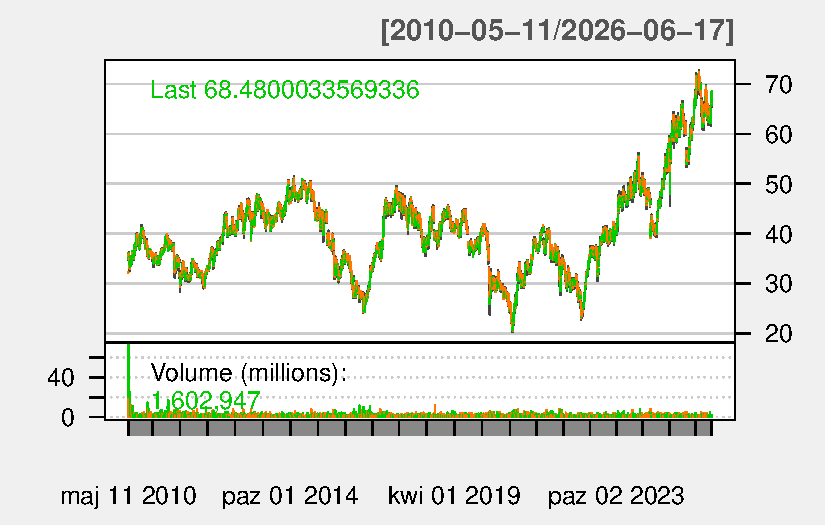
\includegraphics[keepaspectratio]{projekt2_analiza_files/figure-pdf/unnamed-chunk-7-1.pdf}}

}

\caption{Wykres akcji spółki PZU}

\end{figure}%

\subsubsection{Wskaźniki
makroekonomiczne}\label{wskaux17aniki-makroekonomiczne}

Wskaźniki makroekonomiczne zostały pobrane ze strony \textbf{GUS}
(Główny Urząd Statystyczny) i pliku \textbf{Kwartalne wskaźniki
makroekonomiczne} lub \textbf{Wybrane miesięczne wskaźniki
makroekonomiczne} {(Główny Urząd Statystyczny (2026))}.

\begin{itemize}
\tightlist
\item
  PKB pobrano z danych kwartalnych z arkusza \textbf{RACHUNKI NARODOWE}.
\item
  Inflacje pobrano z danych miesięcznych z arkusza \textbf{WSKAŹNIKI
  CEN}.
\item
  Procentową stopę bezrobocia pobrano z danych miesięcznych z arkusza
  \textbf{RYNEK PRACY}.
\end{itemize}

Te dane zostały następnie przerobione ręcznie do pliku
\textbf{makro.xlsx} do arkuszy o odpowiednich nazwach.

\begin{Shaded}
\begin{Highlighting}[]
\CommentTok{\# Autor: Maciej Kuchcik}

\NormalTok{pkb\_raw }\OtherTok{\textless{}{-}} \FunctionTok{read\_excel}\NormalTok{(}\StringTok{"makro.xlsx"}\NormalTok{, }\AttributeTok{sheet =} \StringTok{"PKB"}\NormalTok{)}

\NormalTok{rok}\OtherTok{\textless{}{-}}\FunctionTok{as.numeric}\NormalTok{(}\FunctionTok{format}\NormalTok{( }\FunctionTok{min}\NormalTok{(}\FunctionTok{as.Date}\NormalTok{(pkb\_raw}\SpecialCharTok{$}\NormalTok{DATA)), }\StringTok{"\%Y"}\NormalTok{))}
\NormalTok{kwartal}\OtherTok{\textless{}{-}}\NormalTok{(}\FunctionTok{as.numeric}\NormalTok{(}\FunctionTok{format}\NormalTok{( }\FunctionTok{min}\NormalTok{(}\FunctionTok{as.Date}\NormalTok{(pkb\_raw}\SpecialCharTok{$}\NormalTok{DATA)),}\StringTok{"\%m"}\NormalTok{)) }\SpecialCharTok{{-}} \DecValTok{1}\NormalTok{) }\SpecialCharTok{\%/\%} \DecValTok{3} \SpecialCharTok{+} \DecValTok{1}

\NormalTok{pkb\_ts }\OtherTok{\textless{}{-}} \FunctionTok{ts}\NormalTok{(}\FunctionTok{as.numeric}\NormalTok{(}\FunctionTok{as.character}\NormalTok{(pkb\_raw}\SpecialCharTok{$}\NormalTok{WARTOŚĆ)), }
             \AttributeTok{frequency =} \DecValTok{4}\NormalTok{, }\AttributeTok{start =} \FunctionTok{c}\NormalTok{(rok, kwartal))}
\FunctionTok{rysuj\_makro\_wykres}\NormalTok{(pkb\_ts}\SpecialCharTok{/}\DecValTok{1000}\NormalTok{, }\StringTok{"Produkt Krajowy Brutto Polski"}\NormalTok{, }
                   \StringTok{"Wartość (mln zł)"}\NormalTok{, FORMAT)}
\end{Highlighting}
\end{Shaded}

\begin{figure}[H]

{\centering \pandocbounded{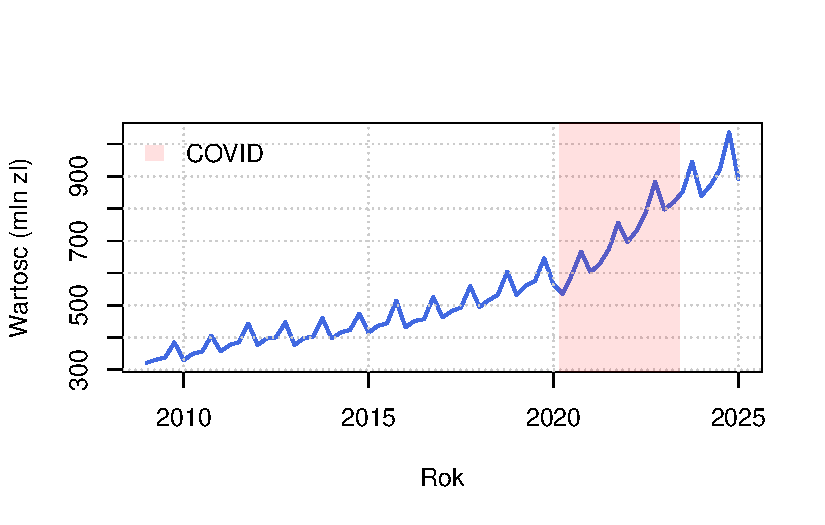
\includegraphics[keepaspectratio]{projekt2_analiza_files/figure-pdf/unnamed-chunk-8-1.pdf}}

}

\caption{Produkt Krajowy Brutto Polski}

\end{figure}%

\begin{Shaded}
\begin{Highlighting}[]
\CommentTok{\# Autor: Maciej Kuchcik}

\NormalTok{inflacja\_raw }\OtherTok{\textless{}{-}} \FunctionTok{read\_excel}\NormalTok{(}\StringTok{"makro.xlsx"}\NormalTok{, }\AttributeTok{sheet =} \StringTok{"Inflacja"}\NormalTok{)}

\NormalTok{rok}\OtherTok{\textless{}{-}}\FunctionTok{as.numeric}\NormalTok{(}\FunctionTok{format}\NormalTok{( }\FunctionTok{min}\NormalTok{(}\FunctionTok{as.Date}\NormalTok{(inflacja\_raw}\SpecialCharTok{$}\NormalTok{DATA)), }\StringTok{"\%Y"}\NormalTok{))}
\NormalTok{miesiac}\OtherTok{\textless{}{-}}\FunctionTok{as.numeric}\NormalTok{(}\FunctionTok{format}\NormalTok{( }\FunctionTok{min}\NormalTok{(}\FunctionTok{as.Date}\NormalTok{(inflacja\_raw}\SpecialCharTok{$}\NormalTok{DATA)),}\StringTok{"\%m"}\NormalTok{))}

\NormalTok{inflacja\_ts }\OtherTok{\textless{}{-}} \FunctionTok{ts}\NormalTok{(}\FunctionTok{as.numeric}\NormalTok{(}\FunctionTok{as.character}\NormalTok{(inflacja\_raw}\SpecialCharTok{$}\NormalTok{WARTOŚĆ)), }
                  \AttributeTok{frequency =} \DecValTok{12}\NormalTok{, }\AttributeTok{start =} \FunctionTok{c}\NormalTok{(rok, miesiac))}
\FunctionTok{rysuj\_makro\_wykres}\NormalTok{(inflacja\_ts }\SpecialCharTok{{-}} \DecValTok{100}\NormalTok{, }\StringTok{"Inflacja"}\NormalTok{, }\StringTok{"Inflacja \%"}\NormalTok{, FORMAT)}
\end{Highlighting}
\end{Shaded}

\begin{figure}[H]

{\centering \pandocbounded{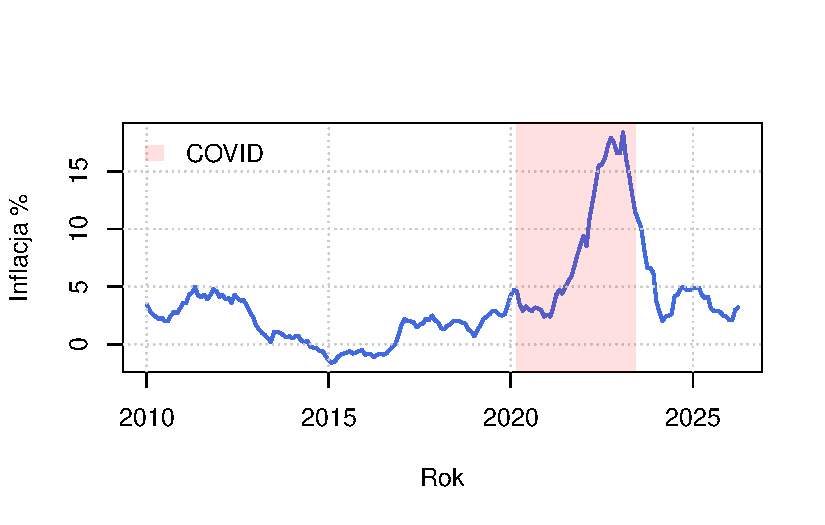
\includegraphics[keepaspectratio]{projekt2_analiza_files/figure-pdf/unnamed-chunk-9-1.pdf}}

}

\caption{Inflacja}

\end{figure}%

\begin{Shaded}
\begin{Highlighting}[]
\CommentTok{\# Autor: Maciej Kuchcik}

\NormalTok{bezrobocie\_raw }\OtherTok{\textless{}{-}} \FunctionTok{read\_excel}\NormalTok{(}\StringTok{"makro.xlsx"}\NormalTok{, }\AttributeTok{sheet =} \StringTok{"Bezrobocie\%"}\NormalTok{)}

\NormalTok{rok}\OtherTok{\textless{}{-}}\FunctionTok{as.numeric}\NormalTok{(}\FunctionTok{format}\NormalTok{( }\FunctionTok{min}\NormalTok{(}\FunctionTok{as.Date}\NormalTok{(bezrobocie\_raw}\SpecialCharTok{$}\NormalTok{DATA)), }\StringTok{"\%Y"}\NormalTok{))}
\NormalTok{miesiac}\OtherTok{\textless{}{-}}\NormalTok{(}\FunctionTok{as.numeric}\NormalTok{(}\FunctionTok{format}\NormalTok{( }\FunctionTok{min}\NormalTok{(}\FunctionTok{as.Date}\NormalTok{(bezrobocie\_raw}\SpecialCharTok{$}\NormalTok{DATA)),}\StringTok{"\%m"}\NormalTok{)))}

\NormalTok{bezrobocie\_ts }\OtherTok{\textless{}{-}} \FunctionTok{ts}\NormalTok{(}\FunctionTok{as.numeric}\NormalTok{(}\FunctionTok{as.character}\NormalTok{(bezrobocie\_raw}\SpecialCharTok{$}\NormalTok{WARTOŚĆ)), }
                    \AttributeTok{frequency =} \DecValTok{12}\NormalTok{, }\AttributeTok{start =} \FunctionTok{c}\NormalTok{(rok, miesiac))}
\FunctionTok{rysuj\_makro\_wykres}\NormalTok{(}
\NormalTok{  bezrobocie\_ts, }\StringTok{"Procentowa stopa bezrobocia"}\NormalTok{, }\StringTok{"\% stopa bezrobocia"}\NormalTok{, FORMAT)}
\end{Highlighting}
\end{Shaded}

\begin{figure}[H]

{\centering \pandocbounded{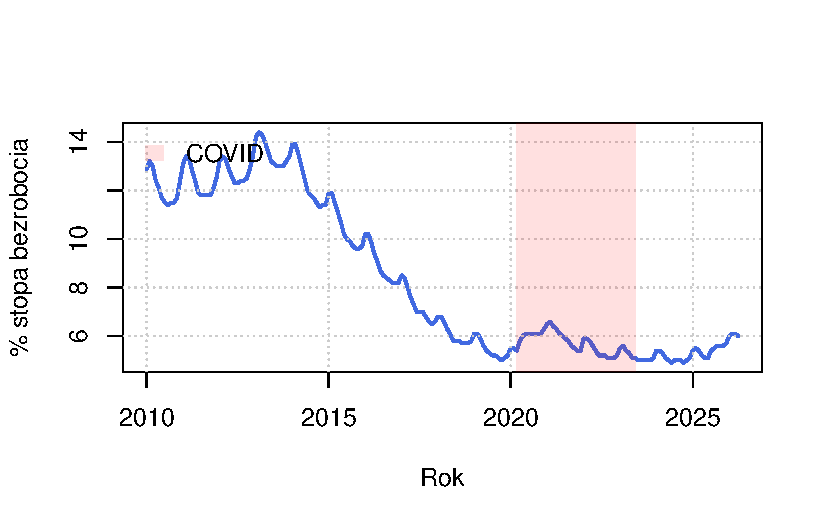
\includegraphics[keepaspectratio]{projekt2_analiza_files/figure-pdf/unnamed-chunk-10-1.pdf}}

}

\caption{Procentowa stopa bezrobocia}

\end{figure}%

\subsection{Wyznaczenie wspólnego zakresu
dat}\label{wyznaczenie-wspuxf3lnego-zakresu-dat}

Należy zbadać, czy wszystkie dane mają tą samą datę początkową i końcą.
Jeżeli ich daty się różnią, należy skrócić wszystkie zbiory do
największej z daty początkowych oraz najmniejszej z dat końcowych
(biorąc pod uwagę różne częstotliwości).

\begin{Shaded}
\begin{Highlighting}[]
\CommentTok{\# Autor: Maciej Kuchcik}

\NormalTok{zbadaj\_daty}\OtherTok{\textless{}{-}}\ControlFlowTok{function}\NormalTok{(data\_ts) \{}
\NormalTok{  min\_data }\OtherTok{\textless{}{-}} \FunctionTok{start}\NormalTok{(data\_ts)}
\NormalTok{  max\_data }\OtherTok{\textless{}{-}} \FunctionTok{end}\NormalTok{(data\_ts)}
\NormalTok{  freq }\OtherTok{\textless{}{-}} \FunctionTok{frequency}\NormalTok{(data\_ts)}
  
\NormalTok{  freq\_name }\OtherTok{\textless{}{-}} \ControlFlowTok{switch}\NormalTok{(}\FunctionTok{as.character}\NormalTok{(freq),}
                      \StringTok{"1"}  \OtherTok{=} \StringTok{"roczne"}\NormalTok{,}
                      \StringTok{"4"}  \OtherTok{=} \StringTok{"kwartalne"}\NormalTok{,}
                      \StringTok{"12"} \OtherTok{=} \StringTok{"miesięczne"}\NormalTok{,}
                      \StringTok{"52"} \OtherTok{=} \StringTok{"tygodniowe"}\NormalTok{,}
                      \StringTok{"dzienne"}\NormalTok{)}


\FunctionTok{cat}\NormalTok{(}\FunctionTok{sprintf}\NormalTok{(}
  \StringTok{"Szereg czasowy \textquotesingle{}\%s\textquotesingle{} trwa od \%d{-}\%02d do \%d{-}\%02d o częstotliwości: \%s."}\NormalTok{,}
              \FunctionTok{deparse}\NormalTok{(}\FunctionTok{substitute}\NormalTok{(data\_ts)), }
\NormalTok{              min\_data[}\DecValTok{1}\NormalTok{], min\_data[}\DecValTok{2}\NormalTok{], }
\NormalTok{              max\_data[}\DecValTok{1}\NormalTok{], max\_data[}\DecValTok{2}\NormalTok{], }
\NormalTok{              freq\_name), }\StringTok{"}\SpecialCharTok{\textbackslash{}n}\StringTok{"}\NormalTok{)}
\NormalTok{\}}

\FunctionTok{cat}\NormalTok{(}\FunctionTok{sprintf}\NormalTok{(}
  \StringTok{"Dane giełdowe PZU obejmują zakres od \%s do \%s o częstotliwości: dzienne."}\NormalTok{,}
            \FunctionTok{as.character}\NormalTok{(}\FunctionTok{index}\NormalTok{(}\FunctionTok{first}\NormalTok{(pzu\_raw))), }
            \FunctionTok{as.character}\NormalTok{(}\FunctionTok{index}\NormalTok{(}\FunctionTok{last}\NormalTok{(pzu\_raw)))), }\StringTok{"}\SpecialCharTok{\textbackslash{}n}\StringTok{"}\NormalTok{)}
\end{Highlighting}
\end{Shaded}

\begin{verbatim}
Dane giełdowe PZU obejmują zakres od 2010-05-11 do 2026-06-17 o częstotliwości: dzienne. 
\end{verbatim}

\begin{Shaded}
\begin{Highlighting}[]
\FunctionTok{zbadaj\_daty}\NormalTok{(pkb\_ts)}
\end{Highlighting}
\end{Shaded}

\begin{verbatim}
Szereg czasowy 'pkb_ts' trwa od 2009-01 do 2025-01 o częstotliwości: kwartalne. 
\end{verbatim}

\begin{Shaded}
\begin{Highlighting}[]
\FunctionTok{zbadaj\_daty}\NormalTok{(bezrobocie\_ts)}
\end{Highlighting}
\end{Shaded}

\begin{verbatim}
Szereg czasowy 'bezrobocie_ts' trwa od 2010-01 do 2026-04 o częstotliwości: miesięczne. 
\end{verbatim}

\begin{Shaded}
\begin{Highlighting}[]
\FunctionTok{zbadaj\_daty}\NormalTok{(inflacja\_ts)}
\end{Highlighting}
\end{Shaded}

\begin{verbatim}
Szereg czasowy 'inflacja_ts' trwa od 2010-01 do 2026-04 o częstotliwości: miesięczne. 
\end{verbatim}

Początki: 2010-05-11, 2009-01, 2010-01, 2010-01.

\begin{itemize}
\tightlist
\item
  Najpóźniejszy start to \textbf{2010-05-11}. Ze względu na szereg
  kwartalny, musimy zaokrąglić to do najbliższego pełnego okresu:
  \textbf{2010-07-01} (początek trzeciego kwartału).
\end{itemize}

Końce: 2026-06-12, 2025-01, 2026-04, 2026-04.

\begin{itemize}
\tightlist
\item
  Najwcześniejszy koniec to \textbf{2025-01}. Ze względu na to, że to
  szereg kwartalny, możemy brać daty aż do końca tego kwartału:
  \textbf{2025-03-31}.
\end{itemize}

\begin{Shaded}
\begin{Highlighting}[]
\CommentTok{\# Autor: Maciej Kuchcik}

\NormalTok{przytnij\_dane }\OtherTok{\textless{}{-}} \ControlFlowTok{function}\NormalTok{(data) \{}
\NormalTok{  start }\OtherTok{\textless{}{-}} \FunctionTok{as.Date}\NormalTok{(}\StringTok{"2010{-}07{-}01"}\NormalTok{)}
\NormalTok{  end   }\OtherTok{\textless{}{-}} \FunctionTok{as.Date}\NormalTok{(}\StringTok{"2025{-}03{-}31"}\NormalTok{)}
\NormalTok{  dane\_xts }\OtherTok{\textless{}{-}} \FunctionTok{as.xts}\NormalTok{(data)}
  \FunctionTok{index}\NormalTok{(dane\_xts) }\OtherTok{\textless{}{-}} \FunctionTok{as.Date}\NormalTok{(}\FunctionTok{index}\NormalTok{(dane\_xts))}
  \FunctionTok{window}\NormalTok{(dane\_xts, }\AttributeTok{start =}\NormalTok{ start, }\AttributeTok{end =}\NormalTok{ end)}
\NormalTok{\}}

\NormalTok{pkb\_final        }\OtherTok{\textless{}{-}} \FunctionTok{przytnij\_dane}\NormalTok{(pkb\_ts)}
\NormalTok{bezrobocie\_final }\OtherTok{\textless{}{-}} \FunctionTok{przytnij\_dane}\NormalTok{(bezrobocie\_ts)}
\NormalTok{inflacja\_final   }\OtherTok{\textless{}{-}} \FunctionTok{przytnij\_dane}\NormalTok{(inflacja\_ts)}
\NormalTok{pzu\_final        }\OtherTok{\textless{}{-}} \FunctionTok{przytnij\_dane}\NormalTok{(pzu\_raw)}
\end{Highlighting}
\end{Shaded}

\subsection{Synchronizacja danych}\label{synchronizacja-danych}

\begin{Shaded}
\begin{Highlighting}[]
\CommentTok{\# Autor: Maciej Kuchcik}

\NormalTok{synchronizuj\_z\_gielda }\OtherTok{\textless{}{-}} \ControlFlowTok{function}\NormalTok{(macro\_xts, target\_index) \{}
  \CommentTok{\# 1. merge z pustym (aby zachowac ilosc)}
  \CommentTok{\# 2. wypelniamy locf, zeby zachowac ostatnia wartosc}
  \CommentTok{\# 3. filtrjemy przez target (dni w gieldzie{-}nie dziala np w weekendy)}
  \FunctionTok{return}\NormalTok{(}\FunctionTok{na.locf}\NormalTok{(}\FunctionTok{merge}\NormalTok{(macro\_xts, }\FunctionTok{xts}\NormalTok{(}\AttributeTok{order.by =}\NormalTok{ target\_index)))[target\_index])}
\NormalTok{\}}
\NormalTok{index }\OtherTok{\textless{}{-}} \FunctionTok{index}\NormalTok{(pzu\_final)}

\NormalTok{pkb\_daily        }\OtherTok{\textless{}{-}} \FunctionTok{synchronizuj\_z\_gielda}\NormalTok{(pkb\_final, index)}
\NormalTok{bezrobocie\_daily }\OtherTok{\textless{}{-}} \FunctionTok{synchronizuj\_z\_gielda}\NormalTok{(bezrobocie\_final, index)}
\NormalTok{inflacja\_daily   }\OtherTok{\textless{}{-}} \FunctionTok{synchronizuj\_z\_gielda}\NormalTok{(inflacja\_final, index)}

\FunctionTok{c}\NormalTok{(}\FunctionTok{nrow}\NormalTok{(pkb\_daily), }\FunctionTok{nrow}\NormalTok{(bezrobocie\_daily), }
  \FunctionTok{nrow}\NormalTok{(inflacja\_daily), }\FunctionTok{nrow}\NormalTok{(pzu\_final))}
\end{Highlighting}
\end{Shaded}

\begin{verbatim}
[1] 3786 3786 3786 3786
\end{verbatim}

\begin{Shaded}
\begin{Highlighting}[]
\CommentTok{\# Autor: Maciej Kuchcik}

\NormalTok{all\_data }\OtherTok{\textless{}{-}} \FunctionTok{merge}\NormalTok{(pzu\_final, pkb\_daily, bezrobocie\_daily, inflacja\_daily)}
\FunctionTok{names}\NormalTok{(all\_data) }\OtherTok{\textless{}{-}} \FunctionTok{c}\NormalTok{(}\StringTok{"PZU.WA.Open"}\NormalTok{, }\StringTok{"PZU.WA.High"}\NormalTok{, }\StringTok{"PZU.WA.Low"}\NormalTok{, }
                     \StringTok{"PZU.WA.Close"}\NormalTok{, }\StringTok{"PZU.WA.Volume"}\NormalTok{, }\StringTok{"PZU.WA.Adjusted"}\NormalTok{, }
                     \StringTok{"PKB"}\NormalTok{, }\StringTok{"Bezrobocie"}\NormalTok{,}\StringTok{"Inflacja"}\NormalTok{)}
\FunctionTok{class}\NormalTok{(all\_data)}
\end{Highlighting}
\end{Shaded}

\begin{verbatim}
[1] "xts" "zoo"
\end{verbatim}

\begin{Shaded}
\begin{Highlighting}[]
\FunctionTok{head}\NormalTok{(all\_data)}
\end{Highlighting}
\end{Shaded}

\begin{verbatim}
           PZU.WA.Open PZU.WA.High PZU.WA.Low PZU.WA.Close PZU.WA.Volume
2010-07-01       35.00       35.77      34.82        35.60       2284080
2010-07-02       35.28       36.00      35.28        35.40       1717140
2010-07-05       35.42       35.52      35.20        35.21        241000
2010-07-06       35.28       35.86      35.26        35.86        468870
2010-07-07       35.41       35.90      35.35        35.80       2073780
2010-07-08       36.00       36.48      35.60        35.89       4223670
           PZU.WA.Adjusted      PKB Bezrobocie Inflacja
2010-07-01        14.04981 356417.9       11.5      102
2010-07-02        13.97087 356417.9       11.5      102
2010-07-05        13.89589 356417.9       11.5      102
2010-07-06        14.15242 356417.9       11.5      102
2010-07-07        14.12874 356417.9       11.5      102
2010-07-08        14.16425 356417.9       11.5      102
\end{verbatim}

\subsection{Podział danych na zbiór treningowy i
testowy}\label{podziaux142-danych-na-zbiuxf3r-treningowy-i-testowy}

W analizie szeregów czasowych (VAR, ARIMA) standardem jest podział na
próbę \textbf{wewnątrzpróbkową} (\emph{in-sample}, treningową) oraz
\textbf{pozapróbkową} (\emph{out-of-sample}, testową). Wszystkie modele
porównujemy uczciwie na tym samym zbiorze testowym.

Dane dzielimy chronologicznie w proporcji \textbf{80/20}:

\begin{itemize}
\tightlist
\item
  \textbf{Treningowy (80\%)} - estymacja modeli (\emph{in-sample}),
\item
  \textbf{Testowy (20\%)} - ocena jakości predykcji pozapróbkowej
  (\emph{out-of-sample}).
\end{itemize}

\begin{Shaded}
\begin{Highlighting}[]
\CommentTok{\# Autor: Maciej Kuchcik}

\NormalTok{n }\OtherTok{\textless{}{-}} \FunctionTok{nrow}\NormalTok{(all\_data)}

\NormalTok{n\_train }\OtherTok{\textless{}{-}} \FunctionTok{floor}\NormalTok{(}\FloatTok{0.80} \SpecialCharTok{*}\NormalTok{ n)}
\NormalTok{n\_test  }\OtherTok{\textless{}{-}}\NormalTok{ n }\SpecialCharTok{{-}}\NormalTok{ n\_train}

\NormalTok{all\_data\_train }\OtherTok{\textless{}{-}}\NormalTok{ all\_data[}\DecValTok{1}\SpecialCharTok{:}\NormalTok{n\_train, ]}
\NormalTok{all\_data\_test  }\OtherTok{\textless{}{-}}\NormalTok{ all\_data[(n\_train }\SpecialCharTok{+} \DecValTok{1}\NormalTok{)}\SpecialCharTok{:}\NormalTok{n, ]}

\FunctionTok{cat}\NormalTok{(}\FunctionTok{sprintf}\NormalTok{(}
  \StringTok{"Liczba obserwacji: \%d}
\StringTok{    Treningowy (80\%\%): \%d  (\%s {-} \%s)}
\StringTok{    Testowy    (20\%\%): \%d  (\%s {-} \%s)}\SpecialCharTok{\textbackslash{}n}\StringTok{"}\NormalTok{,}
\NormalTok{  n,}
  \FunctionTok{nrow}\NormalTok{(all\_data\_train), }\FunctionTok{as.character}\NormalTok{(}\FunctionTok{index}\NormalTok{(}\FunctionTok{first}\NormalTok{(all\_data\_train))),}
    \FunctionTok{as.character}\NormalTok{(}\FunctionTok{index}\NormalTok{(}\FunctionTok{last}\NormalTok{(all\_data\_train))),}
  \FunctionTok{nrow}\NormalTok{(all\_data\_test),  }\FunctionTok{as.character}\NormalTok{(}\FunctionTok{index}\NormalTok{(}\FunctionTok{first}\NormalTok{(all\_data\_test))),}
    \FunctionTok{as.character}\NormalTok{(}\FunctionTok{index}\NormalTok{(}\FunctionTok{last}\NormalTok{(all\_data\_test)))}
\NormalTok{))}
\end{Highlighting}
\end{Shaded}

\begin{verbatim}
Liczba obserwacji: 3786
    Treningowy (80%): 3028  (2010-07-01 - 2022-03-18)
    Testowy    (20%): 758  (2022-03-21 - 2025-03-31)
\end{verbatim}

\section{Analiza i predykcja}\label{analiza-i-predykcja}

Ta częśc projektu zostanie pośwęcona ostatecznej predykcji dziennych cen
zamknięcia akcji spółki PZU wykorzystujac coraz to bardziej zaawansowane
metody, by zweryfikować, które dane i jak najbardziej wpływają na jakoś
danych wyjściowych. Zostanie zastosowana taka kolejność:

\begin{enumerate}
\def\labelenumi{\arabic{enumi}.}
\tightlist
\item
  \textbf{Model naiwny/bazowy:}
  \(\text{predykcja} = \text{wartość wczorajsza}\). Wykorzystane zostaną
  tylko dane z cen zamknięcia (jeden wymiar, jedna częstotliwość).
\item
  \textbf{Model ARIMA:} wykorzystana zostanie \emph{autoarima} na cenach
  zamknięcia (jeden wymiar, jedna częstotliwość).
\item
  \textbf{Model VAR A:} użyje funkcji \emph{VAR} oraz pełnych danych
  giełdowych z cenami zamknięcia, wolumenem, cenami minimalnymi i
  maksymalnymi (kilka wymiarów, jedna częstotliwość).
\item
  \textbf{Model VAR B:} do danych z \textbf{VAR A} dołożone zostaną dane
  makroekonomiczne (kilka wymiarów, jedna częstotliwość).
\end{enumerate}

\subsection{Model naiwny}\label{model-naiwny}

Jak opisano we \hyperref[cel]{wstępie}, model naiwny (czy też bazowy)
będzie zakładał, że \[\text{predykowana cena} = \text{cena wczorajsza}\]
Będzie to model jednowymiarowy, korzystający tylko z cen zamknięcia i
posłuży jako baseline (wartość porównawcza) do predykcji z innych
modeli.

\begin{Shaded}
\begin{Highlighting}[]
\CommentTok{\# Autor: Maciej Kuchcik}

\NormalTok{pzu\_train }\OtherTok{\textless{}{-}}\NormalTok{ all\_data\_train}\SpecialCharTok{$}\NormalTok{PZU.WA.Close}
\NormalTok{pzu\_test  }\OtherTok{\textless{}{-}}\NormalTok{ all\_data\_test}\SpecialCharTok{$}\NormalTok{PZU.WA.Close}
\DocumentationTok{\#\#| renderings: [light, dark]}
\CommentTok{\# predykcja naiwna = cena wczorajsza (lag o 1 dzień) na zbiorze testowym}
\NormalTok{pzu\_test\_pred }\OtherTok{\textless{}{-}} \FunctionTok{lag}\NormalTok{(all\_data}\SpecialCharTok{$}\NormalTok{PZU.WA.Close, }\AttributeTok{k =} \DecValTok{1}\NormalTok{)[(n\_train }\SpecialCharTok{+} \DecValTok{1}\NormalTok{)}\SpecialCharTok{:}\NormalTok{n, ]}
\NormalTok{pzu\_test\_real }\OtherTok{\textless{}{-}}\NormalTok{ pzu\_test}
\NormalTok{blad\_naiwny }\OtherTok{\textless{}{-}} \FunctionTok{as.numeric}\NormalTok{(pzu\_test\_real) }\SpecialCharTok{{-}} \FunctionTok{as.numeric}\NormalTok{(pzu\_test\_pred)}

\NormalTok{metryki\_naiwny }\OtherTok{\textless{}{-}} \FunctionTok{oblicz\_metryki}\NormalTok{(blad\_naiwny, pzu\_test\_real)}

\FunctionTok{wykres\_predykcji}\NormalTok{(}\FunctionTok{index}\NormalTok{(pzu\_test\_real), }
       \FunctionTok{as.numeric}\NormalTok{(pzu\_test\_real), }
       \FunctionTok{as.numeric}\NormalTok{(pzu\_test\_pred), }
\NormalTok{       blad\_naiwny,}
       \StringTok{"Model naiwny {-} predykcja vs rzeczywistość"}\NormalTok{, }\StringTok{"naiwna"}\NormalTok{)}
\end{Highlighting}
\end{Shaded}

\begin{figure}[H]

{\centering \pandocbounded{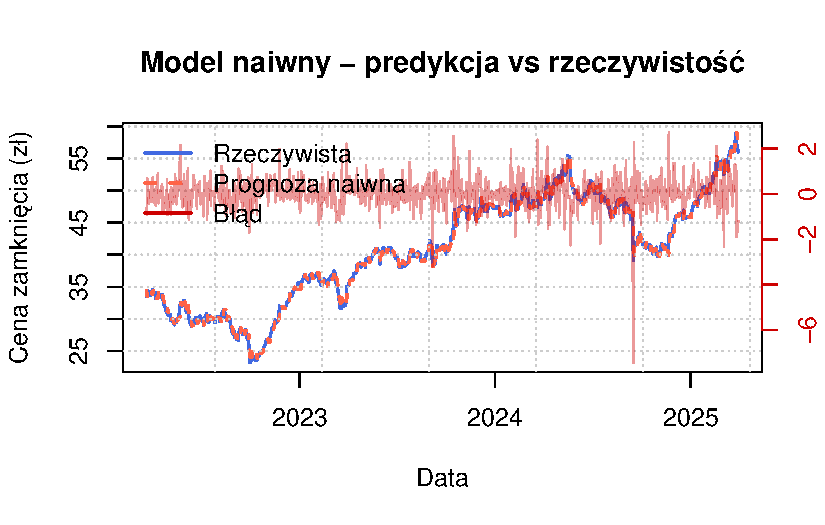
\includegraphics[keepaspectratio]{projekt2_analiza_files/figure-pdf/unnamed-chunk-16-1.pdf}}

}

\caption{Model naiwny - predykcja vs rzeczywistość (zbiór testowy)}

\end{figure}%

\begin{Shaded}
\begin{Highlighting}[]
\NormalTok{metryki\_naiwny}
\end{Highlighting}
\end{Shaded}

\begin{verbatim}
      MAE      RMSE      MAPE 
0.5220052 0.7395874 1.3100040 
\end{verbatim}

\textbf{Metryki} (zbiór testowy, ok. 3 lata: 2022-03 -- 2025-03):

\begin{itemize}
\tightlist
\item
  MAE = 0,52 zł - średnio model myli się o ok. 52 grosze,
\item
  RMSE = 0,74 zł - większy od MAE, zdarzają się pojedyncze dni z
  większymi skokami (RMSE karze mocniej za duże błędy),
\item
  MAPE = 1,31\% - procentowo błąd jest bardzo mały. Przy cenie akcji z
  zakresu ok. 23--59 zł pomyłka o 1.31\% to właśnie około pół złotego.
\end{itemize}

\textbf{Wykres:}

Linia błędu oscyluje blisko zera przez większość okresu, co potwierdza,
że ceny PZU zmieniają się powoli i model naiwny dobrze to wykorzystuje.
Widoczne są pojedyncze wyraźne skoki błędu, a największy z 16 września
2024 (ok. -7.5 zł), kolejny 6 września 2023 (ok. -3.2 zł). Okazuje się,
że to były
\href{https://strefainwestorow.pl/notowania/spolki/PLPZU0000011/dywidendy}{dni
wypłat dywidend} dla tej spółki, czego model nie mógł przewidzieć.

\subsection{Model ARIMA i ARIMAX}\label{model-arima-i-arimax}

TODO

W tej części porównane zostaną dwa modele jednowymiarowych szeregów
czasowych:

\begin{enumerate}
\def\labelenumi{\arabic{enumi}.}
\tightlist
\item
  \textbf{ARIMA} -- wykorzystujący wyłącznie wcześniejsze zmiany ceny
  zamknięcia PZU,
\item
  \textbf{ARIMAX} -- rozszerzający ARIMA o zmiany PKB, inflacji i stopy
  bezrobocia
\end{enumerate}

\begin{Shaded}
\begin{Highlighting}[]
\CommentTok{\# Autor: Andrzej Szuwald}

\CommentTok{\# Logarytmiczna stopa zwrotu ceny zamknięcia PZU}
\NormalTok{zwrot\_pzu }\OtherTok{\textless{}{-}} \FunctionTok{diff}\NormalTok{(}\FunctionTok{log}\NormalTok{(all\_data}\SpecialCharTok{$}\NormalTok{PZU.WA.Close))}

\CommentTok{\# Zmiany wskaźników makroekonomicznych}
\CommentTok{\# lag(..., k = 1) oznacza, że wykorzystujemy wartość z poprzedniego okresu sprawozdawczego. Ogranicza to ryzyko wykorzystania informacji,która nie była jeszcze znana w momencie prognozy.}

\NormalTok{pkb\_zmiana }\OtherTok{\textless{}{-}} \FunctionTok{lag}\NormalTok{(}
  \FunctionTok{diff}\NormalTok{(}\FunctionTok{log}\NormalTok{(pkb\_final)),}
  \AttributeTok{k =} \DecValTok{1}
\NormalTok{)}

\NormalTok{inflacja\_zmiana }\OtherTok{\textless{}{-}} \FunctionTok{lag}\NormalTok{(}
  \FunctionTok{diff}\NormalTok{(inflacja\_final),}
  \AttributeTok{k =} \DecValTok{1}
\NormalTok{)}

\NormalTok{bezrobocie\_zmiana }\OtherTok{\textless{}{-}} \FunctionTok{lag}\NormalTok{(}
  \FunctionTok{diff}\NormalTok{(bezrobocie\_final),}
  \AttributeTok{k =} \DecValTok{1}
\NormalTok{)}

\CommentTok{\# Przypisanie ostatniej dostępnej wartości makro do kolejnych dni giełdowych}
\NormalTok{daty\_gieldowe }\OtherTok{\textless{}{-}} \FunctionTok{index}\NormalTok{(pzu\_final)}

\NormalTok{pkb\_arimax }\OtherTok{\textless{}{-}} \FunctionTok{synchronizuj\_z\_gielda}\NormalTok{(}
\NormalTok{  pkb\_zmiana,}
\NormalTok{  daty\_gieldowe}
\NormalTok{)}

\NormalTok{inflacja\_arimax }\OtherTok{\textless{}{-}} \FunctionTok{synchronizuj\_z\_gielda}\NormalTok{(}
\NormalTok{  inflacja\_zmiana,}
\NormalTok{  daty\_gieldowe}
\NormalTok{)}

\NormalTok{bezrobocie\_arimax }\OtherTok{\textless{}{-}} \FunctionTok{synchronizuj\_z\_gielda}\NormalTok{(}
\NormalTok{  bezrobocie\_zmiana,}
\NormalTok{  daty\_gieldowe}
\NormalTok{)}

\CommentTok{\# Jeden wspólny zbiór dla obu modeli}
\NormalTok{dane\_arima\_arimax }\OtherTok{\textless{}{-}} \FunctionTok{merge}\NormalTok{(}
  \AttributeTok{zwrot =}\NormalTok{ zwrot\_pzu,}
  \AttributeTok{pkb =}\NormalTok{ pkb\_arimax,}
  \AttributeTok{inflacja =}\NormalTok{ inflacja\_arimax,}
  \AttributeTok{bezrobocie =}\NormalTok{ bezrobocie\_arimax}
\NormalTok{)}

\FunctionTok{colnames}\NormalTok{(dane\_arima\_arimax) }\OtherTok{\textless{}{-}} \FunctionTok{c}\NormalTok{(}
  \StringTok{"zwrot"}\NormalTok{,}
  \StringTok{"pkb"}\NormalTok{,}
  \StringTok{"inflacja"}\NormalTok{,}
  \StringTok{"bezrobocie"}
\NormalTok{)}

\CommentTok{\# Usunięcie braków i wartości nieskończonych}
\NormalTok{dane\_arima\_arimax }\OtherTok{\textless{}{-}}\NormalTok{ dane\_arima\_arimax[}
  \FunctionTok{apply}\NormalTok{(}
\NormalTok{    dane\_arima\_arimax,}
    \DecValTok{1}\NormalTok{,}
    \ControlFlowTok{function}\NormalTok{(wiersz) }\FunctionTok{all}\NormalTok{(}\FunctionTok{is.finite}\NormalTok{(wiersz))}
\NormalTok{  ),}
\NormalTok{]}

\CommentTok{\# Chronologiczny podział według tej samej granicy co pozostałe modele}
\NormalTok{koniec\_train }\OtherTok{\textless{}{-}} \FunctionTok{end}\NormalTok{(all\_data\_train)}

\NormalTok{dane\_arima\_train }\OtherTok{\textless{}{-}}\NormalTok{ dane\_arima\_arimax[}
  \FunctionTok{index}\NormalTok{(dane\_arima\_arimax) }\SpecialCharTok{\textless{}=}\NormalTok{ koniec\_train}
\NormalTok{]}

\NormalTok{dane\_arima\_test }\OtherTok{\textless{}{-}}\NormalTok{ dane\_arima\_arimax[}
  \FunctionTok{index}\NormalTok{(dane\_arima\_arimax) }\SpecialCharTok{\textgreater{}}\NormalTok{ koniec\_train}
\NormalTok{]}

\FunctionTok{cat}\NormalTok{(}
  \StringTok{"Trening:"}\NormalTok{,}
  \FunctionTok{nrow}\NormalTok{(dane\_arima\_train),}
  \StringTok{"obserwacji}\SpecialCharTok{\textbackslash{}n}\StringTok{"}
\NormalTok{)}
\end{Highlighting}
\end{Shaded}

\begin{verbatim}
Trening: 2896 obserwacji
\end{verbatim}

\begin{Shaded}
\begin{Highlighting}[]
\FunctionTok{cat}\NormalTok{(}
  \StringTok{"Test:"}\NormalTok{,}
  \FunctionTok{nrow}\NormalTok{(dane\_arima\_test),}
  \StringTok{"obserwacji}\SpecialCharTok{\textbackslash{}n}\StringTok{"}
\NormalTok{)}
\end{Highlighting}
\end{Shaded}

\begin{verbatim}
Test: 758 obserwacji
\end{verbatim}

\subsubsection{Standaryzacja zmiennych
makroekonomicznych}\label{standaryzacja-zmiennych-makroekonomicznych}

Przeprowadzamy standaryzacje z uwagi na to, że nasze dane mają różne
jednostki i skale

\begin{Shaded}
\begin{Highlighting}[]
\CommentTok{\# Autor: Andrzej Szuwald}

\NormalTok{y\_train }\OtherTok{\textless{}{-}} \FunctionTok{as.numeric}\NormalTok{(dane\_arima\_train}\SpecialCharTok{$}\NormalTok{zwrot)}
\NormalTok{y\_test  }\OtherTok{\textless{}{-}} \FunctionTok{as.numeric}\NormalTok{(dane\_arima\_test}\SpecialCharTok{$}\NormalTok{zwrot)}

\NormalTok{xreg\_train\_raw }\OtherTok{\textless{}{-}} \FunctionTok{as.matrix}\NormalTok{(}
\NormalTok{  dane\_arima\_train[, }\FunctionTok{c}\NormalTok{(}\StringTok{"pkb"}\NormalTok{, }\StringTok{"inflacja"}\NormalTok{, }\StringTok{"bezrobocie"}\NormalTok{)]}
\NormalTok{)}

\NormalTok{xreg\_test\_raw }\OtherTok{\textless{}{-}} \FunctionTok{as.matrix}\NormalTok{(}
\NormalTok{  dane\_arima\_test[, }\FunctionTok{c}\NormalTok{(}\StringTok{"pkb"}\NormalTok{, }\StringTok{"inflacja"}\NormalTok{, }\StringTok{"bezrobocie"}\NormalTok{)]}
\NormalTok{)}

\CommentTok{\# Parametry standaryzacji wyznaczamy tylko na treningu}
\NormalTok{xreg\_srednia }\OtherTok{\textless{}{-}} \FunctionTok{colMeans}\NormalTok{(xreg\_train\_raw)}
\NormalTok{xreg\_odchylenie }\OtherTok{\textless{}{-}} \FunctionTok{apply}\NormalTok{(xreg\_train\_raw, }\DecValTok{2}\NormalTok{, sd)}

\CommentTok{\# Zabezpieczenie przed dzieleniem przez zero}
\NormalTok{xreg\_odchylenie[}
  \SpecialCharTok{!}\FunctionTok{is.finite}\NormalTok{(xreg\_odchylenie) }\SpecialCharTok{|}\NormalTok{ xreg\_odchylenie }\SpecialCharTok{==} \DecValTok{0}
\NormalTok{] }\OtherTok{\textless{}{-}} \DecValTok{1}

\NormalTok{xreg\_train }\OtherTok{\textless{}{-}} \FunctionTok{sweep}\NormalTok{(}
\NormalTok{  xreg\_train\_raw,}
  \DecValTok{2}\NormalTok{,}
\NormalTok{  xreg\_srednia,}
  \AttributeTok{FUN =} \StringTok{"{-}"}
\NormalTok{)}

\NormalTok{xreg\_train }\OtherTok{\textless{}{-}} \FunctionTok{sweep}\NormalTok{(}
\NormalTok{  xreg\_train,}
  \DecValTok{2}\NormalTok{,}
\NormalTok{  xreg\_odchylenie,}
  \AttributeTok{FUN =} \StringTok{"/"}
\NormalTok{)}

\NormalTok{xreg\_test }\OtherTok{\textless{}{-}} \FunctionTok{sweep}\NormalTok{(}
\NormalTok{  xreg\_test\_raw,}
  \DecValTok{2}\NormalTok{,}
\NormalTok{  xreg\_srednia,}
  \AttributeTok{FUN =} \StringTok{"{-}"}
\NormalTok{)}

\NormalTok{xreg\_test }\OtherTok{\textless{}{-}} \FunctionTok{sweep}\NormalTok{(}
\NormalTok{  xreg\_test,}
  \DecValTok{2}\NormalTok{,}
\NormalTok{  xreg\_odchylenie,}
  \AttributeTok{FUN =} \StringTok{"/"}
\NormalTok{)}

\FunctionTok{colnames}\NormalTok{(xreg\_train) }\OtherTok{\textless{}{-}} \FunctionTok{c}\NormalTok{(}
  \StringTok{"pkb"}\NormalTok{,}
  \StringTok{"inflacja"}\NormalTok{,}
  \StringTok{"bezrobocie"}
\NormalTok{)}

\FunctionTok{colnames}\NormalTok{(xreg\_test) }\OtherTok{\textless{}{-}} \FunctionTok{colnames}\NormalTok{(xreg\_train)}
\end{Highlighting}
\end{Shaded}

\subsubsection{Test stacjonarności}\label{test-stacjonarnoux15bci}

\begin{Shaded}
\begin{Highlighting}[]
\CommentTok{\# Autor: Andrzej Szuwald}

\NormalTok{wynik\_adf\_arima }\OtherTok{\textless{}{-}} \FunctionTok{adf.test}\NormalTok{(y\_train)}
\end{Highlighting}
\end{Shaded}

\begin{verbatim}
Warning in adf.test(y_train): p-value smaller than printed p-value
\end{verbatim}

\begin{Shaded}
\begin{Highlighting}[]
\FunctionTok{print}\NormalTok{(wynik\_adf\_arima)}
\end{Highlighting}
\end{Shaded}

\begin{verbatim}

    Augmented Dickey-Fuller Test

data:  y_train
Dickey-Fuller = -14.513, Lag order = 14, p-value = 0.01
alternative hypothesis: stationary
\end{verbatim}

\begin{Shaded}
\begin{Highlighting}[]
\ControlFlowTok{if}\NormalTok{ (wynik\_adf\_arima}\SpecialCharTok{$}\NormalTok{p.value }\SpecialCharTok{\textless{}} \FloatTok{0.05}\NormalTok{) \{}
  \FunctionTok{cat}\NormalTok{(}
    \StringTok{"Logarytmiczne stopy zwrotu PZU są stacjonarne.}\SpecialCharTok{\textbackslash{}n}\StringTok{"}
\NormalTok{  )}
\NormalTok{\} }\ControlFlowTok{else}\NormalTok{ \{}
  \FunctionTok{cat}\NormalTok{(}
    \StringTok{"Brak podstaw do uznania stóp zwrotu za stacjonarne.}\SpecialCharTok{\textbackslash{}n}\StringTok{"}
\NormalTok{  )}
\NormalTok{\}}
\end{Highlighting}
\end{Shaded}

\begin{verbatim}
Logarytmiczne stopy zwrotu PZU są stacjonarne.
\end{verbatim}

\subsubsection{Model ARIMA}\label{model-arima}

Ponieważ zmienna została już przekształcona do postaci stacjonarnej,
ustalamy stopień różnicowania na \texttt{d\ =\ 0}. Funkcja
\texttt{auto.arima()} wybiera wartości \texttt{p} i \texttt{q} na
podstawie kryterium AICc

\begin{Shaded}
\begin{Highlighting}[]
\CommentTok{\# Autor: Andrzej Szuwald}

\NormalTok{model\_arima }\OtherTok{\textless{}{-}} \FunctionTok{auto.arima}\NormalTok{(}
\NormalTok{  y\_train,}
  \AttributeTok{d =} \DecValTok{0}\NormalTok{,}
  \AttributeTok{max.d =} \DecValTok{0}\NormalTok{,}
  \AttributeTok{stationary =} \ConstantTok{TRUE}\NormalTok{,}
  \AttributeTok{seasonal =} \ConstantTok{FALSE}\NormalTok{,}
  \AttributeTok{ic =} \StringTok{"aicc"}\NormalTok{,}
  \AttributeTok{stepwise =} \ConstantTok{FALSE}\NormalTok{,}
  \AttributeTok{approximation =} \ConstantTok{FALSE}\NormalTok{,}
  \AttributeTok{allowmean =} \ConstantTok{TRUE}
\NormalTok{)}

\FunctionTok{cat}\NormalTok{(}\StringTok{"Wybrany model ARIMA:}\SpecialCharTok{\textbackslash{}n}\StringTok{"}\NormalTok{)}
\end{Highlighting}
\end{Shaded}

\begin{verbatim}
Wybrany model ARIMA:
\end{verbatim}

\begin{Shaded}
\begin{Highlighting}[]
\FunctionTok{print}\NormalTok{(model\_arima)}
\end{Highlighting}
\end{Shaded}

\begin{verbatim}
Series: y_train 
ARIMA(0,0,0) with zero mean 

sigma^2 = 0.0002696:  log likelihood = 7791.02
AIC=-15580.03   AICc=-15580.03   BIC=-15574.06
\end{verbatim}

\begin{Shaded}
\begin{Highlighting}[]
\FunctionTok{cat}\NormalTok{(}\StringTok{"}\SpecialCharTok{\textbackslash{}n}\StringTok{Rząd modelu ARIMA:}\SpecialCharTok{\textbackslash{}n}\StringTok{"}\NormalTok{)}
\end{Highlighting}
\end{Shaded}

\begin{verbatim}

Rząd modelu ARIMA:
\end{verbatim}

\begin{Shaded}
\begin{Highlighting}[]
\FunctionTok{print}\NormalTok{(}\FunctionTok{arimaorder}\NormalTok{(model\_arima))}
\end{Highlighting}
\end{Shaded}

\begin{verbatim}
p d q 
0 0 0 
\end{verbatim}

\begin{Shaded}
\begin{Highlighting}[]
\FunctionTok{summary}\NormalTok{(model\_arima)}
\end{Highlighting}
\end{Shaded}

\begin{verbatim}
Series: y_train 
ARIMA(0,0,0) with zero mean 

sigma^2 = 0.0002696:  log likelihood = 7791.02
AIC=-15580.03   AICc=-15580.03   BIC=-15574.06

Training set error measures:
                        ME       RMSE        MAE MPE MAPE      MASE        ACF1
Training set -1.135481e-05 0.01642079 0.01175216 100  100 0.6868969 0.006895613
\end{verbatim}

\subsubsection{Model ARIMAX}\label{model-arimax}

ARIMAX rozszerza model ARIMA o zewnętrzne zmienne objaśniające:

\begin{itemize}
\tightlist
\item
  zmianę PKB,
\item
  zmianę inflacji,
\item
  zmianę stopy bezrobocia.
\end{itemize}

\begin{Shaded}
\begin{Highlighting}[]
\CommentTok{\# Autor: Andrzej Szuwald}

\NormalTok{model\_arimax }\OtherTok{\textless{}{-}} \FunctionTok{auto.arima}\NormalTok{(}
\NormalTok{  y\_train,}
  \AttributeTok{xreg =}\NormalTok{ xreg\_train,}
  \AttributeTok{d =} \DecValTok{0}\NormalTok{,}
  \AttributeTok{max.d =} \DecValTok{0}\NormalTok{,}
  \AttributeTok{stationary =} \ConstantTok{TRUE}\NormalTok{,}
  \AttributeTok{seasonal =} \ConstantTok{FALSE}\NormalTok{,}
  \AttributeTok{ic =} \StringTok{"aicc"}\NormalTok{,}
  \AttributeTok{stepwise =} \ConstantTok{FALSE}\NormalTok{,}
  \AttributeTok{approximation =} \ConstantTok{FALSE}\NormalTok{,}
  \AttributeTok{allowmean =} \ConstantTok{TRUE}
\NormalTok{)}

\FunctionTok{cat}\NormalTok{(}\StringTok{"Wybrany model ARIMAX:}\SpecialCharTok{\textbackslash{}n}\StringTok{"}\NormalTok{)}
\end{Highlighting}
\end{Shaded}

\begin{verbatim}
Wybrany model ARIMAX:
\end{verbatim}

\begin{Shaded}
\begin{Highlighting}[]
\FunctionTok{print}\NormalTok{(model\_arimax)}
\end{Highlighting}
\end{Shaded}

\begin{verbatim}
Series: y_train 
Regression with ARIMA(0,0,0) errors 

Coefficients:
        pkb  inflacja  bezrobocie
      2e-04    -6e-04      -4e-04
s.e.  4e-04     3e-04       4e-04

sigma^2 = 0.0002695:  log likelihood = 7793.27
AIC=-15578.55   AICc=-15578.53   BIC=-15554.66
\end{verbatim}

\begin{Shaded}
\begin{Highlighting}[]
\FunctionTok{cat}\NormalTok{(}\StringTok{"}\SpecialCharTok{\textbackslash{}n}\StringTok{Rząd modelu ARIMAX:}\SpecialCharTok{\textbackslash{}n}\StringTok{"}\NormalTok{)}
\end{Highlighting}
\end{Shaded}

\begin{verbatim}

Rząd modelu ARIMAX:
\end{verbatim}

\begin{Shaded}
\begin{Highlighting}[]
\FunctionTok{print}\NormalTok{(}\FunctionTok{arimaorder}\NormalTok{(model\_arimax))}
\end{Highlighting}
\end{Shaded}

\begin{verbatim}
p d q 
0 0 0 
\end{verbatim}

\begin{Shaded}
\begin{Highlighting}[]
\FunctionTok{summary}\NormalTok{(model\_arimax)}
\end{Highlighting}
\end{Shaded}

\begin{verbatim}
Series: y_train 
Regression with ARIMA(0,0,0) errors 

Coefficients:
        pkb  inflacja  bezrobocie
      2e-04    -6e-04      -4e-04
s.e.  4e-04     3e-04       4e-04

sigma^2 = 0.0002695:  log likelihood = 7793.27
AIC=-15578.55   AICc=-15578.53   BIC=-15554.66

Training set error measures:
                        ME     RMSE        MAE MPE MAPE      MASE        ACF1
Training set -1.135481e-05 0.016408 0.01176794 NaN  Inf 0.6878196 0.005823321
\end{verbatim}

\texttt{auto.arima()} wybiera model o najniższej wartości wybranego
kryterium informacyjnego spośród sprawdzanych kombinacji. W ARIMAX
zmienne makroekonomiczne są traktowane jako zewnętrzne regresory modelu

\subsubsection{Diagnostyka ARIMA}\label{diagnostyka-arima}

\begin{Shaded}
\begin{Highlighting}[]
\CommentTok{\# Autor: Andrzej Szuwald}
\FunctionTok{cat}\NormalTok{(}\StringTok{"Model\_ARIMA"}\NormalTok{)}
\end{Highlighting}
\end{Shaded}

\begin{verbatim}
Model_ARIMA
\end{verbatim}

\begin{Shaded}
\begin{Highlighting}[]
\FunctionTok{checkresiduals}\NormalTok{(model\_arima)}
\end{Highlighting}
\end{Shaded}

\begin{figure}[H]

{\centering \pandocbounded{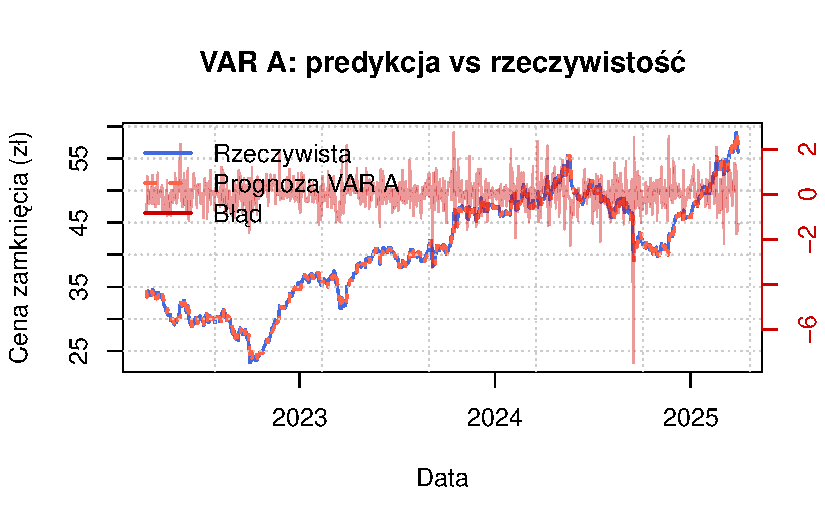
\includegraphics[keepaspectratio]{projekt2_analiza_files/figure-pdf/unnamed-chunk-22-1.pdf}}

}

\caption{Diagnostyka reszt modelu ARIMA}

\end{figure}%

\begin{verbatim}

    Ljung-Box test

data:  Residuals from ARIMA(0,0,0) with zero mean
Q* = 8.468, df = 10, p-value = 0.5832

Model df: 0.   Total lags used: 10
\end{verbatim}

\begin{Shaded}
\begin{Highlighting}[]
\FunctionTok{cat}\NormalTok{(}\StringTok{"Model\_ARIMAX"}\NormalTok{)}
\end{Highlighting}
\end{Shaded}

\begin{verbatim}
Model_ARIMAX
\end{verbatim}

\begin{Shaded}
\begin{Highlighting}[]
\FunctionTok{checkresiduals}\NormalTok{(model\_arimax)}
\end{Highlighting}
\end{Shaded}

\begin{figure}[H]

{\centering \pandocbounded{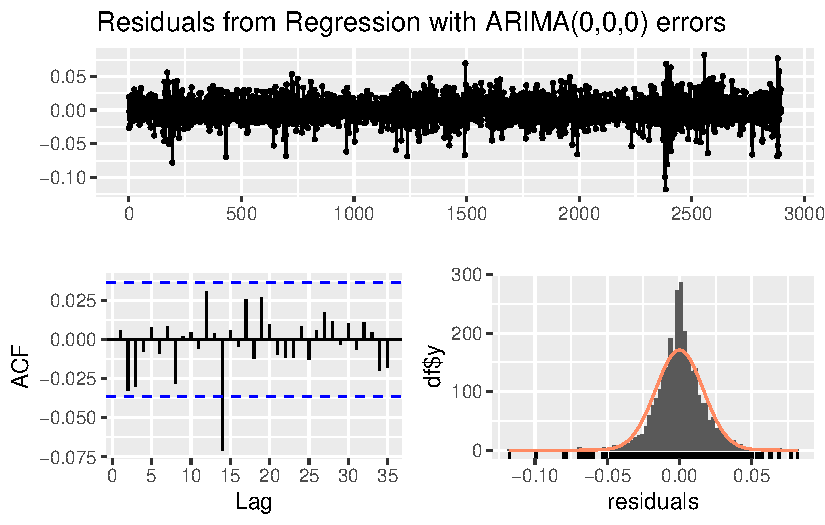
\includegraphics[keepaspectratio]{projekt2_analiza_files/figure-pdf/unnamed-chunk-22-2.pdf}}

}

\caption{Diagnostyka reszt modelu ARIMA}

\end{figure}%

\begin{verbatim}

    Ljung-Box test

data:  Residuals from Regression with ARIMA(0,0,0) errors
Q* = 8.945, df = 10, p-value = 0.5373

Model df: 0.   Total lags used: 10
\end{verbatim}

\subsubsection{Rekursywna prognoza
jednodniowa}\label{rekursywna-prognoza-jednodniowa}

Aby uczciwie porównać modele z modelem naiwnym i modelami VAR,
przeprowadzana jest prognoza jednodniowa z rozszerzanym oknem.

W każdym kroku:

\begin{enumerate}
\def\labelenumi{\arabic{enumi}.}
\tightlist
\item
  model korzysta wyłącznie z dotychczas dostępnych obserwacji,
\item
  prognozuje stopę zwrotu na kolejny dzień,
\item
  do historii dodawana jest zrealizowana wartość,
\item
  model jest ponownie estymowany.
\end{enumerate}

Struktura ARIMA(\(p,d,q\)) zostaje wybrana na treningu i nie jest
ponownie dobierana na zbiorze testowym.

\begin{Shaded}
\begin{Highlighting}[]
\CommentTok{\# Autor: Andrzej Szuwald}

\CommentTok{\# Rzędy wybranych modeli}
\NormalTok{order\_arima }\OtherTok{\textless{}{-}} \FunctionTok{unname}\NormalTok{(}
  \FunctionTok{arimaorder}\NormalTok{(model\_arima)[}\FunctionTok{c}\NormalTok{(}\StringTok{"p"}\NormalTok{, }\StringTok{"d"}\NormalTok{, }\StringTok{"q"}\NormalTok{)]}
\NormalTok{)}

\NormalTok{order\_arimax }\OtherTok{\textless{}{-}} \FunctionTok{unname}\NormalTok{(}
  \FunctionTok{arimaorder}\NormalTok{(model\_arimax)[}\FunctionTok{c}\NormalTok{(}\StringTok{"p"}\NormalTok{, }\StringTok{"d"}\NormalTok{, }\StringTok{"q"}\NormalTok{)]}
\NormalTok{)}

\CommentTok{\# Sprawdzenie, czy modele zawierają średnią}
\NormalTok{arima\_ma\_srednia }\OtherTok{\textless{}{-}}\NormalTok{ (}
  \StringTok{"intercept"} \SpecialCharTok{\%in\%} \FunctionTok{names}\NormalTok{(}\FunctionTok{coef}\NormalTok{(model\_arima))}
\NormalTok{)}

\NormalTok{arimax\_ma\_srednia }\OtherTok{\textless{}{-}}\NormalTok{ (}
  \StringTok{"intercept"} \SpecialCharTok{\%in\%} \FunctionTok{names}\NormalTok{(}\FunctionTok{coef}\NormalTok{(model\_arimax))}
\NormalTok{)}

\NormalTok{n\_test\_modeli }\OtherTok{\textless{}{-}} \FunctionTok{length}\NormalTok{(y\_test)}

\NormalTok{prognozy\_zwrot\_arima }\OtherTok{\textless{}{-}} \FunctionTok{numeric}\NormalTok{(n\_test\_modeli)}
\NormalTok{prognozy\_zwrot\_arimax }\OtherTok{\textless{}{-}} \FunctionTok{numeric}\NormalTok{(n\_test\_modeli)}

\ControlFlowTok{for}\NormalTok{ (i }\ControlFlowTok{in} \FunctionTok{seq\_len}\NormalTok{(n\_test\_modeli)) \{}

  \ControlFlowTok{if}\NormalTok{ (i }\SpecialCharTok{==} \DecValTok{1}\NormalTok{) \{}

\NormalTok{    historia\_y }\OtherTok{\textless{}{-}}\NormalTok{ y\_train}
\NormalTok{    historia\_x }\OtherTok{\textless{}{-}}\NormalTok{ xreg\_train}

\NormalTok{  \} }\ControlFlowTok{else}\NormalTok{ \{}

\NormalTok{    historia\_y }\OtherTok{\textless{}{-}} \FunctionTok{c}\NormalTok{(}
\NormalTok{      y\_train,}
\NormalTok{      y\_test[}\FunctionTok{seq\_len}\NormalTok{(i }\SpecialCharTok{{-}} \DecValTok{1}\NormalTok{)]}
\NormalTok{    )}

\NormalTok{    historia\_x }\OtherTok{\textless{}{-}} \FunctionTok{rbind}\NormalTok{(}
\NormalTok{      xreg\_train,}
\NormalTok{      xreg\_test[}\FunctionTok{seq\_len}\NormalTok{(i }\SpecialCharTok{{-}} \DecValTok{1}\NormalTok{), , }\AttributeTok{drop =} \ConstantTok{FALSE}\NormalTok{]}
\NormalTok{    )}
\NormalTok{  \}}

  \CommentTok{\# ARIMA}
\NormalTok{  model\_tmp\_arima }\OtherTok{\textless{}{-}} \FunctionTok{Arima}\NormalTok{(}
\NormalTok{    historia\_y,}
    \AttributeTok{order =}\NormalTok{ order\_arima,}
    \AttributeTok{include.mean =}\NormalTok{ arima\_ma\_srednia,}
    \AttributeTok{method =} \StringTok{"ML"}
\NormalTok{  )}

\NormalTok{  pred\_tmp\_arima }\OtherTok{\textless{}{-}} \FunctionTok{forecast}\NormalTok{(}
\NormalTok{    model\_tmp\_arima,}
    \AttributeTok{h =} \DecValTok{1}
\NormalTok{  )}

\NormalTok{  prognozy\_zwrot\_arima[i] }\OtherTok{\textless{}{-}} \FunctionTok{as.numeric}\NormalTok{(}
\NormalTok{    pred\_tmp\_arima}\SpecialCharTok{$}\NormalTok{mean[}\DecValTok{1}\NormalTok{]}
\NormalTok{  )}

  \CommentTok{\# ARIMAX}
\NormalTok{  model\_tmp\_arimax }\OtherTok{\textless{}{-}} \FunctionTok{Arima}\NormalTok{(}
\NormalTok{    historia\_y,}
    \AttributeTok{order =}\NormalTok{ order\_arimax,}
    \AttributeTok{xreg =}\NormalTok{ historia\_x,}
    \AttributeTok{include.mean =}\NormalTok{ arimax\_ma\_srednia,}
    \AttributeTok{method =} \StringTok{"ML"}
\NormalTok{  )}

\NormalTok{  xreg\_nastepny }\OtherTok{\textless{}{-}} \FunctionTok{matrix}\NormalTok{(}
\NormalTok{    xreg\_test[i, ],}
    \AttributeTok{nrow =} \DecValTok{1}
\NormalTok{  )}

  \FunctionTok{colnames}\NormalTok{(xreg\_nastepny) }\OtherTok{\textless{}{-}} \FunctionTok{colnames}\NormalTok{(xreg\_train)}

\NormalTok{  pred\_tmp\_arimax }\OtherTok{\textless{}{-}} \FunctionTok{forecast}\NormalTok{(}
\NormalTok{    model\_tmp\_arimax,}
    \AttributeTok{h =} \DecValTok{1}\NormalTok{,}
    \AttributeTok{xreg =}\NormalTok{ xreg\_nastepny}
\NormalTok{  )}

\NormalTok{  prognozy\_zwrot\_arimax[i] }\OtherTok{\textless{}{-}} \FunctionTok{as.numeric}\NormalTok{(}
\NormalTok{    pred\_tmp\_arimax}\SpecialCharTok{$}\NormalTok{mean[}\DecValTok{1}\NormalTok{]}
\NormalTok{  )}
\NormalTok{\}}
\end{Highlighting}
\end{Shaded}

\subsubsection{Odtworzenie poziomu cen}\label{odtworzenie-poziomu-cen}

Modele ARIMA i ARIMAX prognozują logarytmiczne stopy zwrotu.
Prognozowaną cenę otrzymujemy ze wzoru:

\[
\widehat{P_t} = P_{t-1}\exp(\widehat{r_t}),
\]

gdzie:

\begin{itemize}
\tightlist
\item
  \(P_{t-1}\) oznacza cenę z poprzedniego dnia,
\item
  \(\widehat{r_t}\) oznacza prognozowaną logarytmiczną stopę zwrotu.
\end{itemize}

\begin{Shaded}
\begin{Highlighting}[]
\CommentTok{\# Autor: Andrzej Szuwald}

\NormalTok{daty\_test\_modeli }\OtherTok{\textless{}{-}} \FunctionTok{index}\NormalTok{(dane\_arima\_test)}

\NormalTok{cena\_real\_modeli }\OtherTok{\textless{}{-}} \FunctionTok{as.numeric}\NormalTok{(}
\NormalTok{  all\_data}\SpecialCharTok{$}\NormalTok{PZU.WA.Close[daty\_test\_modeli]}
\NormalTok{)}

\NormalTok{cena\_poprzednia\_modeli }\OtherTok{\textless{}{-}} \FunctionTok{as.numeric}\NormalTok{(}
  \FunctionTok{lag}\NormalTok{(all\_data}\SpecialCharTok{$}\NormalTok{PZU.WA.Close, }\AttributeTok{k =} \DecValTok{1}\NormalTok{)[daty\_test\_modeli]}
\NormalTok{)}

\NormalTok{cena\_pred\_arima }\OtherTok{\textless{}{-}}\NormalTok{ cena\_poprzednia\_modeli }\SpecialCharTok{*}
  \FunctionTok{exp}\NormalTok{(prognozy\_zwrot\_arima)}

\NormalTok{cena\_pred\_arimax }\OtherTok{\textless{}{-}}\NormalTok{ cena\_poprzednia\_modeli }\SpecialCharTok{*}
  \FunctionTok{exp}\NormalTok{(prognozy\_zwrot\_arimax)}

\NormalTok{blad\_arima }\OtherTok{\textless{}{-}}\NormalTok{ cena\_real\_modeli }\SpecialCharTok{{-}}\NormalTok{ cena\_pred\_arima}
\NormalTok{blad\_arimax }\OtherTok{\textless{}{-}}\NormalTok{ cena\_real\_modeli }\SpecialCharTok{{-}}\NormalTok{ cena\_pred\_arimax}
\end{Highlighting}
\end{Shaded}

\subsubsection{Metryki modeli}\label{metryki-modeli}

\begin{Shaded}
\begin{Highlighting}[]
\CommentTok{\# Autor: Andrzej Szuwald}

\NormalTok{metryki\_arima }\OtherTok{\textless{}{-}} \FunctionTok{oblicz\_metryki}\NormalTok{(}
\NormalTok{  blad\_arima,}
\NormalTok{  cena\_real\_modeli}
\NormalTok{)}

\NormalTok{metryki\_arimax }\OtherTok{\textless{}{-}} \FunctionTok{oblicz\_metryki}\NormalTok{(}
\NormalTok{  blad\_arimax,}
\NormalTok{  cena\_real\_modeli}
\NormalTok{)}

\FunctionTok{cat}\NormalTok{(}\StringTok{"Metryki ARIMA:}\SpecialCharTok{\textbackslash{}n}\StringTok{"}\NormalTok{)}
\end{Highlighting}
\end{Shaded}

\begin{verbatim}
Metryki ARIMA:
\end{verbatim}

\begin{Shaded}
\begin{Highlighting}[]
\FunctionTok{print}\NormalTok{(metryki\_arima)}
\end{Highlighting}
\end{Shaded}

\begin{verbatim}
      MAE      RMSE      MAPE 
0.5220052 0.7395874 1.3100040 
\end{verbatim}

\begin{Shaded}
\begin{Highlighting}[]
\FunctionTok{cat}\NormalTok{(}\StringTok{"}\SpecialCharTok{\textbackslash{}n}\StringTok{Metryki ARIMAX:}\SpecialCharTok{\textbackslash{}n}\StringTok{"}\NormalTok{)}
\end{Highlighting}
\end{Shaded}

\begin{verbatim}

Metryki ARIMAX:
\end{verbatim}

\begin{Shaded}
\begin{Highlighting}[]
\FunctionTok{print}\NormalTok{(metryki\_arimax)}
\end{Highlighting}
\end{Shaded}

\begin{verbatim}
      MAE      RMSE      MAPE 
0.5222863 0.7388490 1.3100433 
\end{verbatim}

\subsubsection{Wykres ARIMA}\label{wykres-arima}

\begin{Shaded}
\begin{Highlighting}[]
\CommentTok{\# Autor: Andrzej Szuwald}

\FunctionTok{wykres\_predykcji}\NormalTok{(}
\NormalTok{  daty\_test\_modeli,}
\NormalTok{  cena\_real\_modeli,}
\NormalTok{  cena\_pred\_arima,}
\NormalTok{  blad\_arima,}
  \StringTok{"ARIMA {-} predykcja vs rzeczywistość"}\NormalTok{,}
  \StringTok{"ARIMA"}
\NormalTok{)}
\end{Highlighting}
\end{Shaded}

\begin{figure}[H]

{\centering \pandocbounded{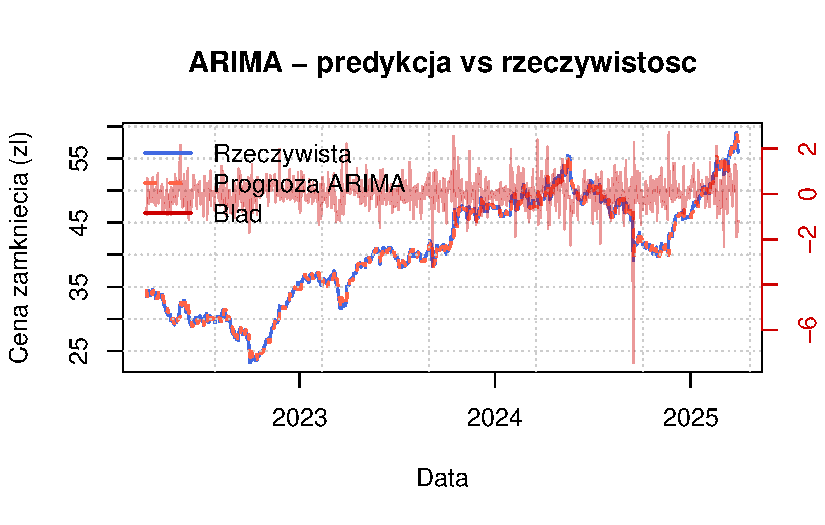
\includegraphics[keepaspectratio]{projekt2_analiza_files/figure-pdf/unnamed-chunk-26-1.pdf}}

}

\caption{ARIMA - prognoza ceny PZU na zbiorze testowym}

\end{figure}%

\subsubsection{Wykres ARIMAX}\label{wykres-arimax}

\begin{Shaded}
\begin{Highlighting}[]
\CommentTok{\# Autor: Andrzej Szuwald}

\FunctionTok{wykres\_predykcji}\NormalTok{(}
\NormalTok{  daty\_test\_modeli,}
\NormalTok{  cena\_real\_modeli,}
\NormalTok{  cena\_pred\_arimax,}
\NormalTok{  blad\_arimax,}
  \StringTok{"ARIMAX {-} predykcja vs rzeczywistość"}\NormalTok{,}
  \StringTok{"ARIMAX"}
\NormalTok{)}
\end{Highlighting}
\end{Shaded}

\begin{figure}[H]

{\centering \pandocbounded{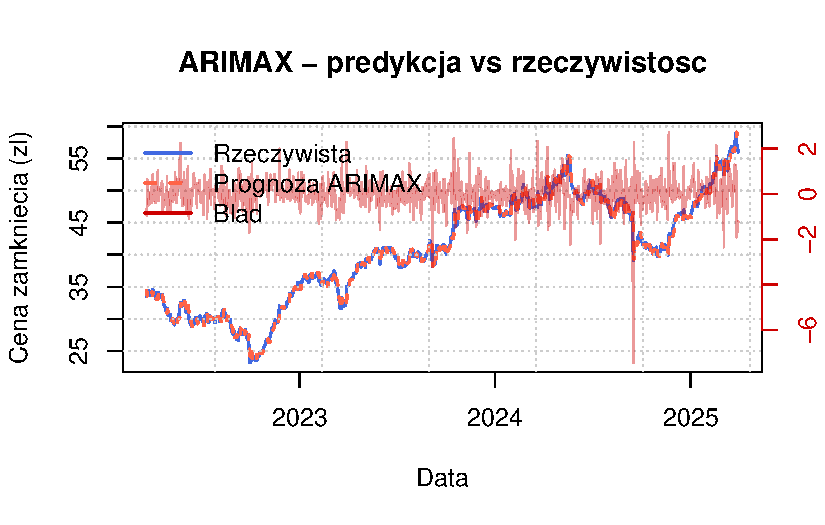
\includegraphics[keepaspectratio]{projekt2_analiza_files/figure-pdf/unnamed-chunk-27-1.pdf}}

}

\caption{ARIMAX - prognoza ceny PZU na zbiorze testowym}

\end{figure}%

\subsubsection{Porównanie ARIMA i
ARIMAX}\label{poruxf3wnanie-arima-i-arimax}

\begin{Shaded}
\begin{Highlighting}[]
\CommentTok{\# Autor: Andrzej Szuwald}

\NormalTok{tabela\_arima\_arimax }\OtherTok{\textless{}{-}} \FunctionTok{data.frame}\NormalTok{(}
  \AttributeTok{Model =} \FunctionTok{c}\NormalTok{(}\StringTok{"ARIMA"}\NormalTok{, }\StringTok{"ARIMAX"}\NormalTok{),}
  \AttributeTok{MAE =} \FunctionTok{c}\NormalTok{(}
\NormalTok{    metryki\_arima[}\StringTok{"MAE"}\NormalTok{],}
\NormalTok{    metryki\_arimax[}\StringTok{"MAE"}\NormalTok{]}
\NormalTok{  ),}
  \AttributeTok{RMSE =} \FunctionTok{c}\NormalTok{(}
\NormalTok{    metryki\_arima[}\StringTok{"RMSE"}\NormalTok{],}
\NormalTok{    metryki\_arimax[}\StringTok{"RMSE"}\NormalTok{]}
\NormalTok{  ),}
  \AttributeTok{MAPE =} \FunctionTok{c}\NormalTok{(}
\NormalTok{    metryki\_arima[}\StringTok{"MAPE"}\NormalTok{],}
\NormalTok{    metryki\_arimax[}\StringTok{"MAPE"}\NormalTok{]}
\NormalTok{  )}
\NormalTok{)}

\NormalTok{tabela\_arima\_arimax[, }\SpecialCharTok{{-}}\DecValTok{1}\NormalTok{] }\OtherTok{\textless{}{-}} \FunctionTok{round}\NormalTok{(}
\NormalTok{  tabela\_arima\_arimax[, }\SpecialCharTok{{-}}\DecValTok{1}\NormalTok{],}
  \DecValTok{3}
\NormalTok{)}

\NormalTok{knitr}\SpecialCharTok{::}\FunctionTok{kable}\NormalTok{(}
\NormalTok{  tabela\_arima\_arimax,}
  \AttributeTok{col.names =} \FunctionTok{c}\NormalTok{(}
    \StringTok{"Model"}\NormalTok{,}
    \StringTok{"MAE (zł)"}\NormalTok{,}
    \StringTok{"RMSE (zł)"}\NormalTok{,}
    \StringTok{"MAPE (\%)"}
\NormalTok{  ),}
  \AttributeTok{caption =} \StringTok{"Porównanie jakości modeli ARIMA i ARIMAX"}
\NormalTok{)}
\end{Highlighting}
\end{Shaded}

\begin{longtable}[]{@{}lrrr@{}}
\caption{Porównanie jakości modeli ARIMA i ARIMAX}\tabularnewline
\toprule\noalign{}
Model & MAE (zł) & RMSE (zł) & MAPE (\%) \\
\midrule\noalign{}
\endfirsthead
\toprule\noalign{}
Model & MAE (zł) & RMSE (zł) & MAPE (\%) \\
\midrule\noalign{}
\endhead
\bottomrule\noalign{}
\endlastfoot
ARIMA & 0.522 & 0.740 & 1.31 \\
ARIMAX & 0.522 & 0.739 & 1.31 \\
\end{longtable}

\subsection{Model VAR A}\label{model-var-a}

\subsubsection{Testy stacjonarności}\label{testy-stacjonarnoux15bci}

\begin{Shaded}
\begin{Highlighting}[]
\CommentTok{\# Autor: Maciej Kuchcik}

\NormalTok{czy\_stacjonarny }\OtherTok{\textless{}{-}} \ControlFlowTok{function}\NormalTok{(series, }\AttributeTok{nazwa =} \FunctionTok{deparse}\NormalTok{(}\FunctionTok{substitute}\NormalTok{(series))) \{}
\NormalTok{  test\_wynik }\OtherTok{\textless{}{-}} \FunctionTok{suppressWarnings}\NormalTok{(}\FunctionTok{adf.test}\NormalTok{(series))}
\NormalTok{  p }\OtherTok{\textless{}{-}}\NormalTok{ test\_wynik}\SpecialCharTok{$}\NormalTok{p.value}
\NormalTok{  p\_formatted }\OtherTok{\textless{}{-}} \ControlFlowTok{if}\NormalTok{ (p }\SpecialCharTok{\textless{}=} \FloatTok{0.01}\NormalTok{) }\StringTok{"\textless{} 0.01"} \ControlFlowTok{else} \FunctionTok{formatC}\NormalTok{(p, }\AttributeTok{digits =} \DecValTok{4}\NormalTok{, }\AttributeTok{format =} \StringTok{"f"}\NormalTok{)}
  
  \ControlFlowTok{if}\NormalTok{ (p }\SpecialCharTok{\textless{}} \FloatTok{0.05}\NormalTok{) \{}
    \FunctionTok{cat}\NormalTok{(}\FunctionTok{sprintf}\NormalTok{(}\StringTok{"\%s jest STACJONARNY (\%s).}\SpecialCharTok{\textbackslash{}n}\StringTok{"}\NormalTok{, nazwa, p\_formatted))}
    \FunctionTok{return}\NormalTok{(}\DecValTok{1}\NormalTok{)}
\NormalTok{  \} }\ControlFlowTok{else}\NormalTok{ \{}
    \FunctionTok{cat}\NormalTok{(}\FunctionTok{sprintf}\NormalTok{(}\StringTok{"\%s NIE jest stacjonarny (\%s).}\SpecialCharTok{\textbackslash{}n}\StringTok{"}\NormalTok{, nazwa, p\_formatted))}
    \FunctionTok{return}\NormalTok{(}\DecValTok{0}\NormalTok{)}
\NormalTok{  \}}
\NormalTok{\}}

\NormalTok{sprawdz\_wszystkie }\OtherTok{\textless{}{-}} \ControlFlowTok{function}\NormalTok{(data) \{}
\NormalTok{  wyniki }\OtherTok{\textless{}{-}} \FunctionTok{sapply}\NormalTok{(}\FunctionTok{names}\NormalTok{(data), }\ControlFlowTok{function}\NormalTok{(col) \{}
    \FunctionTok{czy\_stacjonarny}\NormalTok{(}\FunctionTok{na.omit}\NormalTok{(data[, col]), }\AttributeTok{nazwa =}\NormalTok{ col)}
\NormalTok{  \})}
  \FunctionTok{return}\NormalTok{(wyniki)}
\NormalTok{\}}

\FunctionTok{sprawdz\_wszystkie}\NormalTok{(all\_data\_train)}
\end{Highlighting}
\end{Shaded}

\begin{verbatim}
PZU.WA.Open NIE jest stacjonarny (0.3911).
PZU.WA.High NIE jest stacjonarny (0.4023).
PZU.WA.Low NIE jest stacjonarny (0.3936).
PZU.WA.Close NIE jest stacjonarny (0.4062).
PZU.WA.Volume jest STACJONARNY (< 0.01).
PZU.WA.Adjusted NIE jest stacjonarny (0.3707).
PKB jest STACJONARNY (< 0.01).
Bezrobocie NIE jest stacjonarny (0.6221).
Inflacja NIE jest stacjonarny (0.9900).
\end{verbatim}

\begin{verbatim}
    PZU.WA.Open     PZU.WA.High      PZU.WA.Low    PZU.WA.Close   PZU.WA.Volume 
              0               0               0               0               1 
PZU.WA.Adjusted             PKB      Bezrobocie        Inflacja 
              0               1               0               0 
\end{verbatim}

\subsubsection{Tworzenie modelu}\label{tworzenie-modelu}

Do modelu VAR(A) trafiają wyłącznie dane giełdowe (kilka wymiarów, jedna
częstotliwość). Ceny są niestacjonarne, więc każdą serię sprowadzamy do
logarytmicznych stóp zwrotu (\texttt{diff(log(...))}). Transformacje
liczymy na pełnym szeregu, a dopiero potem dzielimy na trening/test,
wtedy nie gubimy zwrotu na granicy podziału.

\begin{Shaded}
\begin{Highlighting}[]
\CommentTok{\# Autor: Maciej Kuchcik}

\NormalTok{ret\_close }\OtherTok{\textless{}{-}}\FunctionTok{diff}\NormalTok{(}\FunctionTok{log}\NormalTok{(all\_data}\SpecialCharTok{$}\NormalTok{PZU.WA.Close))}
\NormalTok{ret\_high }\OtherTok{\textless{}{-}}\FunctionTok{diff}\NormalTok{(}\FunctionTok{log}\NormalTok{(all\_data}\SpecialCharTok{$}\NormalTok{PZU.WA.High))}
\NormalTok{ret\_low }\OtherTok{\textless{}{-}}\FunctionTok{diff}\NormalTok{(}\FunctionTok{log}\NormalTok{(all\_data}\SpecialCharTok{$}\NormalTok{PZU.WA.Low))}
\NormalTok{ret\_vol }\OtherTok{\textless{}{-}} \FunctionTok{diff}\NormalTok{(}\FunctionTok{log}\NormalTok{(all\_data}\SpecialCharTok{$}\NormalTok{PZU.WA.Volume }\SpecialCharTok{+} \DecValTok{1}\NormalTok{))}

\NormalTok{dane\_var }\OtherTok{\textless{}{-}} \FunctionTok{merge}\NormalTok{(}
  \AttributeTok{zamkniecia =}\NormalTok{ ret\_close,}
  \AttributeTok{najwyzsze=}\NormalTok{ ret\_high,}
  \AttributeTok{najnizsze=}\NormalTok{ ret\_low,}
  \AttributeTok{wolumen =}\NormalTok{ret\_vol}
\NormalTok{)}

\FunctionTok{colnames}\NormalTok{(dane\_var) }\OtherTok{\textless{}{-}} \FunctionTok{c}\NormalTok{(}\StringTok{"zamkniecia"}\NormalTok{, }\StringTok{"najwyzsze"}\NormalTok{, }\StringTok{"najnizsze"}\NormalTok{, }\StringTok{"wolumen"}\NormalTok{)}

\NormalTok{dane\_var }\OtherTok{\textless{}{-}}\NormalTok{ dane\_var[}\FunctionTok{apply}\NormalTok{(dane\_var, }\DecValTok{1}\NormalTok{, }\ControlFlowTok{function}\NormalTok{(r) }\FunctionTok{all}\NormalTok{(}\FunctionTok{is.finite}\NormalTok{(r))), ]}

\CommentTok{\# podzial 80/20}
\NormalTok{koniec\_train }\OtherTok{\textless{}{-}} \FunctionTok{end}\NormalTok{(all\_data\_train)}
\NormalTok{var\_A }\OtherTok{\textless{}{-}}\NormalTok{ dane\_var[}\FunctionTok{index}\NormalTok{(dane\_var) }\SpecialCharTok{\textless{}=}\NormalTok{ koniec\_train]}
\NormalTok{var\_A\_test }\OtherTok{\textless{}{-}}\NormalTok{ dane\_var[}\FunctionTok{index}\NormalTok{(dane\_var) }\SpecialCharTok{\textgreater{}}\NormalTok{  koniec\_train]}

\NormalTok{stacjonarnosc\_var\_A }\OtherTok{\textless{}{-}} \FunctionTok{sprawdz\_wszystkie}\NormalTok{(var\_A)}
\end{Highlighting}
\end{Shaded}

\begin{verbatim}
zamkniecia jest STACJONARNY (< 0.01).
najwyzsze jest STACJONARNY (< 0.01).
najnizsze jest STACJONARNY (< 0.01).
wolumen jest STACJONARNY (< 0.01).
\end{verbatim}

\begin{Shaded}
\begin{Highlighting}[]
\ControlFlowTok{if}\NormalTok{ (}\SpecialCharTok{!}\FunctionTok{all}\NormalTok{(stacjonarnosc\_var\_A }\SpecialCharTok{==} \DecValTok{1}\NormalTok{)) \{}
  \FunctionTok{warning}\NormalTok{(}\StringTok{"Uwaga: nie wszystkie zmienne VAR(A) wyszły stacjonarne w teście ADF."}\NormalTok{)}
\NormalTok{\}}
\FunctionTok{all}\NormalTok{(stacjonarnosc\_var\_A }\SpecialCharTok{==} \DecValTok{1}\NormalTok{)}
\end{Highlighting}
\end{Shaded}

\begin{verbatim}
[1] TRUE
\end{verbatim}

\subsubsection{Predykcja}\label{predykcja}

Rząd opóźnień \(p\) dobieramy kryterium AIC.

\begin{Shaded}
\begin{Highlighting}[]
\CommentTok{\# Autor: Maciej Kuchcik}

\NormalTok{var\_A\_fit }\OtherTok{\textless{}{-}} \FunctionTok{estymuj\_var}\NormalTok{(var\_A)}
\end{Highlighting}
\end{Shaded}

\begin{verbatim}
Optymalny rząd VAR (AIC): 10 
\end{verbatim}

\begin{Shaded}
\begin{Highlighting}[]
\NormalTok{model\_var\_A }\OtherTok{\textless{}{-}}\NormalTok{ var\_A\_fit}\SpecialCharTok{$}\NormalTok{model}
\NormalTok{p\_opt       }\OtherTok{\textless{}{-}}\NormalTok{ var\_A\_fit}\SpecialCharTok{$}\NormalTok{p\_opt}
\FunctionTok{summary}\NormalTok{(model\_var\_A)}
\end{Highlighting}
\end{Shaded}

\begin{verbatim}

VAR Estimation Results:
========================= 
Endogenous variables: zamkniecia, najwyzsze, najnizsze, wolumen 
Deterministic variables: const 
Sample size: 3017 
Log Likelihood: 22276.931 
Roots of the characteristic polynomial:
0.8216 0.8216 0.7958 0.7958 0.7869 0.7869 0.7845 0.7845 0.7774 0.7774 0.775 0.775 0.7683 0.7683 0.7663 0.7663 0.7652 0.7652 0.7523 0.7523 0.7495 0.7495 0.7463 0.7463 0.7446 0.7446 0.7403 0.7403 0.7342 0.7342 0.7299 0.7238 0.7238 0.7225 0.7225 0.6478 0.6478 0.5726 0.5726 0.3382
Call:
VAR(y = dane, p = p_opt, type = "const")


Estimation results for equation zamkniecia: 
=========================================== 
zamkniecia = zamkniecia.l1 + najwyzsze.l1 + najnizsze.l1 + wolumen.l1 + zamkniecia.l2 + najwyzsze.l2 + najnizsze.l2 + wolumen.l2 + zamkniecia.l3 + najwyzsze.l3 + najnizsze.l3 + wolumen.l3 + zamkniecia.l4 + najwyzsze.l4 + najnizsze.l4 + wolumen.l4 + zamkniecia.l5 + najwyzsze.l5 + najnizsze.l5 + wolumen.l5 + zamkniecia.l6 + najwyzsze.l6 + najnizsze.l6 + wolumen.l6 + zamkniecia.l7 + najwyzsze.l7 + najnizsze.l7 + wolumen.l7 + zamkniecia.l8 + najwyzsze.l8 + najnizsze.l8 + wolumen.l8 + zamkniecia.l9 + najwyzsze.l9 + najnizsze.l9 + wolumen.l9 + zamkniecia.l10 + najwyzsze.l10 + najnizsze.l10 + wolumen.l10 + const 

                 Estimate Std. Error t value Pr(>|t|)    
zamkniecia.l1  -9.793e-02  3.729e-02  -2.626 0.008689 ** 
najwyzsze.l1    9.143e-02  4.434e-02   2.062 0.039288 *  
najnizsze.l1    7.909e-02  3.955e-02   2.000 0.045640 *  
wolumen.l1     -2.650e-04  1.242e-04  -2.134 0.032963 *  
zamkniecia.l2  -2.685e-01  6.366e-02  -4.218 2.54e-05 ***
najwyzsze.l2    2.236e-01  5.787e-02   3.863 0.000114 ***
najnizsze.l2    7.577e-02  4.977e-02   1.522 0.128025    
wolumen.l2     -2.090e-04  1.518e-04  -1.377 0.168653    
zamkniecia.l3  -3.246e-01  7.795e-02  -4.165 3.21e-05 ***
najwyzsze.l3    2.319e-01  6.511e-02   3.561 0.000375 ***
najnizsze.l3    8.138e-02  5.589e-02   1.456 0.145478    
wolumen.l3     -2.053e-04  1.694e-04  -1.211 0.225831    
zamkniecia.l4  -2.733e-01  8.546e-02  -3.198 0.001398 ** 
najwyzsze.l4    2.066e-01  6.964e-02   2.967 0.003028 ** 
najnizsze.l4    3.631e-02  5.883e-02   0.617 0.537174    
wolumen.l4     -2.620e-04  1.811e-04  -1.447 0.147990    
zamkniecia.l5  -2.217e-01  8.923e-02  -2.484 0.013040 *  
najwyzsze.l5    1.252e-01  7.202e-02   1.739 0.082197 .  
najnizsze.l5    1.033e-01  6.024e-02   1.715 0.086408 .  
wolumen.l5     -2.129e-04  1.852e-04  -1.150 0.250340    
zamkniecia.l6  -2.141e-01  8.963e-02  -2.388 0.016987 *  
najwyzsze.l6    7.956e-02  7.131e-02   1.116 0.264673    
najnizsze.l6    1.126e-01  5.984e-02   1.882 0.059911 .  
wolumen.l6     -2.261e-04  1.852e-04  -1.221 0.222282    
zamkniecia.l7  -1.569e-01  8.591e-02  -1.826 0.067921 .  
najwyzsze.l7    8.917e-02  6.824e-02   1.307 0.191424    
najnizsze.l7    6.497e-02  5.774e-02   1.125 0.260559    
wolumen.l7     -1.671e-04  1.813e-04  -0.922 0.356792    
zamkniecia.l8  -1.403e-01  7.869e-02  -1.783 0.074769 .  
najwyzsze.l8    6.949e-02  6.337e-02   1.097 0.272862    
najnizsze.l8    1.948e-02  5.341e-02   0.365 0.715335    
wolumen.l8     -3.073e-04  1.696e-04  -1.812 0.070135 .  
zamkniecia.l9  -1.964e-02  6.585e-02  -0.298 0.765537    
najwyzsze.l9   -7.320e-03  5.359e-02  -0.137 0.891373    
najnizsze.l9   -1.633e-02  4.631e-02  -0.353 0.724394    
wolumen.l9     -9.926e-05  1.520e-04  -0.653 0.513892    
zamkniecia.l10  2.773e-03  4.377e-02   0.063 0.949491    
najwyzsze.l10  -4.056e-03  3.798e-02  -0.107 0.914954    
najnizsze.l10   7.710e-03  3.488e-02   0.221 0.825069    
wolumen.l10     1.517e-04  1.244e-04   1.220 0.222603    
const          -3.111e-05  2.959e-04  -0.105 0.916277    
---
Signif. codes:  0 '***' 0.001 '**' 0.01 '*' 0.05 '.' 0.1 ' ' 1


Residual standard error: 0.01625 on 2976 degrees of freedom
Multiple R-Squared: 0.0176, Adjusted R-squared: 0.004397 
F-statistic: 1.333 on 40 and 2976 DF,  p-value: 0.07922 


Estimation results for equation najwyzsze: 
========================================== 
najwyzsze = zamkniecia.l1 + najwyzsze.l1 + najnizsze.l1 + wolumen.l1 + zamkniecia.l2 + najwyzsze.l2 + najnizsze.l2 + wolumen.l2 + zamkniecia.l3 + najwyzsze.l3 + najnizsze.l3 + wolumen.l3 + zamkniecia.l4 + najwyzsze.l4 + najnizsze.l4 + wolumen.l4 + zamkniecia.l5 + najwyzsze.l5 + najnizsze.l5 + wolumen.l5 + zamkniecia.l6 + najwyzsze.l6 + najnizsze.l6 + wolumen.l6 + zamkniecia.l7 + najwyzsze.l7 + najnizsze.l7 + wolumen.l7 + zamkniecia.l8 + najwyzsze.l8 + najnizsze.l8 + wolumen.l8 + zamkniecia.l9 + najwyzsze.l9 + najnizsze.l9 + wolumen.l9 + zamkniecia.l10 + najwyzsze.l10 + najnizsze.l10 + wolumen.l10 + const 

                 Estimate Std. Error t value Pr(>|t|)    
zamkniecia.l1   8.705e-01  2.666e-02  32.649  < 2e-16 ***
najwyzsze.l1   -7.975e-01  3.170e-02 -25.161  < 2e-16 ***
najnizsze.l1   -6.421e-02  2.828e-02  -2.271 0.023238 *  
wolumen.l1     -1.401e-04  8.878e-05  -1.578 0.114600    
zamkniecia.l2   6.683e-01  4.551e-02  14.684  < 2e-16 ***
najwyzsze.l2   -5.805e-01  4.137e-02 -14.031  < 2e-16 ***
najnizsze.l2   -2.531e-02  3.558e-02  -0.711 0.476986    
wolumen.l2     -9.651e-05  1.085e-04  -0.889 0.373970    
zamkniecia.l3   4.917e-01  5.573e-02   8.822  < 2e-16 ***
najwyzsze.l3   -5.110e-01  4.655e-02 -10.977  < 2e-16 ***
najnizsze.l3   -1.275e-02  3.996e-02  -0.319 0.749601    
wolumen.l3     -1.062e-04  1.211e-04  -0.877 0.380533    
zamkniecia.l4   4.827e-01  6.110e-02   7.901 3.85e-15 ***
najwyzsze.l4   -4.621e-01  4.978e-02  -9.282  < 2e-16 ***
najnizsze.l4   -5.623e-02  4.206e-02  -1.337 0.181309    
wolumen.l4     -5.847e-05  1.294e-04  -0.452 0.651471    
zamkniecia.l5   4.527e-01  6.379e-02   7.097 1.59e-12 ***
najwyzsze.l5   -3.984e-01  5.149e-02  -7.737 1.38e-14 ***
najnizsze.l5   -2.125e-02  4.307e-02  -0.493 0.621805    
wolumen.l5      1.474e-05  1.324e-04   0.111 0.911350    
zamkniecia.l6   3.201e-01  6.408e-02   4.996 6.20e-07 ***
najwyzsze.l6   -2.974e-01  5.098e-02  -5.833 6.03e-09 ***
najnizsze.l6   -5.745e-03  4.278e-02  -0.134 0.893182    
wolumen.l6      5.215e-06  1.324e-04   0.039 0.968590    
zamkniecia.l7   2.682e-01  6.141e-02   4.367 1.30e-05 ***
najwyzsze.l7   -2.118e-01  4.878e-02  -4.342 1.46e-05 ***
najnizsze.l7   -3.008e-02  4.128e-02  -0.729 0.466245    
wolumen.l7     -4.122e-05  1.296e-04  -0.318 0.750453    
zamkniecia.l8   1.894e-01  5.626e-02   3.367 0.000769 ***
najwyzsze.l8   -1.404e-01  4.530e-02  -3.099 0.001960 ** 
najnizsze.l8   -4.187e-02  3.818e-02  -1.097 0.272885    
wolumen.l8     -1.699e-04  1.213e-04  -1.401 0.161201    
zamkniecia.l9   1.618e-01  4.707e-02   3.437 0.000596 ***
najwyzsze.l9   -9.608e-02  3.831e-02  -2.508 0.012208 *  
najnizsze.l9   -4.411e-02  3.311e-02  -1.332 0.182864    
wolumen.l9     -7.017e-05  1.087e-04  -0.646 0.518558    
zamkniecia.l10  9.038e-02  3.129e-02   2.888 0.003905 ** 
najwyzsze.l10  -2.965e-02  2.715e-02  -1.092 0.274818    
najnizsze.l10   9.439e-03  2.493e-02   0.379 0.705065    
wolumen.l10     9.208e-05  8.891e-05   1.036 0.300453    
const          -5.756e-06  2.116e-04  -0.027 0.978293    
---
Signif. codes:  0 '***' 0.001 '**' 0.01 '*' 0.05 '.' 0.1 ' ' 1


Residual standard error: 0.01162 on 2976 degrees of freedom
Multiple R-Squared: 0.3626, Adjusted R-squared: 0.354 
F-statistic: 42.32 on 40 and 2976 DF,  p-value: < 2.2e-16 


Estimation results for equation najnizsze: 
========================================== 
najnizsze = zamkniecia.l1 + najwyzsze.l1 + najnizsze.l1 + wolumen.l1 + zamkniecia.l2 + najwyzsze.l2 + najnizsze.l2 + wolumen.l2 + zamkniecia.l3 + najwyzsze.l3 + najnizsze.l3 + wolumen.l3 + zamkniecia.l4 + najwyzsze.l4 + najnizsze.l4 + wolumen.l4 + zamkniecia.l5 + najwyzsze.l5 + najnizsze.l5 + wolumen.l5 + zamkniecia.l6 + najwyzsze.l6 + najnizsze.l6 + wolumen.l6 + zamkniecia.l7 + najwyzsze.l7 + najnizsze.l7 + wolumen.l7 + zamkniecia.l8 + najwyzsze.l8 + najnizsze.l8 + wolumen.l8 + zamkniecia.l9 + najwyzsze.l9 + najnizsze.l9 + wolumen.l9 + zamkniecia.l10 + najwyzsze.l10 + najnizsze.l10 + wolumen.l10 + const 

                 Estimate Std. Error t value Pr(>|t|)    
zamkniecia.l1   9.171e-01  2.949e-02  31.095  < 2e-16 ***
najwyzsze.l1   -1.418e-01  3.507e-02  -4.045 5.36e-05 ***
najnizsze.l1   -7.224e-01  3.128e-02 -23.093  < 2e-16 ***
wolumen.l1      3.300e-05  9.821e-05   0.336 0.736903    
zamkniecia.l2   7.237e-01  5.035e-02  14.374  < 2e-16 ***
najwyzsze.l2   -2.536e-02  4.577e-02  -0.554 0.579558    
najnizsze.l2   -6.254e-01  3.936e-02 -15.891  < 2e-16 ***
wolumen.l2      9.977e-05  1.201e-04   0.831 0.406072    
zamkniecia.l3   5.503e-01  6.165e-02   8.926  < 2e-16 ***
najwyzsze.l3    1.024e-02  5.149e-02   0.199 0.842441    
najnizsze.l3   -4.733e-01  4.420e-02 -10.709  < 2e-16 ***
wolumen.l3      1.122e-04  1.340e-04   0.837 0.402429    
zamkniecia.l4   4.667e-01  6.759e-02   6.905 6.12e-12 ***
najwyzsze.l4    4.626e-03  5.507e-02   0.084 0.933062    
najnizsze.l4   -4.543e-01  4.652e-02  -9.764  < 2e-16 ***
wolumen.l4      1.052e-05  1.432e-04   0.073 0.941439    
zamkniecia.l5   4.351e-01  7.056e-02   6.166 7.96e-10 ***
najwyzsze.l5   -4.174e-02  5.696e-02  -0.733 0.463687    
najnizsze.l5   -3.304e-01  4.764e-02  -6.936 4.92e-12 ***
wolumen.l5     -3.603e-05  1.465e-04  -0.246 0.805723    
zamkniecia.l6   3.229e-01  7.088e-02   4.555 5.45e-06 ***
najwyzsze.l6   -5.550e-02  5.640e-02  -0.984 0.325139    
najnizsze.l6   -2.283e-01  4.733e-02  -4.824 1.47e-06 ***
wolumen.l6     -4.541e-05  1.465e-04  -0.310 0.756614    
zamkniecia.l7   2.338e-01  6.794e-02   3.441 0.000587 ***
najwyzsze.l7   -6.433e-02  5.397e-02  -1.192 0.233367    
najnizsze.l7   -1.450e-01  4.566e-02  -3.175 0.001515 ** 
wolumen.l7     -4.755e-05  1.434e-04  -0.332 0.740178    
zamkniecia.l8   1.515e-01  6.223e-02   2.434 0.014984 *  
najwyzsze.l8   -3.347e-02  5.011e-02  -0.668 0.504196    
najnizsze.l8   -1.040e-01  4.224e-02  -2.462 0.013861 *  
wolumen.l8     -4.434e-05  1.341e-04  -0.331 0.741007    
zamkniecia.l9   1.428e-01  5.207e-02   2.742 0.006147 ** 
najwyzsze.l9   -6.053e-02  4.238e-02  -1.428 0.153369    
najnizsze.l9   -7.911e-02  3.663e-02  -2.160 0.030862 *  
wolumen.l9      4.621e-05  1.202e-04   0.384 0.700779    
zamkniecia.l10  8.797e-02  3.462e-02   2.541 0.011102 *  
najwyzsze.l10  -5.775e-02  3.003e-02  -1.923 0.054590 .  
najnizsze.l10  -2.998e-03  2.758e-02  -0.109 0.913459    
wolumen.l10     2.114e-04  9.836e-05   2.149 0.031693 *  
const          -2.252e-05  2.340e-04  -0.096 0.923331    
---
Signif. codes:  0 '***' 0.001 '**' 0.01 '*' 0.05 '.' 0.1 ' ' 1


Residual standard error: 0.01285 on 2976 degrees of freedom
Multiple R-Squared:  0.33,  Adjusted R-squared: 0.321 
F-statistic: 36.64 on 40 and 2976 DF,  p-value: < 2.2e-16 


Estimation results for equation wolumen: 
======================================== 
wolumen = zamkniecia.l1 + najwyzsze.l1 + najnizsze.l1 + wolumen.l1 + zamkniecia.l2 + najwyzsze.l2 + najnizsze.l2 + wolumen.l2 + zamkniecia.l3 + najwyzsze.l3 + najnizsze.l3 + wolumen.l3 + zamkniecia.l4 + najwyzsze.l4 + najnizsze.l4 + wolumen.l4 + zamkniecia.l5 + najwyzsze.l5 + najnizsze.l5 + wolumen.l5 + zamkniecia.l6 + najwyzsze.l6 + najnizsze.l6 + wolumen.l6 + zamkniecia.l7 + najwyzsze.l7 + najnizsze.l7 + wolumen.l7 + zamkniecia.l8 + najwyzsze.l8 + najnizsze.l8 + wolumen.l8 + zamkniecia.l9 + najwyzsze.l9 + najnizsze.l9 + wolumen.l9 + zamkniecia.l10 + najwyzsze.l10 + najnizsze.l10 + wolumen.l10 + const 

                Estimate Std. Error t value Pr(>|t|)    
zamkniecia.l1   -0.39029    6.08632  -0.064 0.948875    
najwyzsze.l1    11.67834    7.23617   1.614 0.106658    
najnizsze.l1    -6.52929    6.45531  -1.011 0.311878    
wolumen.l1      -0.72206    0.02027 -35.627  < 2e-16 ***
zamkniecia.l2  -10.20550   10.39005  -0.982 0.326063    
najwyzsze.l2     6.10714    9.44470   0.647 0.517928    
najnizsze.l2     5.14583    8.12214   0.634 0.526419    
wolumen.l2      -0.63920    0.02478 -25.798  < 2e-16 ***
zamkniecia.l3  -11.92972   12.72219  -0.938 0.348470    
najwyzsze.l3    -3.86541   10.62660  -0.364 0.716072    
najnizsze.l3     7.07378    9.12145   0.776 0.438099    
wolumen.l3      -0.57569    0.02765 -20.820  < 2e-16 ***
zamkniecia.l4    2.48929   13.94774   0.178 0.858364    
najwyzsze.l4   -11.01993   11.36480  -0.970 0.332297    
najnizsze.l4     0.46893    9.60079   0.049 0.961048    
wolumen.l4      -0.40827    0.02955 -13.817  < 2e-16 ***
zamkniecia.l5    7.71631   14.56162   0.530 0.596215    
najwyzsze.l5   -16.32412   11.75380  -1.389 0.164986    
najnizsze.l5     6.02996    9.83110   0.613 0.539688    
wolumen.l5      -0.29991    0.03022  -9.923  < 2e-16 ***
zamkniecia.l6    0.35706   14.62779   0.024 0.980527    
najwyzsze.l6    -5.04012   11.63848  -0.433 0.665005    
najnizsze.l6     4.01565    9.76618   0.411 0.680971    
wolumen.l6      -0.24853    0.03023  -8.221 2.98e-16 ***
zamkniecia.l7    3.69779   14.01982   0.264 0.791988    
najwyzsze.l7    -3.93692   11.13656  -0.354 0.723729    
najnizsze.l7    -0.58878    9.42318  -0.062 0.950183    
wolumen.l7      -0.20686    0.02959  -6.992 3.34e-12 ***
zamkniecia.l8    7.60928   12.84259   0.593 0.553559    
najwyzsze.l8    -2.13676   10.34141  -0.207 0.836319    
najnizsze.l8    -9.74550    8.71620  -1.118 0.263618    
wolumen.l8      -0.15915    0.02768  -5.749 9.86e-09 ***
zamkniecia.l9    5.20025   10.74611   0.484 0.628479    
najwyzsze.l9     4.88767    8.74650   0.559 0.576331    
najnizsze.l9    -9.78067    7.55835  -1.294 0.195758    
wolumen.l9      -0.08712    0.02481  -3.511 0.000453 ***
zamkniecia.l10   1.32870    7.14404   0.186 0.852467    
najwyzsze.l10   10.66584    6.19749   1.721 0.085356 .  
najnizsze.l10   -6.18827    5.69222  -1.087 0.277061    
wolumen.l10     -0.07453    0.02030  -3.672 0.000245 ***
const            0.00109    0.04829   0.023 0.981999    
---
Signif. codes:  0 '***' 0.001 '**' 0.01 '*' 0.05 '.' 0.1 ' ' 1


Residual standard error: 2.652 on 2976 degrees of freedom
Multiple R-Squared: 0.3556, Adjusted R-squared: 0.347 
F-statistic: 41.06 on 40 and 2976 DF,  p-value: < 2.2e-16 



Covariance matrix of residuals:
           zamkniecia najwyzsze  najnizsze    wolumen
zamkniecia  2.642e-04 1.497e-04  1.642e-04  6.489e-06
najwyzsze   1.497e-04 1.350e-04  9.528e-05  5.616e-03
najnizsze   1.642e-04 9.528e-05  1.652e-04 -6.260e-03
wolumen     6.489e-06 5.616e-03 -6.260e-03  7.036e+00

Correlation matrix of residuals:
           zamkniecia najwyzsze najnizsze    wolumen
zamkniecia  1.0000000    0.7928    0.7859  0.0001505
najwyzsze   0.7928142    1.0000    0.6380  0.1822207
najnizsze   0.7859351    0.6380    1.0000 -0.1836039
wolumen     0.0001505    0.1822   -0.1836  1.0000000
\end{verbatim}

Prognozę pozapróbkową budujemy rekursywnie, a model estymujemy na
zbiorze treningowym i krok po kroku dokładamy kolejne zrealizowane
obserwacje testowe, za każdym razem prognozując jeden dzień naprzód
(okno rozszerzane).

\begin{Shaded}
\begin{Highlighting}[]
\CommentTok{\# Autor: Maciej Kuchcik}

\NormalTok{prognozy }\OtherTok{\textless{}{-}} \FunctionTok{prognoza\_var\_rekursywna}\NormalTok{(}\FunctionTok{as.data.frame}\NormalTok{(var\_A), var\_A\_test, p\_opt)}
\end{Highlighting}
\end{Shaded}

Model prognozuje log-stopę zwrotu. Dzięki temu metryki są w złotówkach i
wprost porównywalne z modelem naiwnym, liczone na dokładnie tych samych
datach.

\begin{Shaded}
\begin{Highlighting}[]
\CommentTok{\# Autor: Maciej Kuchcik}

\NormalTok{daty\_test }\OtherTok{\textless{}{-}} \FunctionTok{index}\NormalTok{(var\_A\_test)}

\NormalTok{cena\_real}\OtherTok{\textless{}{-}}\FunctionTok{as.numeric}\NormalTok{(all\_data}\SpecialCharTok{$}\NormalTok{PZU.WA.Close[daty\_test])}
\NormalTok{cena\_prev}\OtherTok{\textless{}{-}}\FunctionTok{as.numeric}\NormalTok{(}\FunctionTok{lag}\NormalTok{(all\_data}\SpecialCharTok{$}\NormalTok{PZU.WA.Close, }\AttributeTok{k =} \DecValTok{1}\NormalTok{)[daty\_test])}

\NormalTok{cena\_pred\_var }\OtherTok{\textless{}{-}}\NormalTok{ cena\_prev }\SpecialCharTok{*} \FunctionTok{exp}\NormalTok{(prognozy)}
\NormalTok{e\_var }\OtherTok{\textless{}{-}}\NormalTok{ cena\_real }\SpecialCharTok{{-}}\NormalTok{ cena\_pred\_var}

\NormalTok{metryki\_var\_A }\OtherTok{\textless{}{-}} \FunctionTok{oblicz\_metryki}\NormalTok{(e\_var, cena\_real)}

\FunctionTok{cat}\NormalTok{(}\StringTok{"Metryki VAR na zbiorze testowym (zł):}\SpecialCharTok{\textbackslash{}n}\StringTok{"}\NormalTok{)}
\end{Highlighting}
\end{Shaded}

\begin{verbatim}
Metryki VAR na zbiorze testowym (zł):
\end{verbatim}

\begin{Shaded}
\begin{Highlighting}[]
\FunctionTok{print}\NormalTok{(metryki\_var\_A)}
\end{Highlighting}
\end{Shaded}

\begin{verbatim}
      MAE      RMSE      MAPE 
0.5225836 0.7396256 1.3120153 
\end{verbatim}

\begin{Shaded}
\begin{Highlighting}[]
\FunctionTok{cat}\NormalTok{(}\StringTok{"}\SpecialCharTok{\textbackslash{}n}\StringTok{Metryki modelu naiwnego na zbiorze testowym (zł):}\SpecialCharTok{\textbackslash{}n}\StringTok{"}\NormalTok{)}
\end{Highlighting}
\end{Shaded}

\begin{verbatim}

Metryki modelu naiwnego na zbiorze testowym (zł):
\end{verbatim}

\begin{Shaded}
\begin{Highlighting}[]
\FunctionTok{print}\NormalTok{(metryki\_naiwny)}
\end{Highlighting}
\end{Shaded}

\begin{verbatim}
      MAE      RMSE      MAPE 
0.5220052 0.7395874 1.3100040 
\end{verbatim}

\begin{Shaded}
\begin{Highlighting}[]
\CommentTok{\# Autor: Maciej Kuchcik}

\FunctionTok{wykres\_predykcji}\NormalTok{(daty\_test, cena\_real, cena\_pred\_var, e\_var,}
                 \StringTok{"VAR A: predykcja vs rzeczywistość"}\NormalTok{, }\StringTok{"VAR A"}\NormalTok{)}
\end{Highlighting}
\end{Shaded}

\begin{figure}[H]

{\centering \pandocbounded{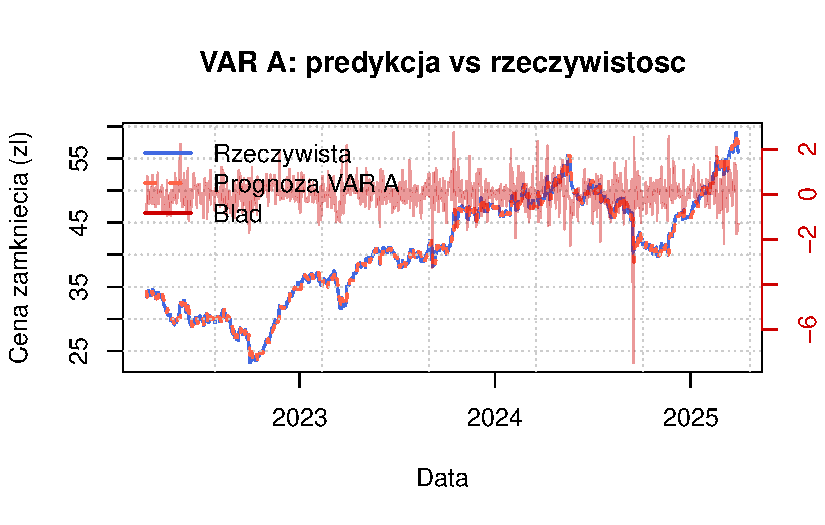
\includegraphics[keepaspectratio]{projekt2_analiza_files/figure-pdf/unnamed-chunk-34-1.pdf}}

}

\caption{VAR A: predykcja vs rzeczywistość (zbiór testowy)}

\end{figure}%

\begin{Shaded}
\begin{Highlighting}[]
\DocumentationTok{\#\#| renderings: [light, dark]}
\end{Highlighting}
\end{Shaded}

\textbf{Wynik:} VAR na samych danych giełdowych praktycznie nie różni
się od modelu naiwnego (MAE: 0,52 zł, RMSE: 0,74 zł, MAPE: 1,31\% są
prawie identycznie). Dzienne stopy zwrotu PZU są w praktyce
nieprzewidywalne na podstawie własnej historii oraz cen max/min i
wolumenu, a prognozowany zwrot oscyluje wokół zera, więc predykcja ceny
sprowadza się do \textbf{ceny wczorajszej}.

\subsection{Model VAR B}\label{model-var-b}

Model VAR B rozszerza VAR A o trzy zmienne makroekonomiczne:
\textbf{PKB} (kwartalne), \textbf{inflację} i \textbf{stopę bezrobocia}
(miesięczne). Pojawia się problem różnych częstotliwości. Dane giełdowe
są dzienne, a makro kwartalne/miesięczne.

Do tego celu użyta została funkcja schodkowa (\texttt{na.locf}), a nie
interpolacja liniowa, ponieważ lepiej odwzorowuje to informacje giełdowe
(PKB nie jest znane codziennie.)

\subsubsection{Tworzenie modelu}\label{tworzenie-modelu-1}

\begin{Shaded}
\begin{Highlighting}[]
\CommentTok{\# Autor: Maciej Kuchcik}

\NormalTok{pkb\_d\_daily }\OtherTok{\textless{}{-}} \FunctionTok{synchronizuj\_z\_gielda}\NormalTok{(}\FunctionTok{diff}\NormalTok{(}\FunctionTok{log}\NormalTok{(pkb\_final)), index)}
\NormalTok{inflacja\_d\_daily }\OtherTok{\textless{}{-}} \FunctionTok{synchronizuj\_z\_gielda}\NormalTok{(}\FunctionTok{diff}\NormalTok{(inflacja\_final), index)}
\NormalTok{bezrob\_d\_daily}\OtherTok{\textless{}{-}} \FunctionTok{synchronizuj\_z\_gielda}\NormalTok{(}\FunctionTok{diff}\NormalTok{(bezrobocie\_final),index)}


\NormalTok{dane\_var\_B }\OtherTok{\textless{}{-}} \FunctionTok{merge}\NormalTok{(}
  \AttributeTok{zamkniecia =} \FunctionTok{diff}\NormalTok{(}\FunctionTok{log}\NormalTok{(all\_data}\SpecialCharTok{$}\NormalTok{PZU.WA.Close)),}
  \AttributeTok{najwyzsze =} \FunctionTok{diff}\NormalTok{(}\FunctionTok{log}\NormalTok{(all\_data}\SpecialCharTok{$}\NormalTok{PZU.WA.High)),}
  \AttributeTok{najnizsze =} \FunctionTok{diff}\NormalTok{(}\FunctionTok{log}\NormalTok{(all\_data}\SpecialCharTok{$}\NormalTok{PZU.WA.Low)),}
  \AttributeTok{wolumen =} \FunctionTok{diff}\NormalTok{(}\FunctionTok{log}\NormalTok{(all\_data}\SpecialCharTok{$}\NormalTok{PZU.WA.Volume }\SpecialCharTok{+} \DecValTok{1}\NormalTok{)),}
  \AttributeTok{pkb =}\NormalTok{ pkb\_d\_daily,}
  \AttributeTok{bezrob=}\NormalTok{ bezrob\_d\_daily,}
  \AttributeTok{inflacja =}\NormalTok{inflacja\_d\_daily}
\NormalTok{)}

\FunctionTok{colnames}\NormalTok{(dane\_var\_B) }\OtherTok{\textless{}{-}} \FunctionTok{c}\NormalTok{(}\StringTok{"zamkniecia"}\NormalTok{, }\StringTok{"najwyzsze"}\NormalTok{, }
                    \StringTok{"najnizsze"}\NormalTok{, }\StringTok{"wolumen"}\NormalTok{,}
                    \StringTok{"pkb"}\NormalTok{, }\StringTok{"bezrob"}\NormalTok{, }\StringTok{"inflacja"}\NormalTok{)}

\NormalTok{dane\_var\_B }\OtherTok{\textless{}{-}}\NormalTok{ dane\_var\_B[}\FunctionTok{apply}\NormalTok{(dane\_var\_B, }\DecValTok{1}\NormalTok{, }
                         \ControlFlowTok{function}\NormalTok{(r) }\FunctionTok{all}\NormalTok{(}\FunctionTok{is.finite}\NormalTok{(r))), ]}

\CommentTok{\# podział 80/20}
\NormalTok{koniec\_train }\OtherTok{\textless{}{-}} \FunctionTok{end}\NormalTok{(all\_data\_train)}
\NormalTok{var\_B }\OtherTok{\textless{}{-}}\NormalTok{ dane\_var\_B[}\FunctionTok{index}\NormalTok{(dane\_var\_B) }\SpecialCharTok{\textless{}=}\NormalTok{ koniec\_train]}
\NormalTok{var\_B\_test}\OtherTok{\textless{}{-}}\NormalTok{ dane\_var\_B[}\FunctionTok{index}\NormalTok{(dane\_var\_B) }\SpecialCharTok{\textgreater{}}\NormalTok{  koniec\_train]}

\NormalTok{stacjonarnosc\_var\_B }\OtherTok{\textless{}{-}} \FunctionTok{sprawdz\_wszystkie}\NormalTok{(var\_B)}
\end{Highlighting}
\end{Shaded}

\begin{verbatim}
zamkniecia jest STACJONARNY (< 0.01).
najwyzsze jest STACJONARNY (< 0.01).
najnizsze jest STACJONARNY (< 0.01).
wolumen jest STACJONARNY (< 0.01).
pkb jest STACJONARNY (< 0.01).
bezrob jest STACJONARNY (< 0.01).
inflacja jest STACJONARNY (< 0.01).
\end{verbatim}

\begin{Shaded}
\begin{Highlighting}[]
\ControlFlowTok{if}\NormalTok{ (}\SpecialCharTok{!}\FunctionTok{all}\NormalTok{(stacjonarnosc\_var\_B }\SpecialCharTok{==} \DecValTok{1}\NormalTok{)) \{}
  \FunctionTok{warning}\NormalTok{(}\StringTok{"NIE WSZYSTKIE zmienne stacjonarne w ADF."}\NormalTok{)}
\NormalTok{\}}
\FunctionTok{all}\NormalTok{(stacjonarnosc\_var\_B }\SpecialCharTok{==} \DecValTok{1}\NormalTok{)}
\end{Highlighting}
\end{Shaded}

\begin{verbatim}
[1] TRUE
\end{verbatim}

\subsubsection{Predykcja}\label{predykcja-1}

\begin{Shaded}
\begin{Highlighting}[]
\CommentTok{\# Autor: Maciej Kuchcik}

\NormalTok{var\_B\_fit }\OtherTok{\textless{}{-}} \FunctionTok{estymuj\_var}\NormalTok{(var\_B)}
\end{Highlighting}
\end{Shaded}

\begin{verbatim}
Optymalny rząd VAR (AIC): 10 
\end{verbatim}

\begin{Shaded}
\begin{Highlighting}[]
\NormalTok{model\_var\_B }\OtherTok{\textless{}{-}}\NormalTok{ var\_B\_fit}\SpecialCharTok{$}\NormalTok{model}
\NormalTok{p\_opt\_B  }\OtherTok{\textless{}{-}}\NormalTok{ var\_B\_fit}\SpecialCharTok{$}\NormalTok{p\_opt}
\FunctionTok{summary}\NormalTok{(model\_var\_B)}
\end{Highlighting}
\end{Shaded}

\begin{verbatim}

VAR Estimation Results:
========================= 
Endogenous variables: zamkniecia, najwyzsze, najnizsze, wolumen, pkb, bezrob, inflacja 
Deterministic variables: const 
Sample size: 2952 
Log Likelihood: 36353.278 
Roots of the characteristic polynomial:
0.985 0.985 0.945 0.8178 0.8178 0.8145 0.8145 0.7979 0.7979 0.7938 0.7938 0.7931 0.7931 0.7925 0.7925 0.7827 0.7827 0.7807 0.7785 0.7785 0.7716 0.7716 0.7685 0.7685 0.7685 0.7685 0.7671 0.7671 0.7646 0.7646 0.7644 0.7644 0.7572 0.7572 0.754 0.754 0.742 0.742 0.7402 0.7402 0.7313 0.7313 0.7239 0.7239 0.7221 0.7221 0.7212 0.7212 0.7199 0.7199 0.7184 0.7184 0.7175 0.7175 0.6948 0.6948 0.6889 0.6889 0.6874 0.6874 0.6808 0.6808 0.6743 0.6743 0.6547 0.6359 0.6359 0.5897 0.5897 0.03054
Call:
VAR(y = dane, p = p_opt, type = "const")


Estimation results for equation zamkniecia: 
=========================================== 
zamkniecia = zamkniecia.l1 + najwyzsze.l1 + najnizsze.l1 + wolumen.l1 + pkb.l1 + bezrob.l1 + inflacja.l1 + zamkniecia.l2 + najwyzsze.l2 + najnizsze.l2 + wolumen.l2 + pkb.l2 + bezrob.l2 + inflacja.l2 + zamkniecia.l3 + najwyzsze.l3 + najnizsze.l3 + wolumen.l3 + pkb.l3 + bezrob.l3 + inflacja.l3 + zamkniecia.l4 + najwyzsze.l4 + najnizsze.l4 + wolumen.l4 + pkb.l4 + bezrob.l4 + inflacja.l4 + zamkniecia.l5 + najwyzsze.l5 + najnizsze.l5 + wolumen.l5 + pkb.l5 + bezrob.l5 + inflacja.l5 + zamkniecia.l6 + najwyzsze.l6 + najnizsze.l6 + wolumen.l6 + pkb.l6 + bezrob.l6 + inflacja.l6 + zamkniecia.l7 + najwyzsze.l7 + najnizsze.l7 + wolumen.l7 + pkb.l7 + bezrob.l7 + inflacja.l7 + zamkniecia.l8 + najwyzsze.l8 + najnizsze.l8 + wolumen.l8 + pkb.l8 + bezrob.l8 + inflacja.l8 + zamkniecia.l9 + najwyzsze.l9 + najnizsze.l9 + wolumen.l9 + pkb.l9 + bezrob.l9 + inflacja.l9 + zamkniecia.l10 + najwyzsze.l10 + najnizsze.l10 + wolumen.l10 + pkb.l10 + bezrob.l10 + inflacja.l10 + const 

                 Estimate Std. Error t value Pr(>|t|)    
zamkniecia.l1  -0.0868660  0.0379234  -2.291 0.022061 *  
najwyzsze.l1    0.0888195  0.0450684   1.971 0.048845 *  
najnizsze.l1    0.0660255  0.0402682   1.640 0.101188    
wolumen.l1     -0.0002477  0.0001265  -1.959 0.050262 .  
pkb.l1          0.0118120  0.0157707   0.749 0.453928    
bezrob.l1       0.0058620  0.0068468   0.856 0.391977    
inflacja.l1    -0.0009971  0.0025732  -0.387 0.698428    
zamkniecia.l2  -0.2585351  0.0649717  -3.979 7.09e-05 ***
najwyzsze.l2    0.2158319  0.0589359   3.662 0.000255 ***
najnizsze.l2    0.0696017  0.0507285   1.372 0.170157    
wolumen.l2     -0.0001893  0.0001554  -1.218 0.223232    
pkb.l2         -0.0020301  0.0218324  -0.093 0.925920    
bezrob.l2      -0.0179181  0.0095236  -1.881 0.060013 .  
inflacja.l2     0.0043313  0.0036160   1.198 0.231086    
zamkniecia.l3  -0.3108753  0.0796404  -3.903 9.70e-05 ***
najwyzsze.l3    0.2279614  0.0664754   3.429 0.000614 ***
najnizsze.l3    0.0716777  0.0570045   1.257 0.208709    
wolumen.l3     -0.0001842  0.0001736  -1.061 0.288638    
pkb.l3         -0.0163913  0.0218515  -0.750 0.453243    
bezrob.l3       0.0093607  0.0095297   0.982 0.326052    
inflacja.l3    -0.0033697  0.0036156  -0.932 0.351423    
zamkniecia.l4  -0.2513113  0.0874118  -2.875 0.004070 ** 
najwyzsze.l4    0.1923335  0.0710811   2.706 0.006854 ** 
najnizsze.l4    0.0232480  0.0601622   0.386 0.699213    
wolumen.l4     -0.0002188  0.0001860  -1.176 0.239742    
pkb.l4          0.0128207  0.0218820   0.586 0.557988    
bezrob.l4       0.0038523  0.0095248   0.404 0.685909    
inflacja.l4     0.0026273  0.0036174   0.726 0.467721    
zamkniecia.l5  -0.1964655  0.0912585  -2.153 0.031414 *  
najwyzsze.l5    0.1086581  0.0734684   1.479 0.139256    
najnizsze.l5    0.0972285  0.0615966   1.578 0.114567    
wolumen.l5     -0.0001696  0.0001906  -0.890 0.373784    
pkb.l5         -0.0178039  0.0218995  -0.813 0.416296    
bezrob.l5      -0.0077038  0.0095215  -0.809 0.418526    
inflacja.l5    -0.0016547  0.0036169  -0.457 0.647361    
zamkniecia.l6  -0.1781926  0.0916513  -1.944 0.051963 .  
najwyzsze.l6    0.0539643  0.0727040   0.742 0.457998    
najnizsze.l6    0.0948135  0.0612074   1.549 0.121479    
wolumen.l6     -0.0001924  0.0001907  -1.009 0.313155    
pkb.l6          0.0090479  0.0217984   0.415 0.678119    
bezrob.l6       0.0095900  0.0095169   1.008 0.313694    
inflacja.l6     0.0065932  0.0036244   1.819 0.069001 .  
zamkniecia.l7  -0.1116051  0.0878697  -1.270 0.204144    
najwyzsze.l7    0.0578647  0.0696114   0.831 0.405899    
najnizsze.l7    0.0518247  0.0590286   0.878 0.380039    
wolumen.l7     -0.0001511  0.0001887  -0.801 0.423319    
pkb.l7          0.0094567  0.0217786   0.434 0.664162    
bezrob.l7      -0.0066337  0.0095228  -0.697 0.486099    
inflacja.l7    -0.0078051  0.0036245  -2.153 0.031370 *  
zamkniecia.l8  -0.1108851  0.0804915  -1.378 0.168434    
najwyzsze.l8    0.0497524  0.0647161   0.769 0.442087    
najnizsze.l8    0.0128525  0.0546300   0.235 0.814021    
wolumen.l8     -0.0003356  0.0001775  -1.891 0.058698 .  
pkb.l8          0.0017181  0.0217318   0.079 0.936991    
bezrob.l8       0.0033295  0.0095135   0.350 0.726384    
inflacja.l8     0.0032690  0.0036193   0.903 0.366483    
zamkniecia.l9  -0.0029825  0.0673736  -0.044 0.964694    
najwyzsze.l9   -0.0171194  0.0547688  -0.313 0.754626    
najnizsze.l9   -0.0109866  0.0473486  -0.232 0.816526    
wolumen.l9     -0.0001066  0.0001586  -0.672 0.501622    
pkb.l9          0.0150977  0.0216377   0.698 0.485389    
bezrob.l9       0.0158437  0.0095127   1.666 0.095916 .  
inflacja.l9    -0.0006959  0.0036031  -0.193 0.846857    
zamkniecia.l10  0.0054245  0.0448363   0.121 0.903712    
najwyzsze.l10  -0.0109274  0.0387067  -0.282 0.777724    
najnizsze.l10   0.0127709  0.0355384   0.359 0.719355    
wolumen.l10     0.0001476  0.0001283   1.151 0.249894    
pkb.l10        -0.0204317  0.0156032  -1.309 0.190485    
bezrob.l10     -0.0147748  0.0068007  -2.173 0.029896 *  
inflacja.l10   -0.0017378  0.0025804  -0.673 0.500712    
const          -0.0001003  0.0003098  -0.324 0.746154    
---
Signif. codes:  0 '***' 0.001 '**' 0.01 '*' 0.05 '.' 0.1 ' ' 1


Residual standard error: 0.01631 on 2881 degrees of freedom
Multiple R-Squared: 0.0272, Adjusted R-squared: 0.003561 
F-statistic: 1.151 on 70 and 2881 DF,  p-value: 0.186 


Estimation results for equation najwyzsze: 
========================================== 
najwyzsze = zamkniecia.l1 + najwyzsze.l1 + najnizsze.l1 + wolumen.l1 + pkb.l1 + bezrob.l1 + inflacja.l1 + zamkniecia.l2 + najwyzsze.l2 + najnizsze.l2 + wolumen.l2 + pkb.l2 + bezrob.l2 + inflacja.l2 + zamkniecia.l3 + najwyzsze.l3 + najnizsze.l3 + wolumen.l3 + pkb.l3 + bezrob.l3 + inflacja.l3 + zamkniecia.l4 + najwyzsze.l4 + najnizsze.l4 + wolumen.l4 + pkb.l4 + bezrob.l4 + inflacja.l4 + zamkniecia.l5 + najwyzsze.l5 + najnizsze.l5 + wolumen.l5 + pkb.l5 + bezrob.l5 + inflacja.l5 + zamkniecia.l6 + najwyzsze.l6 + najnizsze.l6 + wolumen.l6 + pkb.l6 + bezrob.l6 + inflacja.l6 + zamkniecia.l7 + najwyzsze.l7 + najnizsze.l7 + wolumen.l7 + pkb.l7 + bezrob.l7 + inflacja.l7 + zamkniecia.l8 + najwyzsze.l8 + najnizsze.l8 + wolumen.l8 + pkb.l8 + bezrob.l8 + inflacja.l8 + zamkniecia.l9 + najwyzsze.l9 + najnizsze.l9 + wolumen.l9 + pkb.l9 + bezrob.l9 + inflacja.l9 + zamkniecia.l10 + najwyzsze.l10 + najnizsze.l10 + wolumen.l10 + pkb.l10 + bezrob.l10 + inflacja.l10 + const 

                 Estimate Std. Error t value Pr(>|t|)    
zamkniecia.l1   8.767e-01  2.710e-02  32.346  < 2e-16 ***
najwyzsze.l1   -8.008e-01  3.221e-02 -24.862  < 2e-16 ***
najnizsze.l1   -7.077e-02  2.878e-02  -2.459 0.013987 *  
wolumen.l1     -1.329e-04  9.037e-05  -1.470 0.141675    
pkb.l1         -6.977e-03  1.127e-02  -0.619 0.535941    
bezrob.l1      -4.757e-04  4.893e-03  -0.097 0.922568    
inflacja.l1    -1.426e-03  1.839e-03  -0.775 0.438293    
zamkniecia.l2   6.697e-01  4.643e-02  14.423  < 2e-16 ***
najwyzsze.l2   -5.867e-01  4.212e-02 -13.930  < 2e-16 ***
najnizsze.l2   -2.009e-02  3.625e-02  -0.554 0.579459    
wolumen.l2     -7.591e-05  1.111e-04  -0.683 0.494410    
pkb.l2          1.172e-02  1.560e-02   0.751 0.452683    
bezrob.l2      -7.483e-03  6.806e-03  -1.099 0.271690    
inflacja.l2     3.750e-03  2.584e-03   1.451 0.146820    
zamkniecia.l3   4.896e-01  5.692e-02   8.603  < 2e-16 ***
najwyzsze.l3   -5.110e-01  4.751e-02 -10.757  < 2e-16 ***
najnizsze.l3   -1.093e-02  4.074e-02  -0.268 0.788558    
wolumen.l3     -1.050e-04  1.241e-04  -0.846 0.397416    
pkb.l3         -3.524e-03  1.562e-02  -0.226 0.821464    
bezrob.l3       4.432e-03  6.811e-03   0.651 0.515268    
inflacja.l3    -2.718e-03  2.584e-03  -1.052 0.292935    
zamkniecia.l4   4.864e-01  6.247e-02   7.786 9.58e-15 ***
najwyzsze.l4   -4.699e-01  5.080e-02  -9.250  < 2e-16 ***
najnizsze.l4   -5.838e-02  4.300e-02  -1.358 0.174643    
wolumen.l4     -5.201e-05  1.330e-04  -0.391 0.695665    
pkb.l4         -4.004e-03  1.564e-02  -0.256 0.797951    
bezrob.l4       7.829e-03  6.807e-03   1.150 0.250181    
inflacja.l4     1.890e-03  2.585e-03   0.731 0.464880    
zamkniecia.l5   4.671e-01  6.522e-02   7.161 1.01e-12 ***
najwyzsze.l5   -4.129e-01  5.251e-02  -7.864 5.20e-15 ***
najnizsze.l5   -2.018e-02  4.402e-02  -0.458 0.646635    
wolumen.l5      4.341e-05  1.362e-04   0.319 0.750054    
pkb.l5         -9.433e-03  1.565e-02  -0.603 0.546746    
bezrob.l5      -5.074e-03  6.805e-03  -0.746 0.455904    
inflacja.l5     1.178e-03  2.585e-03   0.456 0.648678    
zamkniecia.l6   3.426e-01  6.550e-02   5.231 1.81e-07 ***
najwyzsze.l6   -3.184e-01  5.196e-02  -6.129 1.01e-09 ***
najnizsze.l6   -1.289e-02  4.374e-02  -0.295 0.768237    
wolumen.l6      3.335e-05  1.363e-04   0.245 0.806730    
pkb.l6          4.827e-03  1.558e-02   0.310 0.756699    
bezrob.l6      -8.714e-04  6.802e-03  -0.128 0.898063    
inflacja.l6     4.682e-03  2.590e-03   1.807 0.070811 .  
zamkniecia.l7   2.964e-01  6.280e-02   4.721 2.46e-06 ***
najwyzsze.l7   -2.334e-01  4.975e-02  -4.692 2.83e-06 ***
najnizsze.l7   -3.530e-02  4.219e-02  -0.837 0.402801    
wolumen.l7     -3.337e-05  1.348e-04  -0.248 0.804533    
pkb.l7          1.083e-02  1.556e-02   0.696 0.486767    
bezrob.l7      -1.907e-03  6.806e-03  -0.280 0.779307    
inflacja.l7    -7.377e-03  2.590e-03  -2.848 0.004435 ** 
zamkniecia.l8   2.074e-01  5.753e-02   3.605 0.000317 ***
najwyzsze.l8   -1.574e-01  4.625e-02  -3.404 0.000674 ***
najnizsze.l8   -4.409e-02  3.904e-02  -1.129 0.258920    
wolumen.l8     -1.972e-04  1.268e-04  -1.555 0.119987    
pkb.l8         -3.950e-03  1.553e-02  -0.254 0.799250    
bezrob.l8       1.471e-03  6.799e-03   0.216 0.828699    
inflacja.l8     3.112e-03  2.587e-03   1.203 0.229023    
zamkniecia.l9   1.754e-01  4.815e-02   3.643 0.000274 ***
najwyzsze.l9   -1.065e-01  3.914e-02  -2.722 0.006528 ** 
najnizsze.l9   -3.749e-02  3.384e-02  -1.108 0.268065    
wolumen.l9     -7.667e-05  1.133e-04  -0.677 0.498754    
pkb.l9          1.019e-02  1.546e-02   0.659 0.509814    
bezrob.l9       1.248e-02  6.799e-03   1.835 0.066590 .  
inflacja.l9    -2.444e-03  2.575e-03  -0.949 0.342639    
zamkniecia.l10  9.163e-02  3.204e-02   2.859 0.004274 ** 
najwyzsze.l10  -3.817e-02  2.766e-02  -1.380 0.167789    
najnizsze.l10   1.509e-02  2.540e-02   0.594 0.552441    
wolumen.l10     1.004e-04  9.168e-05   1.095 0.273495    
pkb.l10        -7.623e-03  1.115e-02  -0.684 0.494259    
bezrob.l10     -1.042e-02  4.860e-03  -2.143 0.032191 *  
inflacja.l10   -4.708e-04  1.844e-03  -0.255 0.798502    
const          -7.492e-05  2.214e-04  -0.338 0.735148    
---
Signif. codes:  0 '***' 0.001 '**' 0.01 '*' 0.05 '.' 0.1 ' ' 1


Residual standard error: 0.01165 on 2881 degrees of freedom
Multiple R-Squared: 0.3719, Adjusted R-squared: 0.3567 
F-statistic: 24.37 on 70 and 2881 DF,  p-value: < 2.2e-16 


Estimation results for equation najnizsze: 
========================================== 
najnizsze = zamkniecia.l1 + najwyzsze.l1 + najnizsze.l1 + wolumen.l1 + pkb.l1 + bezrob.l1 + inflacja.l1 + zamkniecia.l2 + najwyzsze.l2 + najnizsze.l2 + wolumen.l2 + pkb.l2 + bezrob.l2 + inflacja.l2 + zamkniecia.l3 + najwyzsze.l3 + najnizsze.l3 + wolumen.l3 + pkb.l3 + bezrob.l3 + inflacja.l3 + zamkniecia.l4 + najwyzsze.l4 + najnizsze.l4 + wolumen.l4 + pkb.l4 + bezrob.l4 + inflacja.l4 + zamkniecia.l5 + najwyzsze.l5 + najnizsze.l5 + wolumen.l5 + pkb.l5 + bezrob.l5 + inflacja.l5 + zamkniecia.l6 + najwyzsze.l6 + najnizsze.l6 + wolumen.l6 + pkb.l6 + bezrob.l6 + inflacja.l6 + zamkniecia.l7 + najwyzsze.l7 + najnizsze.l7 + wolumen.l7 + pkb.l7 + bezrob.l7 + inflacja.l7 + zamkniecia.l8 + najwyzsze.l8 + najnizsze.l8 + wolumen.l8 + pkb.l8 + bezrob.l8 + inflacja.l8 + zamkniecia.l9 + najwyzsze.l9 + najnizsze.l9 + wolumen.l9 + pkb.l9 + bezrob.l9 + inflacja.l9 + zamkniecia.l10 + najwyzsze.l10 + najnizsze.l10 + wolumen.l10 + pkb.l10 + bezrob.l10 + inflacja.l10 + const 

                 Estimate Std. Error t value Pr(>|t|)    
zamkniecia.l1   9.303e-01  2.998e-02  31.036  < 2e-16 ***
najwyzsze.l1   -1.506e-01  3.562e-02  -4.229 2.43e-05 ***
najnizsze.l1   -7.356e-01  3.183e-02 -23.110  < 2e-16 ***
wolumen.l1      7.575e-05  9.995e-05   0.758 0.448605    
pkb.l1          1.542e-02  1.247e-02   1.237 0.216149    
bezrob.l1       2.017e-03  5.412e-03   0.373 0.709339    
inflacja.l1    -5.487e-04  2.034e-03  -0.270 0.787360    
zamkniecia.l2   7.488e-01  5.135e-02  14.580  < 2e-16 ***
najwyzsze.l2   -4.422e-02  4.658e-02  -0.949 0.342519    
najnizsze.l2   -6.399e-01  4.010e-02 -15.958  < 2e-16 ***
wolumen.l2      1.452e-04  1.229e-04   1.182 0.237494    
pkb.l2          4.587e-03  1.726e-02   0.266 0.790414    
bezrob.l2      -1.157e-02  7.528e-03  -1.537 0.124349    
inflacja.l2     4.002e-03  2.858e-03   1.400 0.161592    
zamkniecia.l3   5.831e-01  6.295e-02   9.264  < 2e-16 ***
najwyzsze.l3   -4.382e-03  5.254e-02  -0.083 0.933537    
najnizsze.l3   -4.927e-01  4.506e-02 -10.936  < 2e-16 ***
wolumen.l3      1.740e-04  1.372e-04   1.268 0.204896    
pkb.l3         -7.741e-03  1.727e-02  -0.448 0.654037    
bezrob.l3       9.323e-03  7.532e-03   1.238 0.215945    
inflacja.l3    -4.551e-03  2.858e-03  -1.593 0.111359    
zamkniecia.l4   4.999e-01  6.909e-02   7.235 5.94e-13 ***
najwyzsze.l4   -1.382e-02  5.618e-02  -0.246 0.805750    
najnizsze.l4   -4.695e-01  4.755e-02  -9.873  < 2e-16 ***
wolumen.l4      1.004e-04  1.470e-04   0.683 0.494783    
pkb.l4          3.908e-03  1.730e-02   0.226 0.821278    
bezrob.l4      -8.152e-04  7.529e-03  -0.108 0.913784    
inflacja.l4     1.128e-04  2.859e-03   0.039 0.968538    
zamkniecia.l5   4.654e-01  7.213e-02   6.452 1.29e-10 ***
najwyzsze.l5   -5.870e-02  5.807e-02  -1.011 0.312200    
najnizsze.l5   -3.409e-01  4.869e-02  -7.002 3.13e-12 ***
wolumen.l5      5.336e-05  1.507e-04   0.354 0.723279    
pkb.l5         -5.155e-03  1.731e-02  -0.298 0.765882    
bezrob.l5      -2.711e-03  7.526e-03  -0.360 0.718735    
inflacja.l5     4.159e-03  2.859e-03   1.455 0.145858    
zamkniecia.l6   3.598e-01  7.244e-02   4.967 7.19e-07 ***
najwyzsze.l6   -7.634e-02  5.747e-02  -1.328 0.184132    
najnizsze.l6   -2.453e-01  4.838e-02  -5.070 4.23e-07 ***
wolumen.l6      3.316e-05  1.508e-04   0.220 0.825904    
pkb.l6         -4.851e-03  1.723e-02  -0.282 0.778312    
bezrob.l6       9.522e-03  7.522e-03   1.266 0.205683    
inflacja.l6     2.870e-03  2.865e-03   1.002 0.316520    
zamkniecia.l7   2.741e-01  6.945e-02   3.947 8.10e-05 ***
najwyzsze.l7   -8.950e-02  5.502e-02  -1.627 0.103911    
najnizsze.l7   -1.598e-01  4.666e-02  -3.425 0.000623 ***
wolumen.l7     -1.520e-06  1.491e-04  -0.010 0.991867    
pkb.l7          3.913e-03  1.721e-02   0.227 0.820194    
bezrob.l7      -6.840e-03  7.527e-03  -0.909 0.363560    
inflacja.l7    -2.609e-03  2.865e-03  -0.911 0.362560    
zamkniecia.l8   1.808e-01  6.362e-02   2.842 0.004509 ** 
najwyzsze.l8   -4.825e-02  5.115e-02  -0.943 0.345603    
najnizsze.l8   -1.092e-01  4.318e-02  -2.530 0.011471 *  
wolumen.l8     -4.214e-05  1.403e-04  -0.300 0.763888    
pkb.l8          4.958e-03  1.718e-02   0.289 0.772862    
bezrob.l8       5.770e-03  7.520e-03   0.767 0.442950    
inflacja.l8    -8.519e-04  2.861e-03  -0.298 0.765884    
zamkniecia.l9   1.566e-01  5.325e-02   2.941 0.003298 ** 
najwyzsze.l9   -7.461e-02  4.329e-02  -1.723 0.084923 .  
najnizsze.l9   -7.401e-02  3.743e-02  -1.978 0.048068 *  
wolumen.l9      4.571e-05  1.253e-04   0.365 0.715403    
pkb.l9          2.111e-03  1.710e-02   0.123 0.901775    
bezrob.l9       6.128e-03  7.519e-03   0.815 0.415173    
inflacja.l9     6.395e-04  2.848e-03   0.225 0.822356    
zamkniecia.l10  9.407e-02  3.544e-02   2.654 0.007990 ** 
najwyzsze.l10  -6.235e-02  3.059e-02  -2.038 0.041653 *  
najnizsze.l10   1.439e-03  2.809e-02   0.051 0.959148    
wolumen.l10     1.931e-04  1.014e-04   1.905 0.056926 .  
pkb.l10        -1.460e-02  1.233e-02  -1.184 0.236642    
bezrob.l10     -9.515e-03  5.375e-03  -1.770 0.076813 .  
inflacja.l10   -2.505e-03  2.040e-03  -1.228 0.219470    
const          -5.822e-05  2.449e-04  -0.238 0.812118    
---
Signif. codes:  0 '***' 0.001 '**' 0.01 '*' 0.05 '.' 0.1 ' ' 1


Residual standard error: 0.01289 on 2881 degrees of freedom
Multiple R-Squared: 0.3411, Adjusted R-squared: 0.3251 
F-statistic:  21.3 on 70 and 2881 DF,  p-value: < 2.2e-16 


Estimation results for equation wolumen: 
======================================== 
wolumen = zamkniecia.l1 + najwyzsze.l1 + najnizsze.l1 + wolumen.l1 + pkb.l1 + bezrob.l1 + inflacja.l1 + zamkniecia.l2 + najwyzsze.l2 + najnizsze.l2 + wolumen.l2 + pkb.l2 + bezrob.l2 + inflacja.l2 + zamkniecia.l3 + najwyzsze.l3 + najnizsze.l3 + wolumen.l3 + pkb.l3 + bezrob.l3 + inflacja.l3 + zamkniecia.l4 + najwyzsze.l4 + najnizsze.l4 + wolumen.l4 + pkb.l4 + bezrob.l4 + inflacja.l4 + zamkniecia.l5 + najwyzsze.l5 + najnizsze.l5 + wolumen.l5 + pkb.l5 + bezrob.l5 + inflacja.l5 + zamkniecia.l6 + najwyzsze.l6 + najnizsze.l6 + wolumen.l6 + pkb.l6 + bezrob.l6 + inflacja.l6 + zamkniecia.l7 + najwyzsze.l7 + najnizsze.l7 + wolumen.l7 + pkb.l7 + bezrob.l7 + inflacja.l7 + zamkniecia.l8 + najwyzsze.l8 + najnizsze.l8 + wolumen.l8 + pkb.l8 + bezrob.l8 + inflacja.l8 + zamkniecia.l9 + najwyzsze.l9 + najnizsze.l9 + wolumen.l9 + pkb.l9 + bezrob.l9 + inflacja.l9 + zamkniecia.l10 + najwyzsze.l10 + najnizsze.l10 + wolumen.l10 + pkb.l10 + bezrob.l10 + inflacja.l10 + const 

                Estimate Std. Error t value Pr(>|t|)    
zamkniecia.l1   -1.22422    6.17298  -0.198 0.842809    
najwyzsze.l1    11.95079    7.33601   1.629 0.103410    
najnizsze.l1    -5.26215    6.55466  -0.803 0.422151    
wolumen.l1      -0.73279    0.02058 -35.601  < 2e-16 ***
pkb.l1          -6.28464    2.56707  -2.448 0.014417 *  
bezrob.l1        1.72603    1.11449   1.549 0.121560    
inflacja.l1     -0.29034    0.41885  -0.693 0.488242    
zamkniecia.l2  -12.52143   10.57577  -1.184 0.236521    
najwyzsze.l2     6.39010    9.59330   0.666 0.505400    
najnizsze.l2     8.62125    8.25734   1.044 0.296540    
wolumen.l2      -0.65313    0.02530 -25.816  < 2e-16 ***
pkb.l2          -3.24166    3.55376  -0.912 0.361752    
bezrob.l2       -1.63565    1.55021  -1.055 0.291462    
inflacja.l2      0.26488    0.58860   0.450 0.652736    
zamkniecia.l3  -16.61066   12.96347  -1.281 0.200176    
najwyzsze.l3    -3.73488   10.82054  -0.345 0.729995    
najnizsze.l3    12.06530    9.27891   1.300 0.193605    
wolumen.l3      -0.60126    0.02826 -21.280  < 2e-16 ***
pkb.l3          10.54701    3.55688   2.965 0.003049 ** 
bezrob.l3        0.43571    1.55120   0.281 0.778820    
inflacja.l3     -0.14190    0.58853  -0.241 0.809490    
zamkniecia.l4   -3.02812   14.22846  -0.213 0.831481    
najwyzsze.l4   -10.88660   11.57024  -0.941 0.346828    
najnizsze.l4     4.86014    9.79290   0.496 0.619726    
wolumen.l4      -0.44588    0.03028 -14.725  < 2e-16 ***
pkb.l4          -9.50985    3.56185  -2.670 0.007630 ** 
bezrob.l4        1.75104    1.55040   1.129 0.258819    
inflacja.l4     -0.32372    0.58882  -0.550 0.582521    
zamkniecia.l5    3.51013   14.85461   0.236 0.813218    
najwyzsze.l5   -18.22482   11.95882  -1.524 0.127627    
najnizsze.l5    11.11088   10.02639   1.108 0.267884    
wolumen.l5      -0.33268    0.03103 -10.721  < 2e-16 ***
pkb.l5          -1.17308    3.56469  -0.329 0.742118    
bezrob.l5       -1.30070    1.54986  -0.839 0.401406    
inflacja.l5      0.56038    0.58874   0.952 0.341261    
zamkniecia.l6   -2.90191   14.91854  -0.195 0.845785    
najwyzsze.l6    -6.01955   11.83439  -0.509 0.611037    
najnizsze.l6     7.85212    9.96304   0.788 0.430688    
wolumen.l6      -0.27407    0.03105  -8.827  < 2e-16 ***
pkb.l6           4.04869    3.54824   1.141 0.253947    
bezrob.l6       -2.03272    1.54912  -1.312 0.189565    
inflacja.l6     -0.43931    0.58997  -0.745 0.456550    
zamkniecia.l7    0.88026   14.30299   0.062 0.950930    
najwyzsze.l7    -6.05170   11.33099  -0.534 0.593325    
najnizsze.l7     1.83394    9.60838   0.191 0.848642    
wolumen.l7      -0.22494    0.03071  -7.325 3.08e-13 ***
pkb.l7          -0.18251    3.54502  -0.051 0.958943    
bezrob.l7        0.90991    1.55007   0.587 0.557243    
inflacja.l7      0.89817    0.58998   1.522 0.128029    
zamkniecia.l8    7.69424   13.10201   0.587 0.557077    
najwyzsze.l8    -4.55730   10.53416  -0.433 0.665322    
najnizsze.l8    -8.20891    8.89240  -0.923 0.356013    
wolumen.l8      -0.17306    0.02888  -5.991 2.34e-09 ***
pkb.l8          -0.16328    3.53740  -0.046 0.963188    
bezrob.l8       -1.14969    1.54856  -0.742 0.457892    
inflacja.l8     -0.48667    0.58913  -0.826 0.408822    
zamkniecia.l9    7.35962   10.96674   0.671 0.502220    
najwyzsze.l9     1.55322    8.91499   0.174 0.861701    
najnizsze.l9   -10.59435    7.70718  -1.375 0.169360    
wolumen.l9      -0.09426    0.02581  -3.652 0.000265 ***
pkb.l9           4.49543    3.52207   1.276 0.201932    
bezrob.l9        2.72534    1.54843   1.760 0.078503 .  
inflacja.l9     -0.10737    0.58650  -0.183 0.854763    
zamkniecia.l10   3.55475    7.29823   0.487 0.626246    
najwyzsze.l10    8.80848    6.30049   1.398 0.162202    
najnizsze.l10   -6.19796    5.78476  -1.071 0.284066    
wolumen.l10     -0.07156    0.02088  -3.427 0.000619 ***
pkb.l10         -0.19230    2.53981  -0.076 0.939652    
bezrob.l10      -1.62799    1.10699  -1.471 0.141494    
inflacja.l10     0.03839    0.42003   0.091 0.927179    
const            0.01612    0.05043   0.320 0.749235    
---
Signif. codes:  0 '***' 0.001 '**' 0.01 '*' 0.05 '.' 0.1 ' ' 1


Residual standard error: 2.654 on 2881 degrees of freedom
Multiple R-Squared: 0.3747, Adjusted R-squared: 0.3595 
F-statistic: 24.66 on 70 and 2881 DF,  p-value: < 2.2e-16 


Estimation results for equation pkb: 
==================================== 
pkb = zamkniecia.l1 + najwyzsze.l1 + najnizsze.l1 + wolumen.l1 + pkb.l1 + bezrob.l1 + inflacja.l1 + zamkniecia.l2 + najwyzsze.l2 + najnizsze.l2 + wolumen.l2 + pkb.l2 + bezrob.l2 + inflacja.l2 + zamkniecia.l3 + najwyzsze.l3 + najnizsze.l3 + wolumen.l3 + pkb.l3 + bezrob.l3 + inflacja.l3 + zamkniecia.l4 + najwyzsze.l4 + najnizsze.l4 + wolumen.l4 + pkb.l4 + bezrob.l4 + inflacja.l4 + zamkniecia.l5 + najwyzsze.l5 + najnizsze.l5 + wolumen.l5 + pkb.l5 + bezrob.l5 + inflacja.l5 + zamkniecia.l6 + najwyzsze.l6 + najnizsze.l6 + wolumen.l6 + pkb.l6 + bezrob.l6 + inflacja.l6 + zamkniecia.l7 + najwyzsze.l7 + najnizsze.l7 + wolumen.l7 + pkb.l7 + bezrob.l7 + inflacja.l7 + zamkniecia.l8 + najwyzsze.l8 + najnizsze.l8 + wolumen.l8 + pkb.l8 + bezrob.l8 + inflacja.l8 + zamkniecia.l9 + najwyzsze.l9 + najnizsze.l9 + wolumen.l9 + pkb.l9 + bezrob.l9 + inflacja.l9 + zamkniecia.l10 + najwyzsze.l10 + najnizsze.l10 + wolumen.l10 + pkb.l10 + bezrob.l10 + inflacja.l10 + const 

                 Estimate Std. Error t value Pr(>|t|)    
zamkniecia.l1   6.655e-02  4.764e-02   1.397 0.162535    
najwyzsze.l1   -1.351e-01  5.662e-02  -2.386 0.017098 *  
najnizsze.l1    3.520e-02  5.059e-02   0.696 0.486588    
wolumen.l1      5.324e-04  1.589e-04   3.351 0.000814 ***
pkb.l1          9.513e-01  1.981e-02  48.016  < 2e-16 ***
bezrob.l1       4.423e-03  8.602e-03   0.514 0.607161    
inflacja.l1     2.095e-05  3.233e-03   0.006 0.994829    
zamkniecia.l2   1.408e-01  8.162e-02   1.724 0.084729 .  
najwyzsze.l2   -1.884e-01  7.404e-02  -2.544 0.011000 *  
najnizsze.l2   -5.178e-02  6.373e-02  -0.812 0.416621    
wolumen.l2      2.126e-05  1.953e-04   0.109 0.913322    
pkb.l2          3.703e-02  2.743e-02   1.350 0.177062    
bezrob.l2      -4.222e-03  1.196e-02  -0.353 0.724202    
inflacja.l2    -7.112e-04  4.543e-03  -0.157 0.875601    
zamkniecia.l3   2.178e-01  1.001e-01   2.177 0.029550 *  
najwyzsze.l3   -2.480e-01  8.351e-02  -2.970 0.003002 ** 
najnizsze.l3   -3.897e-02  7.161e-02  -0.544 0.586411    
wolumen.l3     -4.342e-04  2.181e-04  -1.991 0.046558 *  
pkb.l3          1.299e-02  2.745e-02   0.473 0.636115    
bezrob.l3      -1.765e-03  1.197e-02  -0.147 0.882796    
inflacja.l3     5.312e-04  4.542e-03   0.117 0.906913    
zamkniecia.l4   3.052e-01  1.098e-01   2.779 0.005491 ** 
najwyzsze.l4   -1.793e-01  8.930e-02  -2.007 0.044800 *  
najnizsze.l4   -1.045e-01  7.558e-02  -1.382 0.167018    
wolumen.l4      4.444e-05  2.337e-04   0.190 0.849212    
pkb.l4         -1.904e-02  2.749e-02  -0.692 0.488702    
bezrob.l4       3.433e-03  1.197e-02   0.287 0.774184    
inflacja.l4    -2.908e-04  4.545e-03  -0.064 0.948976    
zamkniecia.l5   1.715e-01  1.146e-01   1.496 0.134873    
najwyzsze.l5   -8.652e-02  9.230e-02  -0.937 0.348646    
najnizsze.l5   -6.019e-02  7.738e-02  -0.778 0.436741    
wolumen.l5      9.282e-04  2.395e-04   3.876 0.000109 ***
pkb.l5          3.341e-04  2.751e-02   0.012 0.990311    
bezrob.l5       1.479e-03  1.196e-02   0.124 0.901575    
inflacja.l5     1.041e-03  4.544e-03   0.229 0.818872    
zamkniecia.l6   1.356e-01  1.151e-01   1.178 0.238967    
najwyzsze.l6   -8.166e-02  9.134e-02  -0.894 0.371365    
najnizsze.l6   -3.188e-02  7.689e-02  -0.415 0.678507    
wolumen.l6      1.933e-03  2.396e-04   8.068 1.03e-15 ***
pkb.l6          1.529e-02  2.739e-02   0.558 0.576646    
bezrob.l6       5.193e-03  1.196e-02   0.434 0.664051    
inflacja.l6    -4.725e-04  4.553e-03  -0.104 0.917360    
zamkniecia.l7   1.474e-01  1.104e-01   1.335 0.181925    
najwyzsze.l7   -1.699e-01  8.745e-02  -1.943 0.052113 .  
najnizsze.l7   -3.236e-02  7.416e-02  -0.436 0.662649    
wolumen.l7      1.626e-03  2.370e-04   6.859 8.48e-12 ***
pkb.l7         -7.860e-03  2.736e-02  -0.287 0.773914    
bezrob.l7      -5.381e-03  1.196e-02  -0.450 0.652906    
inflacja.l7     9.653e-04  4.553e-03   0.212 0.832132    
zamkniecia.l8   2.094e-01  1.011e-01   2.071 0.038458 *  
najwyzsze.l8   -1.592e-01  8.130e-02  -1.959 0.050255 .  
najnizsze.l8   -5.234e-02  6.863e-02  -0.763 0.445790    
wolumen.l8      1.320e-03  2.229e-04   5.922 3.55e-09 ***
pkb.l8         -6.468e-03  2.730e-02  -0.237 0.812738    
bezrob.l8      -1.629e-03  1.195e-02  -0.136 0.891625    
inflacja.l8    -8.592e-04  4.547e-03  -0.189 0.850134    
zamkniecia.l9   8.595e-02  8.464e-02   1.016 0.309945    
najwyzsze.l9   -4.203e-02  6.881e-02  -0.611 0.541365    
najnizsze.l9    6.279e-03  5.948e-02   0.106 0.915946    
wolumen.l9      8.408e-04  1.992e-04   4.220 2.51e-05 ***
pkb.l9         -1.736e-04  2.718e-02  -0.006 0.994905    
bezrob.l9      -3.536e-03  1.195e-02  -0.296 0.767347    
inflacja.l9     7.235e-04  4.527e-03   0.160 0.873018    
zamkniecia.l10 -3.530e-02  5.633e-02  -0.627 0.530940    
najwyzsze.l10   3.344e-02  4.863e-02   0.688 0.491657    
najnizsze.l10   7.500e-03  4.465e-02   0.168 0.866608    
wolumen.l10     2.900e-04  1.611e-04   1.800 0.072030 .  
pkb.l10        -1.349e-02  1.960e-02  -0.688 0.491263    
bezrob.l10     -5.932e-03  8.544e-03  -0.694 0.487564    
inflacja.l10   -1.044e-03  3.242e-03  -0.322 0.747440    
const           6.948e-05  3.893e-04   0.179 0.858338    
---
Signif. codes:  0 '***' 0.001 '**' 0.01 '*' 0.05 '.' 0.1 ' ' 1


Residual standard error: 0.02049 on 2881 degrees of freedom
Multiple R-Squared: 0.9579, Adjusted R-squared: 0.9568 
F-statistic: 935.8 on 70 and 2881 DF,  p-value: < 2.2e-16 


Estimation results for equation bezrob: 
======================================= 
bezrob = zamkniecia.l1 + najwyzsze.l1 + najnizsze.l1 + wolumen.l1 + pkb.l1 + bezrob.l1 + inflacja.l1 + zamkniecia.l2 + najwyzsze.l2 + najnizsze.l2 + wolumen.l2 + pkb.l2 + bezrob.l2 + inflacja.l2 + zamkniecia.l3 + najwyzsze.l3 + najnizsze.l3 + wolumen.l3 + pkb.l3 + bezrob.l3 + inflacja.l3 + zamkniecia.l4 + najwyzsze.l4 + najnizsze.l4 + wolumen.l4 + pkb.l4 + bezrob.l4 + inflacja.l4 + zamkniecia.l5 + najwyzsze.l5 + najnizsze.l5 + wolumen.l5 + pkb.l5 + bezrob.l5 + inflacja.l5 + zamkniecia.l6 + najwyzsze.l6 + najnizsze.l6 + wolumen.l6 + pkb.l6 + bezrob.l6 + inflacja.l6 + zamkniecia.l7 + najwyzsze.l7 + najnizsze.l7 + wolumen.l7 + pkb.l7 + bezrob.l7 + inflacja.l7 + zamkniecia.l8 + najwyzsze.l8 + najnizsze.l8 + wolumen.l8 + pkb.l8 + bezrob.l8 + inflacja.l8 + zamkniecia.l9 + najwyzsze.l9 + najnizsze.l9 + wolumen.l9 + pkb.l9 + bezrob.l9 + inflacja.l9 + zamkniecia.l10 + najwyzsze.l10 + najnizsze.l10 + wolumen.l10 + pkb.l10 + bezrob.l10 + inflacja.l10 + const 

                 Estimate Std. Error t value Pr(>|t|)    
zamkniecia.l1  -5.965e-02  1.101e-01  -0.542  0.58797    
najwyzsze.l1    3.089e-01  1.308e-01   2.361  0.01830 *  
najnizsze.l1   -1.552e-01  1.169e-01  -1.327  0.18451    
wolumen.l1     -6.403e-04  3.671e-04  -1.744  0.08124 .  
pkb.l1          4.111e-02  4.578e-02   0.898  0.36934    
bezrob.l1       9.606e-01  1.988e-02  48.327  < 2e-16 ***
inflacja.l1    -7.442e-06  7.470e-03  -0.001  0.99921    
zamkniecia.l2  -9.642e-02  1.886e-01  -0.511  0.60925    
najwyzsze.l2    4.128e-02  1.711e-01   0.241  0.80936    
najnizsze.l2   -3.881e-03  1.473e-01  -0.026  0.97898    
wolumen.l2      1.720e-04  4.512e-04   0.381  0.70312    
pkb.l2         -4.282e-02  6.338e-02  -0.676  0.49934    
bezrob.l2       4.916e-03  2.765e-02   0.178  0.85888    
inflacja.l2     1.963e-03  1.050e-02   0.187  0.85168    
zamkniecia.l3   5.205e-02  2.312e-01   0.225  0.82188    
najwyzsze.l3   -3.870e-02  1.930e-01  -0.201  0.84105    
najnizsze.l3    5.236e-02  1.655e-01   0.316  0.75173    
wolumen.l3      8.283e-04  5.039e-04   1.644  0.10032    
pkb.l3         -1.707e-02  6.343e-02  -0.269  0.78789    
bezrob.l3       2.913e-03  2.766e-02   0.105  0.91613    
inflacja.l3     1.463e-03  1.050e-02   0.139  0.88914    
zamkniecia.l4   6.919e-02  2.538e-01   0.273  0.78513    
najwyzsze.l4   -1.714e-01  2.063e-01  -0.831  0.40619    
najnizsze.l4    9.580e-02  1.747e-01   0.549  0.58337    
wolumen.l4      4.359e-04  5.401e-04   0.807  0.41969    
pkb.l4          2.797e-02  6.352e-02   0.440  0.65976    
bezrob.l4      -2.529e-04  2.765e-02  -0.009  0.99270    
inflacja.l4    -3.939e-03  1.050e-02  -0.375  0.70760    
zamkniecia.l5  -8.541e-02  2.649e-01  -0.322  0.74719    
najwyzsze.l5   -1.460e-01  2.133e-01  -0.685  0.49361    
najnizsze.l5    1.862e-01  1.788e-01   1.041  0.29791    
wolumen.l5     -4.530e-04  5.534e-04  -0.819  0.41308    
pkb.l5         -6.506e-03  6.357e-02  -0.102  0.91850    
bezrob.l5      -4.744e-03  2.764e-02  -0.172  0.86373    
inflacja.l5    -7.196e-04  1.050e-02  -0.069  0.94537    
zamkniecia.l6  -2.219e-01  2.661e-01  -0.834  0.40425    
najwyzsze.l6   -6.591e-02  2.111e-01  -0.312  0.75485    
najnizsze.l6    3.901e-01  1.777e-01   2.195  0.02821 *  
wolumen.l6     -1.645e-03  5.537e-04  -2.971  0.00300 ** 
pkb.l6         -1.857e-02  6.328e-02  -0.293  0.76918    
bezrob.l6      -3.898e-03  2.763e-02  -0.141  0.88781    
inflacja.l6    -9.204e-04  1.052e-02  -0.087  0.93030    
zamkniecia.l7  -4.536e-01  2.551e-01  -1.778  0.07545 .  
najwyzsze.l7   -9.843e-02  2.021e-01  -0.487  0.62624    
najnizsze.l7    5.583e-01  1.714e-01   3.258  0.00114 ** 
wolumen.l7     -1.066e-03  5.477e-04  -1.946  0.05177 .  
pkb.l7          5.951e-03  6.322e-02   0.094  0.92501    
bezrob.l7       7.568e-04  2.764e-02   0.027  0.97816    
inflacja.l7     7.592e-04  1.052e-02   0.072  0.94249    
zamkniecia.l8  -6.879e-01  2.337e-01  -2.944  0.00327 ** 
najwyzsze.l8    1.330e-01  1.879e-01   0.708  0.47905    
najnizsze.l8    6.286e-01  1.586e-01   3.963 7.57e-05 ***
wolumen.l8     -1.067e-03  5.151e-04  -2.071  0.03848 *  
pkb.l8          4.741e-03  6.309e-02   0.075  0.94010    
bezrob.l8       3.903e-03  2.762e-02   0.141  0.88762    
inflacja.l8     1.681e-04  1.051e-02   0.016  0.98724    
zamkniecia.l9  -5.165e-01  1.956e-01  -2.641  0.00831 ** 
najwyzsze.l9   -3.902e-02  1.590e-01  -0.245  0.80613    
najnizsze.l9    4.200e-01  1.375e-01   3.056  0.00227 ** 
wolumen.l9     -6.340e-04  4.604e-04  -1.377  0.16858    
pkb.l9          5.143e-03  6.281e-02   0.082  0.93475    
bezrob.l9       4.328e-03  2.762e-02   0.157  0.87548    
inflacja.l9     9.907e-04  1.046e-02   0.095  0.92455    
zamkniecia.l10 -8.845e-02  1.302e-01  -0.680  0.49686    
najwyzsze.l10  -1.372e-01  1.124e-01  -1.221  0.22212    
najnizsze.l10   1.957e-01  1.032e-01   1.897  0.05794 .  
wolumen.l10    -1.809e-04  3.724e-04  -0.486  0.62710    
pkb.l10         9.177e-02  4.530e-02   2.026  0.04287 *  
bezrob.l10      1.591e-02  1.974e-02   0.806  0.42033    
inflacja.l10   -1.747e-03  7.491e-03  -0.233  0.81563    
const          -2.021e-03  8.995e-04  -2.247  0.02473 *  
---
Signif. codes:  0 '***' 0.001 '**' 0.01 '*' 0.05 '.' 0.1 ' ' 1


Residual standard error: 0.04734 on 2881 degrees of freedom
Multiple R-Squared: 0.9695, Adjusted R-squared: 0.9688 
F-statistic:  1310 on 70 and 2881 DF,  p-value: < 2.2e-16 


Estimation results for equation inflacja: 
========================================= 
inflacja = zamkniecia.l1 + najwyzsze.l1 + najnizsze.l1 + wolumen.l1 + pkb.l1 + bezrob.l1 + inflacja.l1 + zamkniecia.l2 + najwyzsze.l2 + najnizsze.l2 + wolumen.l2 + pkb.l2 + bezrob.l2 + inflacja.l2 + zamkniecia.l3 + najwyzsze.l3 + najnizsze.l3 + wolumen.l3 + pkb.l3 + bezrob.l3 + inflacja.l3 + zamkniecia.l4 + najwyzsze.l4 + najnizsze.l4 + wolumen.l4 + pkb.l4 + bezrob.l4 + inflacja.l4 + zamkniecia.l5 + najwyzsze.l5 + najnizsze.l5 + wolumen.l5 + pkb.l5 + bezrob.l5 + inflacja.l5 + zamkniecia.l6 + najwyzsze.l6 + najnizsze.l6 + wolumen.l6 + pkb.l6 + bezrob.l6 + inflacja.l6 + zamkniecia.l7 + najwyzsze.l7 + najnizsze.l7 + wolumen.l7 + pkb.l7 + bezrob.l7 + inflacja.l7 + zamkniecia.l8 + najwyzsze.l8 + najnizsze.l8 + wolumen.l8 + pkb.l8 + bezrob.l8 + inflacja.l8 + zamkniecia.l9 + najwyzsze.l9 + najnizsze.l9 + wolumen.l9 + pkb.l9 + bezrob.l9 + inflacja.l9 + zamkniecia.l10 + najwyzsze.l10 + najnizsze.l10 + wolumen.l10 + pkb.l10 + bezrob.l10 + inflacja.l10 + const 

                 Estimate Std. Error t value Pr(>|t|)    
zamkniecia.l1  -2.021e-01  2.752e-01  -0.734 0.462825    
najwyzsze.l1   -1.211e-02  3.271e-01  -0.037 0.970459    
najnizsze.l1   -3.135e-01  2.922e-01  -1.073 0.283458    
wolumen.l1     -1.502e-04  9.177e-04  -0.164 0.869983    
pkb.l1         -4.924e-02  1.144e-01  -0.430 0.667055    
bezrob.l1      -1.130e-02  4.969e-02  -0.227 0.820059    
inflacja.l1     9.873e-01  1.867e-02  52.871  < 2e-16 ***
zamkniecia.l2   5.482e-01  4.715e-01   1.163 0.245064    
najwyzsze.l2    5.540e-01  4.277e-01   1.295 0.195337    
najnizsze.l2   -5.461e-01  3.681e-01  -1.483 0.138095    
wolumen.l2     -3.107e-04  1.128e-03  -0.275 0.782991    
pkb.l2          3.447e-02  1.584e-01   0.218 0.827800    
bezrob.l2       1.789e-02  6.911e-02   0.259 0.795775    
inflacja.l2    -1.349e-02  2.624e-02  -0.514 0.607107    
zamkniecia.l3   6.277e-01  5.779e-01   1.086 0.277496    
najwyzsze.l3   -2.372e-01  4.824e-01  -0.492 0.623031    
najnizsze.l3   -1.626e+00  4.137e-01  -3.932 8.63e-05 ***
wolumen.l3     -4.995e-04  1.260e-03  -0.397 0.691737    
pkb.l3          1.166e-02  1.586e-01   0.074 0.941368    
bezrob.l3      -1.947e-02  6.916e-02  -0.281 0.778349    
inflacja.l3     1.172e-02  2.624e-02   0.447 0.655113    
zamkniecia.l4   1.690e+00  6.343e-01   2.664 0.007755 ** 
najwyzsze.l4    1.381e-02  5.158e-01   0.027 0.978642    
najnizsze.l4   -1.553e+00  4.366e-01  -3.557 0.000381 ***
wolumen.l4     -8.046e-04  1.350e-03  -0.596 0.551204    
pkb.l4         -2.593e-03  1.588e-01  -0.016 0.986970    
bezrob.l4       1.329e-02  6.912e-02   0.192 0.847574    
inflacja.l4    -4.138e-03  2.625e-02  -0.158 0.874756    
zamkniecia.l5   2.093e+00  6.622e-01   3.160 0.001595 ** 
najwyzsze.l5   -5.587e-01  5.331e-01  -1.048 0.294729    
najnizsze.l5   -1.606e+00  4.470e-01  -3.593 0.000332 ***
wolumen.l5      3.560e-04  1.383e-03   0.257 0.796938    
pkb.l5          5.655e-02  1.589e-01   0.356 0.721966    
bezrob.l5      -2.369e-03  6.910e-02  -0.034 0.972647    
inflacja.l5     3.478e-03  2.625e-02   0.132 0.894599    
zamkniecia.l6   2.038e+00  6.651e-01   3.064 0.002204 ** 
najwyzsze.l6   -2.811e-01  5.276e-01  -0.533 0.594234    
najnizsze.l6   -1.863e+00  4.442e-01  -4.194 2.82e-05 ***
wolumen.l6     -4.858e-04  1.384e-03  -0.351 0.725669    
pkb.l6         -3.484e-02  1.582e-01  -0.220 0.825692    
bezrob.l6      -1.485e-02  6.906e-02  -0.215 0.829759    
inflacja.l6    -2.973e-03  2.630e-02  -0.113 0.910020    
zamkniecia.l7   1.841e+00  6.377e-01   2.887 0.003914 ** 
najwyzsze.l7    3.615e-01  5.052e-01   0.716 0.474340    
najnizsze.l7   -1.981e+00  4.284e-01  -4.626 3.90e-06 ***
wolumen.l7     -8.184e-04  1.369e-03  -0.598 0.550003    
pkb.l7          3.098e-02  1.580e-01   0.196 0.844595    
bezrob.l7       3.084e-02  6.911e-02   0.446 0.655393    
inflacja.l7     1.072e-03  2.630e-02   0.041 0.967507    
zamkniecia.l8   1.294e+00  5.841e-01   2.215 0.026820 *  
najwyzsze.l8    3.115e-01  4.696e-01   0.663 0.507248    
najnizsze.l8   -1.484e+00  3.964e-01  -3.743 0.000186 ***
wolumen.l8     -2.636e-04  1.288e-03  -0.205 0.837823    
pkb.l8         -1.958e-02  1.577e-01  -0.124 0.901208    
bezrob.l8      -1.582e-02  6.904e-02  -0.229 0.818799    
inflacja.l8    -3.566e-05  2.626e-02  -0.001 0.998917    
zamkniecia.l9   8.285e-01  4.889e-01   1.695 0.090259 .  
najwyzsze.l9    5.008e-01  3.974e-01   1.260 0.207777    
najnizsze.l9   -1.069e+00  3.436e-01  -3.112 0.001875 ** 
wolumen.l9     -7.913e-04  1.151e-03  -0.688 0.491734    
pkb.l9         -1.309e-02  1.570e-01  -0.083 0.933577    
bezrob.l9       7.487e-03  6.903e-02   0.108 0.913640    
inflacja.l9     9.895e-03  2.615e-02   0.378 0.705145    
zamkniecia.l10  7.676e-01  3.254e-01   2.359 0.018379 *  
najwyzsze.l10   7.664e-02  2.809e-01   0.273 0.784981    
najnizsze.l10  -4.669e-01  2.579e-01  -1.810 0.070330 .  
wolumen.l10    -1.042e-04  9.309e-04  -0.112 0.910855    
pkb.l10        -1.868e-02  1.132e-01  -0.165 0.869005    
bezrob.l10     -8.811e-03  4.935e-02  -0.179 0.858309    
inflacja.l10   -3.209e-02  1.873e-02  -1.714 0.086710 .  
const           2.492e-03  2.248e-03   1.108 0.267742    
---
Signif. codes:  0 '***' 0.001 '**' 0.01 '*' 0.05 '.' 0.1 ' ' 1


Residual standard error: 0.1183 on 2881 degrees of freedom
Multiple R-Squared: 0.9307, Adjusted R-squared: 0.929 
F-statistic:   553 on 70 and 2881 DF,  p-value: < 2.2e-16 



Covariance matrix of residuals:
           zamkniecia  najwyzsze  najnizsze    wolumen        pkb     bezrob
zamkniecia  2.659e-04  1.505e-04  1.653e-04  7.919e-05  4.300e-06 -4.167e-06
najwyzsze   1.505e-04  1.358e-04  9.592e-05  5.679e-03  8.722e-07 -1.376e-05
najnizsze   1.653e-04  9.592e-05  1.661e-04 -6.164e-03  2.034e-06  1.702e-05
wolumen     7.919e-05  5.679e-03 -6.164e-03  7.046e+00  7.109e-04 -7.839e-03
pkb         4.300e-06  8.722e-07  2.034e-06  7.109e-04  4.197e-04 -3.308e-04
bezrob     -4.167e-06 -1.376e-05  1.702e-05 -7.839e-03 -3.308e-04  2.241e-03
inflacja   -3.297e-05  2.454e-05  7.729e-06 -3.428e-04  5.131e-05 -3.119e-04
             inflacja
zamkniecia -3.297e-05
najwyzsze   2.454e-05
najnizsze   7.729e-06
wolumen    -3.428e-04
pkb         5.131e-05
bezrob     -3.119e-04
inflacja    1.400e-02

Correlation matrix of residuals:
           zamkniecia najwyzsze najnizsze   wolumen       pkb    bezrob
zamkniecia   1.000000  0.792055  0.786485  0.001830  0.012871 -0.005399
najwyzsze    0.792055  1.000000  0.638543  0.183593  0.003653 -0.024947
najnizsze    0.786485  0.638543  1.000000 -0.180164  0.007704  0.027887
wolumen      0.001830  0.183593 -0.180164  1.000000  0.013074 -0.062386
pkb          0.012871  0.003653  0.007704  0.013074  1.000000 -0.341151
bezrob      -0.005399 -0.024947  0.027887 -0.062386 -0.341151  1.000000
inflacja    -0.017087  0.017796  0.005068 -0.001091  0.021166 -0.055683
            inflacja
zamkniecia -0.017087
najwyzsze   0.017796
najnizsze   0.005068
wolumen    -0.001091
pkb         0.021166
bezrob     -0.055683
inflacja    1.000000
\end{verbatim}

\begin{Shaded}
\begin{Highlighting}[]
\CommentTok{\# Autor: Maciej Kuchcik}

\NormalTok{prognozy\_B }\OtherTok{\textless{}{-}} \FunctionTok{prognoza\_var\_rekursywna}\NormalTok{(}\FunctionTok{as.data.frame}\NormalTok{(var\_B), var\_B\_test, p\_opt\_B)}
\end{Highlighting}
\end{Shaded}

\begin{Shaded}
\begin{Highlighting}[]
\CommentTok{\# Autor: Maciej Kuchcik}

\NormalTok{daty\_test\_B }\OtherTok{\textless{}{-}} \FunctionTok{index}\NormalTok{(var\_B\_test)}

\NormalTok{cena\_real\_B}\OtherTok{\textless{}{-}} \FunctionTok{as.numeric}\NormalTok{(all\_data}\SpecialCharTok{$}\NormalTok{PZU.WA.Close[daty\_test\_B])}
\NormalTok{cena\_prev\_B}\OtherTok{\textless{}{-}} \FunctionTok{as.numeric}\NormalTok{(}\FunctionTok{lag}\NormalTok{(all\_data}\SpecialCharTok{$}\NormalTok{PZU.WA.Close, }\AttributeTok{k =} \DecValTok{1}\NormalTok{)[daty\_test\_B])}
\NormalTok{cena\_pred\_var\_B }\OtherTok{\textless{}{-}}\NormalTok{ cena\_prev\_B }\SpecialCharTok{*} \FunctionTok{exp}\NormalTok{(prognozy\_B)}

\NormalTok{e\_var\_B }\OtherTok{\textless{}{-}}\NormalTok{ cena\_real\_B }\SpecialCharTok{{-}}\NormalTok{ cena\_pred\_var\_B}

\NormalTok{metryki\_var\_B }\OtherTok{\textless{}{-}}\FunctionTok{oblicz\_metryki}\NormalTok{(e\_var\_B, cena\_real\_B)}

\FunctionTok{cat}\NormalTok{(}\StringTok{"Metryki VAR na zbiorze testowym (zł):}\SpecialCharTok{\textbackslash{}n}\StringTok{"}\NormalTok{)}
\end{Highlighting}
\end{Shaded}

\begin{verbatim}
Metryki VAR na zbiorze testowym (zł):
\end{verbatim}

\begin{Shaded}
\begin{Highlighting}[]
\NormalTok{metryki\_var\_B}
\end{Highlighting}
\end{Shaded}

\begin{verbatim}
      MAE      RMSE      MAPE 
0.5284334 0.7450519 1.3263705 
\end{verbatim}

\begin{Shaded}
\begin{Highlighting}[]
\CommentTok{\# Autor: Maciej Kuchcik}

\FunctionTok{wykres\_predykcji}\NormalTok{(daty\_test\_B, cena\_real\_B, cena\_pred\_var\_B, e\_var\_B,}
                 \StringTok{"VAR B: predykcja vs rzeczywistość"}\NormalTok{, }\StringTok{"VAR B"}\NormalTok{)}
\end{Highlighting}
\end{Shaded}

\begin{figure}[H]

{\centering \pandocbounded{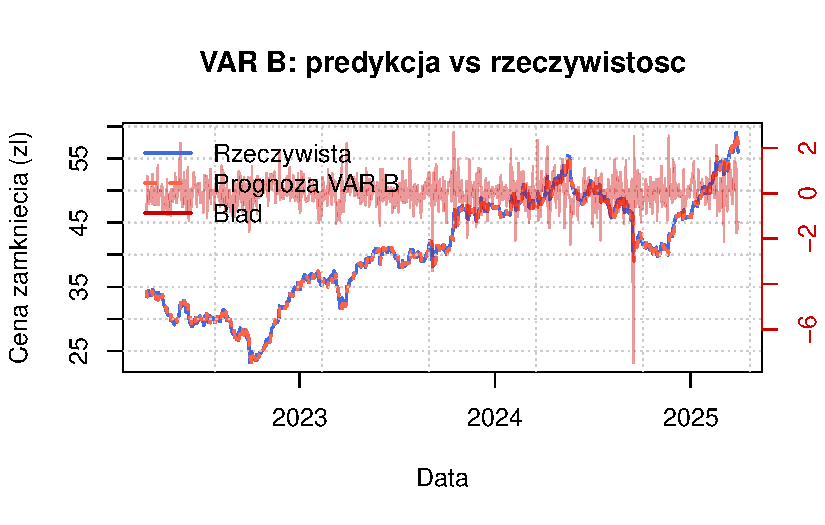
\includegraphics[keepaspectratio]{projekt2_analiza_files/figure-pdf/unnamed-chunk-39-1.pdf}}

}

\caption{VAR B: predykcja vs rzeczywistość (zbiór testowy)}

\end{figure}%

\textbf{Wynik:} dołożenie danych makroekonomicznych \textbf{nie
poprawia} prognozy, a VAR B wypada nawet gorzej niż modelu naiwnego.

{\def\LTcaptype{none} % do not increment counter
\begin{longtable}[]{@{}llll@{}}
\toprule\noalign{}
Model & MAE (zł) & RMSE (zł) & MAPE \\
\midrule\noalign{}
\endhead
\bottomrule\noalign{}
\endlastfoot
Naiwny & 0.522 & 0.740 & 1.31\% \\
VAR A: giełda & 0.523 & 0.740 & 1.31\% \\
VAR B: giełda + makro & 0.528 & 0.745 & 1.33\% \\
\end{longtable}
}

\section{Wyniki}\label{wyniki}

Powód jest spójny z wcześniejszą diagnozą: dane makro zmieniają się
wolno (kwartalnie/miesięcznie) i po synchronizacji schodkowej są w
obrębie okresu stałe, nie niosą więc informacji o \emph{dziennych}
ruchach kursu. Dołożenie trzech zmiennych i dodatkowych parametrów (przy
\(p=10\)) lekko pogarsza wynik pozapróbkowy (delikatne przeuczenie).
Wniosek: na częstotliwości dziennej makro nie pomaga przewidywać kursu
PZU, różnice między modelami mieszczą się w granicach szumu, a
najprostszy model naiwny pozostaje twardym benchmarkiem. Po informację
makro o wyższej wartości predykcyjnej należałoby sięgnąć po model jawnie
mieszanej częstotliwości (np. MIDAS) zamiast wtłaczać
miesięczne/kwartalne dane do dziennego VAR-a.

\section{Wnioski i podsumowanie}\label{wnioski-i-podsumowanie}

\section*{Bibliografia}\label{bibliografia}
\addcontentsline{toc}{section}{Bibliografia}

\protect\phantomsection\label{refs}
\begin{CSLReferences}{1}{0}
\bibitem[\citeproctext]{ref-gus_wskazniki_2026}
Główny Urząd Statystyczny. (2026). \emph{Wskaźniki makroekonomiczne}.
Bazy GUS.
\url{https://bazydanych.new.stat.gov.pl/wskazniki-makroekonomiczne}

\end{CSLReferences}

\renewcommand{\listfigurename}{Spis rysunków}
\listoffigures




\end{document}
